\documentclass[a4paper,12pt]{article}

% comment this if don't want to show answer
\def\withanswer{1}

% For Chinese fonts
% \usepackage{fontspec}
% \setmainfont{SimSun}
\usepackage[AutoFakeBold,SlantFont]{xeCJK}
% \usepackage[SlantFont]{xeCJK}   %AutoFakeBold=true makes CJK characters in the generated PDF can't be copied

\setCJKmainfont{SimSun}

\usepackage[usenames,dvipsnames]{pstricks}
\usepackage{pstricks-add}  % For \psrotate, \psbrace
\usepackage{epsfig}
\usepackage{pst-grad} % For gradients
\usepackage{pst-plot} % For axes
\usepackage{pst-node} % For nodes
\usepackage[space]{grffile} % For spaces in paths
\usepackage{etoolbox} % For spaces in paths

\usepackage{pst-eucl}

\usepackage[english]{babel}     % For enquote
\usepackage{csquotes} 

\usepackage{colortbl}

\usepackage{tikz,fp}
% \usetikzlibrary{angles}         % for perpendicular symbols
\usetikzlibrary{calc,intersections,patterns,angles,quotes}           % 

\usepackage{tkz-euclide} % for perpendicular symbols, \tkzMarkRightAngle, \tkzDefPoint
\usetkzobj{all}

\makeatletter
\def\calcLength(#1,#2)#3{%
  \pgfpointdiff{\pgfpointanchor{#1}{center}}%
               {\pgfpointanchor{#2}{center}}%
  \pgf@xa=\pgf@x%
  \pgf@ya=\pgf@y%
  \FPeval\@temp@a{\pgfmath@tonumber{\pgf@xa}}%
  \FPeval\@temp@b{\pgfmath@tonumber{\pgf@ya}}%
  \FPeval\@temp@sum{(\@temp@a*\@temp@a+\@temp@b*\@temp@b)}%
  \FProot{\FPMathLen}{\@temp@sum}{2}%
  \FPround\FPMathLen\FPMathLen5\relax
  \global\expandafter\edef\csname #3\endcsname{\FPMathLen}
}

\def\drawArc(#1,#2,#3){%
  \pgfmathanglebetweenpoints{\pgfpointanchor{#1}{center}}{\pgfpointanchor{#2}{center}}
  \let\StartAngle\pgfmathresult
  \pgfmathanglebetweenpoints{\pgfpointanchor{#1}{center}}{\pgfpointanchor{#3}{center}}
  \let\EndAngle\pgfmathresult
  \calcLength(#1,#2){myr@dius}
  \draw (#2) arc[start angle=\StartAngle, end angle=\EndAngle, radius=\myr@dius pt];
}
\makeatother

\usepackage{pgfplots}
\pgfplotsset{compat=1.8}

\makeatletter % For spaces in paths
    \patchcmd\Gread@eps{\@inputcheck#1 }{\@inputcheck"#1"\relax}{}{}

    % Font of theorem subtitle
    \def\th@plain{%
      \thm@notefont{}% same as heading font
      \kai % body font
    }
    \def\th@definition{%
      \thm@notefont{}% same as heading font
      \bfseries \kai % body font
    }
\makeatother

\def\answer#1{
  \ifx\withanswer\undefined\else 提示:\par\nopagebreak #1\fi
}

\usepackage{mathtools,amsthm,amsfonts,amssymb,bm}
\usepackage{extarrows}          % for xlongequal
\setCJKfamilyfont{kai}{KaiTi}
\newcommand{\kai}{\CJKfamily{kai}}

% % patch \newtheoremstyle to accept \newline<other tokens>
% \makeatletter
% \patchcmd{\newtheoremstyle}
%  {\def\@tempb{\newline}}
%  {\def\@tempb{\newline}\edef\@tempa{\unexpanded\expandafter{\@car#8\@nil}}}
%  {}{}
% \patchcmd{\newtheoremstyle}
%  {\def\thmheadnl{\newline}}
%  {\def\thmheadnl{#8}}
%  {}{}
% \makeatother

\newtheoremstyle{break}% name
  {15pt}%      Space above, empty = `usual value'
  {}%          Space below
  {\kai}%     Body font
  {}%         Indent amount (empty = no indent, \parindent = para indent)
  {\bfseries}% Thm head font
  {.}%        Punctuation after thm head
  %{\newline\hspace*{\parindent}}% Space after thm head: \newline = linebreak
  {5pt plus 1pt minus 1pt}% Space after thm head: \newline = linebreak
  {}%         Thm head spec
\theoremstyle{break}
\newtheorem{theorem}{\kai 定理}[section]
\newtheorem{example}[theorem]{\kai 例} % Use the same counter as theorem
\newtheorem{property}[theorem]{\kai 性质} % Use the same counter as theorem
\newtheorem{question}[theorem]{\kai 题} % Use the same counter as theorem
\newtheorem{definition}[theorem]{\kai 定义} % Use the same counter as theorem
\newtheorem{corollary}{\kai 推论}[theorem]  % Reset after every theorem
\newtheorem{lemma}[theorem]{\kai 引理}  % Use the same counter as theorem
% \renewcommand*{\proofname}{证明}
\newcommand{\note}{\begingroup\bfseries\kai 注:\endgroup}
\newcommand{\think}{\begingroup\bfseries\kai 思考:\endgroup}
\newcommand{\hints}{\begingroup\bfseries\kai 提示:\endgroup}

\newcommand{\kurschak}{K\"ursch\'ak}
\newcommand{\term}[1]{\begingroup\bfseries\kai{#1}\endgroup}

\DeclareMathOperator{\atan}{atan}

% w/o using the babel package
% \renewcommand{\figurename}{\kai 图}
% w/ babel packge and English as language
\addto\captionsenglish{\renewcommand{\figurename}{\kai 图}}

% Change colon(:) in figure caption to period(.)
\usepackage{caption}
\captionsetup{labelsep=period}

\newcommand{\norm}[1]{\left\lVert{#1}\right\rVert}
\renewcommand*{\vec}[1]{\mathbf{#1}}
\renewcommand*{\le}{\leqslant}
\renewcommand*{\ge}{\geqslant}
\renewcommand*\labelenumi{(\theenumi)}

% Make proof environemtn skip the first line
\makeatletter
\renewenvironment{proof}[1][证明]{\par
  \pushQED{\qed}%
  \normalfont \topsep6\p@\@plus6\p@\relax
  \trivlist
  \item[\hskip\labelsep
    \bfseries \kai%\itshape
    #1\@addpunct{.}]%\mbox{}\\*% new line after \proofname
}{%
  \popQED\endtrivlist\@endpefalse
}
\makeatother

% \newcommand*{\max}[1]{\begingroup\mathrm{max}\left(#1\right)\endgroup}
% \newcommand*{\min}[1]{\mathrm{min}\left(#1\right)}

\renewcommand{\baselinestretch}{1.1}
\renewcommand*{\arraystretch}{1.5}

\usepackage{graphicx}%\resizebox
\graphicspath{{images/}} %Setting the graphicspath

\usepackage[makeroom]{cancel} % for xcancel/cancel/bcancel etc.

\usepackage{fancyvrb}           % for BVerbatim environment

\usepackage{verbatim}
\usepackage{varwidth}
% Center verbatim environment, with the help from verbatim package
\makeatletter
\def\verbatim@font{\normalfont\ttfamily\kai\Large
  \hyphenchar\font\m@ne
  \@noligs}
\makeatother
\newenvironment{pcontent}{%
  \par
  \centering
  \varwidth{\linewidth}%
  \verbatim
}{%
  \endverbatim
  \endvarwidth
  \par\vskip10pt
}

\newcommand{\ptitle}[1]{\par\vskip20pt{\centering\bfseries\kai\Large{#1}\par}\nopagebreak\vskip5pt\nopagebreak}
\newcommand{\pauthor}[1]{\par{\centering\kai【{#1}】\par}\nopagebreak\vskip10pt}
\newcommand{\premark}[1]{\par\kai\small【注释】{#1}\par\vskip5pt}
\newcommand{\ppreface}[1]{{\setlength{\parindent}{2em}\small\kai{#1}}\par\vskip5pt}

% \par indent
\usepackage{indentfirst}
% parindent to 2 characters
\setlength{\parindent}{2em}
\setlength{\parskip}{3pt}

\usepackage{ifthen}             % for \ifelsethen, \whiledo
% \ifthenelse{CONDITION}{POSITIVE}{NEGATIVE}
%     2 is an \ifthenelse{\isodd{2}}{ODD}{EVEN} number.
% \whiledo{CONDITION}{LOOP CONSTRUCT}
%     \newcounter{X}
%     \whiledo{\value{X}<10}{\value{X},\stepcounter{X}}

% 3 counters for loops
\newcounter{X}
\newcounter{Y}
\newcounter{Z}

\include{myconfig}

% comment this when compile the whole document
% \includeonly{proofs-without-words}
% \includeonly{golden-ratio}

\begin{document}



\section{数论}
\label{sec:number-theory}

\begin{example}
  将正整数分成若干子集,使得任意正整数$x$与$2x$不在同一个子集内。则最少只需要两个子集。
\end{example}
\begin{proof}
  按大小顺序依次安放各数,奇数可以随便放,因其不是任意整数的两倍。放偶数$n$时,只要放入$n/2$所在的另一个子集即可。

  另一种方法,任意正整数可以唯一地写为$2^km$的形式,其中$m$是正奇数,$k$是非负整数。若$n_1=2^{k_1}m_1 = 2n_2=2\cdot 2^{k_2}m_2$,则$k_1=k_2+1$其奇偶性不同。将正整数按上述分解中$k$的奇偶性分成两类,每类作一个子集即可。
\end{proof}

\section{黄金比例}
\label{sec:golden-ratio}

\begin{definition}
  将线段分为长短两截,若短的一截比长的一截等于长的一截比原线段的长度,则此分割为\term{黄金分割}。
\end{definition}

记原线段长度为L,在黄金分割下,长一截长度为$l$,短的一截长度为$s$,则
\begin{align*}
  &\frac sl=\frac lL,\quad l+s=L\\
  \implies& \frac sl=\frac l{l+s}
\end{align*}
从而有
\begin{align*}
  \frac ls=\frac{\sqrt5+1}2\approx 1.618, \quad \frac sl=\frac{\sqrt5-1}2\approx 0.618
\end{align*}
以上两个常数都称为\term{黄金比例},通常用$\phi$和$\Phi$表示,即
\begin{align*}
  \phi\equiv\frac{\sqrt5+1}2,\quad \Phi\equiv\frac{\sqrt5-1}2
\end{align*}

\begin{question}
  证明下列恒等式:
  \begin{align*}
    \phi\cdot\Phi=1,\quad \phi=\Phi+1,\quad \phi^2=\phi+1,\quad \frac1\phi=\phi-1
  \end{align*}
\end{question}

\begin{example}[连分数表示]\label{ex:phi-of-continued-fraction}
  \begin{align}
    \phi = 1 + \dfrac1{1 + \dfrac1{1+\dfrac1{1+\dfrac1{1+\cdots}}}}
  \end{align}
\end{example}
\begin{proof}
  利用$\phi=1+\dfrac1\phi$,设连分数为$x$,则
  \begin{align*}
    \frac1{x-1}=x\implies x^2-x-1=0\implies x=\frac{1\pm\sqrt5}2
  \end{align*}
  由$x>0$可知$x=\dfrac{1+\sqrt5}2=\phi$。
\end{proof}

\begin{definition}
  以下数值称为\term{贵金属分割}:
  \begin{align}
    \frac{n+\sqrt{n^2+4}}2,\quad\quad n=1,2,3,\cdots
  \end{align}
  当$n=1$时为黄金分割$\dfrac{\sqrt5+1}2$;当$n=2$时为\term{白银分割}$\sqrt2+1$;当$n=3$时为\term{青铜分割}$\dfrac{\sqrt{13}+3}2$。
\end{definition}
\begin{question}
  证明:贵金属分割都可以用以下的连分数形式表示
  \begin{align*}
    \frac{n+\sqrt{n^2+4}}2=
    n+\dfrac1{n+\dfrac1{n+\dfrac1{n+\dfrac1{n+\dfrac1{n+\cdots}}}}}
  \end{align*}
\end{question}

\begin{example}[平方根表示]
  \begin{align}
    \phi=\sqrt{1+\sqrt{1+\sqrt{1+\sqrt{1+\sqrt{1+\cdots}}}}}
  \end{align}
\end{example}
\begin{proof}
  记等号右边为$x$,则$x^2 = 1 + x$,余下与题~\ref{ex:phi-of-continued-fraction}相同,略。
\end{proof}

\begin{example}[三角函数表示]
  $\phi=1 + 2\sin18^\circ.$
\end{example}
\begin{proof}
  由$\phi=1+\Phi$,等价于证明$\sin18^\circ=\dfrac\Phi2$。令$x\equiv18^\circ$,则$2x+3x=5x=90^\circ$,应用以下公式
  \begin{align*}
    \sin 2x &= \cos \left(\frac\pi2 - 2x\right) = \cos 3x\\
    \sin 2x &=2\sin x\cos x\\
    \cos 3x &= 4\cos^3x-3\cos x
  \end{align*}
  可得
  \begin{align*}
    &2\sin x\cos x = 4\cos^3x-3\cos x\\
    \implies& \cos x(2\sin x - 4\cos^2 x + 3) = 0  & (cos x\ne 0)\\
    %\overset{\cos x\ne 0}{\implies} & 2\sin x + 4\sin^2 x - 1 = 0
    \implies & 2\sin x + 4\sin^2 x - 1 = 0 
  \end{align*}
  从而有
  \begin{align*}
    \sin x = \dfrac{-2\pm\sqrt{20}}{8}=\dfrac{-1\pm\sqrt5}4
  \end{align*}
又$x=18^\circ$,显然$\sin x>0$,从而有
\begin{align*}
  \sin18^\circ&=\sin x =\dfrac{\sqrt5-1}4=\dfrac\Phi2\qedhere
\end{align*}
\end{proof}

\begin{example}[黄金长方形]
  长宽比满足黄金比例的长方形称为\term{黄金长方形},如下图。\par
  \begin{center}
    \begin{tikzpicture}[scale=2.5];
      \draw(0,0)rectangle($({.5*(sqrt(5)+1)},1)$);
    \end{tikzpicture}
  \end{center}
\end{example}

\begin{example}[尺规作图]
  找出线段$AB$的黄金分割点。
\end{example}
关键点在于作出$\sqrt5$的长度,作出一个边长分别为$1,2,\sqrt5$的直角三角形。这里取$AB$的长度为$2$,则
\begin{enumerate}
\item 找出$AB$的中点$O$,则$AO=BO=1$;
\item 以$AO$为长度在过点$B$的$AB$垂直线上找点$C$,使$BC=AO=1$,则$AC=\sqrt5$;
\item 在$AC$上找点$D$,使$DC=BC=1$,此时$AD=\sqrt5-1$;
\item 在$AB$上找点$S$,使$AS=AD=\sqrt5-1$,从而$\dfrac{AS}{AB}=\dfrac{\sqrt5-1}{2}$,即点$S$是$AB$的黄金分割点。
\end{enumerate}
% \begin{figure}[htbp]
\begin{center}
  % \centering%\fbox{
  \vspace*{-5cm}
  \begin{tikzpicture}[scale=3]
    \coordinate[label=below left:$A$] (A) at (0,0);
    \coordinate[label=below right:$B$] (B) at (2,0);
    \coordinate[label=above:$C$] (C) at (2,1);
    \coordinate (O) at (1,0);
    \tkzInterLC(A,C)(C,B)\tkzGetPoints{D}{};
    \tkzInterLC(A,B)(A,D)\tkzGetPoints{}{S}\tkzLabelPoints[below](O,S)
    \calcLength(A,D){AD}
    %\draw(S) arc(0:40:\AD pt);
    \tkzMarkRightAngle[color=blue](A,B,C)
    \drawArc(A,S,D)
    \draw(A)--(O) node[midway,sloped]{||} -- (B)--(C) node[midway,sloped]{||}--(D)node[midway,sloped]{||} --cycle;
    % \draw(B) arc(270:200:1);
    \drawArc(C,B,D);
    \tkzDrawPoints(A,B,C,O,D,S);

    \clip(-1,0)rectangle(3,1);
  \end{tikzpicture}
%}
\end{center}
%   \caption{黄金分割的尺规作图}
%   \label{fig:golden-ratio-of-ruler-and-compass-construction}
% \end{figure}

\begin{definition}
  腰与底边的长度比是$\phi$的等腰三角形称为\term{黄金三角形}。
\end{definition}
\note 有时把腰与底边的长度比是$\Phi$的等腰三角形也称为黄金三角形。但此处只考虑比值是$\phi$的情况,即腰比底长的等腰三角形。


\begin{definition}
  等腰三角形的一条底角平分线将三角形分为两个三角形,若含底边的小三角形与原三角形相似,则称原三角形为\term{黄金三角形}。
\begin{center}
    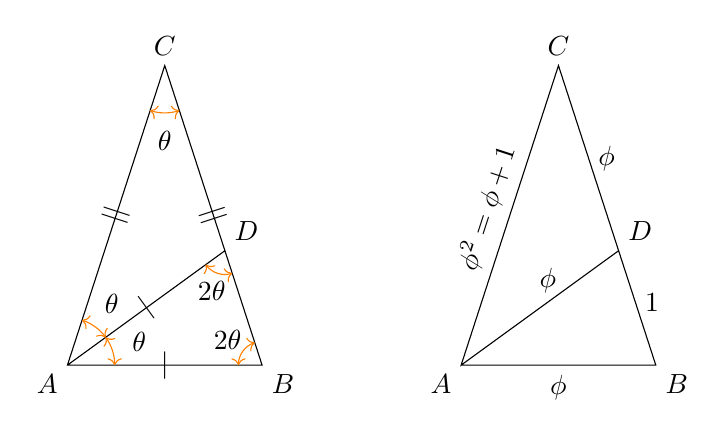
\begin{tikzpicture}[scale=1];
      \begin{scope}[shift={(0,0)}]
        \coordinate(A) at (0,0);
        \coordinate(C) at (72:4);
        \coordinate(B) at ($(C)!1!36:(A)$); %rotate A to 36 degree around C
        \tkzDefLine[bisector](C,A,B)\tkzGetPoint{D'}
        \tkzInterLL(A,D')(B,C)\tkzGetPoint{D}
        \draw(A)--(B)node[midway,sloped]{|}--(C)node[midway,sloped]{||}--cycle node[midway,sloped]{||}--(D)node[midway,sloped]{|};
        \draw pic["$\theta$",<->,draw=orange,angle eccentricity=1.6,angle radius=.6cm]{angle=D--A--C};
        \draw pic["$\theta$",<->,draw=orange,angle eccentricity=1.6,angle radius=.6cm]{angle=B--A--D};
        \draw pic["$\theta$",<->,draw=orange,angle eccentricity=1.6,angle radius=.6cm]{angle=A--C--B};
        \draw pic["$2\theta$",<->,draw=orange,angle eccentricity=1.8,angle radius=.3cm]{angle=C--B--A};
        \draw pic["$2\theta$",<->,draw=orange,angle eccentricity=1.8,angle radius=.3cm]{angle=A--D--B};
        \tkzLabelPoints[below left](A)
        \tkzLabelPoints[below right](B)
        \tkzLabelPoints[above](C)
        \tkzLabelPoints[above right](D)
      \end{scope}
      \begin{scope}[shift={(5,0)}]
        \coordinate(A) at (0,0);
        \coordinate(C) at (72:4);
        \coordinate(B) at ($(C)!1!36:(A)$); %rotate A to 36 degree around C
        \tkzDefLine[bisector](C,A,B)\tkzGetPoint{D'}
        \tkzInterLL(A,D')(B,C)\tkzGetPoint{D}
        \draw(A)--(B)node[midway,sloped,below]{$\phi$}
                --(D)node[pos=.55,right]{$1$}
                --(C)node[midway,right]{$\phi$}
                --(A)node[midway,sloped,above]{$\phi^2=\phi+1$}
                --(D)node[pos=.55,above]{$\phi$};
        \tkzLabelPoints[below left](A)
        \tkzLabelPoints[below right](B)
        \tkzLabelPoints[above](C)
        \tkzLabelPoints[above right](D)
      \end{scope}
    \end{tikzpicture}
  \end{center}
\end{definition}

\begin{theorem}
  一个等腰三角形是黄金三角形的充要条件是其顶角是$\dfrac\pi5(36^\circ)$。
\end{theorem}
\begin{proof}
  必要性:由图,$5\theta=\pi$,从而$\theta=\dfrac\pi5$。

  充分性:若等腰三角形顶角$\angle C=\dfrac\pi5$,则容易计算到到$\angle BAD=\dfrac\pi5$,从而$\triangle ABC\sim\triangle BAD$,即$\triangle ABC$是黄金三角形。
\end{proof}

\begin{question}
  证明黄金三角形各边长度的比例关系如上图所示。
\end{question}

\begin{question}
  证明正五角星(Regular Pentagram)的顶点可组成黄金三角形。
  \begin{center}
    
\begin{tikzpicture}[scale=.6]
      \coordinate(A) at ( 18:4);
      \coordinate(B) at ( 90:4);
      \coordinate(C) at (162:4);
      \coordinate(D) at (234:4);
      \coordinate(E) at (306:4);
      \draw(A)--(C)--(E)--(B)--(D)--cycle;
    \end{tikzpicture}
  \end{center}
\end{question}

\begin{example}[数值逼近]
  $\phi$是方程$x^2-x-1=0$的一个解,应用牛顿迭代法(Newton's method)逐渐逼近$\phi$。
\end{example}

选择初始点$x_0=3$,利用牛顿迭代公式
\begin{align*}
  x_{n+1}=x_n-\frac{f(x_n)}{f'(x_n)}=x_n-\frac{x_n^2-x_n-1}{2x^n-1}=\frac{x_n^2+1}{2x^n-1}
\end{align*}
从而有
\begin{align*}
  x_0&=3 &
  x_1&=2\\
  x_2&=1.66666666666667 &
  x_3&=1.61904761904762\\
  x_4&=1.61803444782168 &
  x_5&=1.61803398874999\\
  x_6&=1.61803398874989 &
  x_7&=1.61803398874989
\end{align*}
可以看出已经开始向$\phi$收敛,在上述保留14位小数的精度下迭代到$x_7$已经不变了。牛顿迭代法特别适合于应用计算机对方程进行数值求解。

\section{函数}
\label{sec:function}

\begin{definition}[对合,Involution]
  一个函数若存在反函数且其反函数为其本身,则称此函数为对合或对合函数。
\end{definition}

\begin{example}
  以下三个都是对合函数的例子:
  \begin{align*}
    f(x)=x,\quad g(x)=\frac1x,\quad h(x)=\frac{x}{x-1}
  \end{align*}
\end{example}

\begin{example}
  存在无限个对合函数。
\end{example}
\begin{proof}
  显然,一个函数是对合函数$\iff$其在笛卡尔坐标下的曲线关于直线$y=x$对称,这样的曲线是可以无限地构造出来。比如任意非零实数$a$,$f(x)=\frac{a}{x}$都是对合函数。或者,利用下面的定理构造。
\end{proof}

\begin{theorem}
  若$f$是对合函数,$g$有反函数$\bar g$,则$h\equiv g\circ f\circ\bar g$是对合函数。
\end{theorem}
\begin{proof}
  任意定义域内$x$,有
  \begin{align*}
    h(x)&= g(f(\bar g(x)))\\
    h(h(x))&=g(f(\underline{\bar g( g}(f(\bar g(x))) ))) = g(\underline{f(f}(\bar g(x)))) = g(\bar g(x)) = x \qedhere
  \end{align*}
\end{proof}


\section{单调函数}
\label{sec:monotonic-functions}

\begin{example}
  任意非负数$a,b,c$满足$a\le b+c$,则
  \begin{align*}
    \frac{a}{1+a}\le \frac{b}{1+b} + \frac{c}{1+c}
  \end{align*}
  并说明等号成立的充要条件。
\end{example}

\begin{proof}
  容易知道$f(x)=\dfrac{x}{1+x}$在$x\ge0$时是严格单调递增函数,从而
  \begin{align*}
    \frac{a}{1+a}&\le\frac{b+c}{1+b+c}&\text{等号成立}\iff a=b+c\\
    &=\frac{b}{1+b+c} + \frac{c}{1+b+c}\\
    &\le\frac{b}{1+b} + \frac{c}{1+c}&\text{等号成立}\iff b=c=0
  \end{align*}
  从而原不等式得证,且当且仅当$a=b=c=0$时等号成立。
\end{proof}

\chapter{度量空间}
\label{chap:metric-space}

容易知道,对$\forall x,y,z$,欧氏空间中的距离满足以下性质:
\begin{enumerate}
\item 非负性。即$d(x,y)\ge0.$
\item {\color{red}同一性?}。即$d(x,y)=0\iff x=y.$
\item 对称性。即$d(x,y)=d(y,x).$
\item 三角不等式。即$d(x,y)\le d(x,z)+d(z,y).$
\end{enumerate}

上面的非负性可以由其余三条性质推出(请自行推导)。任意空间中二元函数若满足上述的{\color{red}同一性?}、对称性及三角不等式,则称其为欧氏空间中的一个度量,也称为距离。点集配上度量,就是一个度量空间。

\begin{definition}[度量空间,Metric Space]
  点集$\mathcal{S}$,$d$是$\mathcal{S}$上的一个度量,则称$(\mathcal{S},d)$为一个度量空间。
\end{definition}

\begin{definition}[柯西序列,Cauchy Sequence]
  序列$x_1,x_2,x_3,\cdots$,若对任意正数$\epsilon$,存在正整数$N_\epsilon$,使得$\forall m,n>N_\epsilon$,有$d(x_m,x_n)<\epsilon$,则称此序列是度量$d$下的柯西序列。
\end{definition}

柯西序列是越到后面越密集的序列。若柯西序列在$\mathcal{S}$收敛,则其收敛点是唯一的(请自行推导。\hints 反证)。

\begin{definition}[完备性]
  若一个度量空间中的任意柯西序列都收敛于空间中某一个点,则称此度量空间是完备的。
\end{definition}

\begin{example}[有理数集]
  证明有理数集在普通实数距离下不是完备的。
\end{example}
\begin{proof}[解释]
  在实数轴上,有理数集是有“洞”的,而填充这些洞的就是无理数。用有理数构造一个柯西序列,使其收敛于某个无理数,即可得证。比如可以利用$\phi$的连分数表示来构造,即
  \begin{align*}
    x_1=1,\quad x2=1+\frac1{x_1},\quad x_3=1+\frac1{x_2},\cdots &\qedhere
  \end{align*}
\end{proof}


\chapter{不动点}
\label{chap:fixed-point}

本节内容需要拓扑与泛函分析的知识,不需深究。

\begin{example}
  两张内容一样的地图,把小地图放在大地图上,使小地图完全在大地图内,则必有一点,使两张地图上对应的点代表同一个物理位置。
\end{example}

此问题也有另外一种描述方式:把一张地图放在地上,则地图上必有一点正好在它所代表的物理位置的正上方。在这种描述里,大地图对应于所在城市/国家/甚至地球,小地图则对应于地上的地图。

要回答这问题,需要用到\term{不动点}理论。点$x$称为是映射$f$的不动点,若$f(x)=x$,即对不动点映射过后的像不动,还是落在自身。不动点定理表明在某些条件下,映射至少有一个不动点。

\begin{definition}[压缩映射]
  距离空间$\mathcal{D}$上的映射$f:\mathcal{D}\to\mathcal{D}$称为是压缩映射,若存在$q\in[0,1)$,使得任意$x,y$有
  \begin{align}
    d(f(x),f(y))\le q d(x,y)
  \end{align}
\end{definition}

\begin{theorem}[巴拿赫不动点定理,压缩不动点定理,Banach fixed-point theorem]
  完备距离空间上压缩映射存在唯一的不动点$x^*$,且由任意一点$x_0$通过以下迭代:
  \begin{align*}
    x_{n}=f(x_{n-1}),\quad\quad n=1,2,3,\cdots
  \end{align*}
  有$x_n\to x^*$。
\end{theorem}
\begin{proof}
  需要用到拓扑与泛函分析的知识,此处略过。
\end{proof}

回到大小地图的问题,在大小地图所在平面上建立坐标系,考虑将大地图上的点对应的坐标$x$映射到小地图上的点对应的坐标$x'$的映射$f$,其中$x$与$x'$在大小地图上表示同一个物理位置,则容易知道$f$是一个压缩映射,因为每两个点的距离都被压缩了。从而由巴拿赫定理,存在唯一的不动点。

\chapter{恒等式}
\label{chap:identities}

\section{基本恒等式}
\label{sec:basic-identities}

\begin{example}[两数和的幂]$\forall a,b\in\mathcal{R}$,有
  \begin{align*}
    (a + b)^2 &= a^2 + 2ab + b^2\\
    (a + b)^3 &= a^3 + 3a^2b + 3ab^2 + b^3\\
    (a + b)^4 &= a^4 + 4a^3b + 6a^2b^2 + 4ab^3 + b^4
  \end{align*}
\end{example}
对于$(a-b)^2$及$(a-b)^3$这种,只要在上式中把$b$换为$-b$即可。观察上述$(a+b)^n$的系数,可以发现其与下面的杨辉三角是一致的:
\begin{center}
  \begin{tikzpicture}[scale=1.0]
    \begin{scope}[shift={(.5,1)}]
      \foreach \x/\v in {1/1,2/1}{%
        \node at (\x,0) {\v};
      }
    \end{scope}
    \begin{scope}[shift={(0,0)}]
      \foreach \x/\v in {1/1,2/2,3/1}{%
        \node at (\x,0) {\v};
      }
    \end{scope}
    \begin{scope}[shift={(-.5,-1)}]
      \foreach \x/\v in {1/1,2/3,3/3,4/1}{%
        \node at (\x,0) {\v};
      }
    \end{scope}
    \begin{scope}[shift={(-1,-2)}]
      \foreach \x/\v in {1/1,2/4,3/6,4/4,5/1}{%
        \node at (\x,0) {\v};
      }
    \end{scope}
    \begin{scope}[shift={(-1.5,-3)}]
      \foreach \x/\v in {1/1,2/5,3/10,4/10,5/5,6/1}{%
        \node at (\x,0) {\v};
      }
    \end{scope}
    \foreach \y in{1,2,3,4,5}{%
      \node[left] at (-2,2-\y){$n=\y$};
    }
  \end{tikzpicture}
\end{center}


\begin{example}[配方]$\forall a\ne 0$,有
  \begin{align*}
    ax^2 + bx + c = a\left(x-\frac{b}{2a}\right)^2 + \frac{4ac - b^2}{4a}
  \end{align*}
\end{example}

\section{代数}
\label{sec:algebra-identities}

\begin{theorem}[Sophie-Germain恒等式]
  $\forall x,y$,有
  \begin{align*}
    x^4 + 4y^4 = (x^2 + 2xy + 2y^2)(x^2 - 2xy + 2y^2)
  \end{align*}
\end{theorem}
在上式中令$x=1$,可以得到哥德巴赫定理;令$y=1$,则可以得到吉梅茵定理。
\begin{theorem}[哥德巴赫定理,Goldbach Theorem]\mbox{}\par
  对任意整数$n>1$,$4n^4+1=(1+2n+2n^2)(1-2n+2n^2)$是合数。  
\end{theorem}
\begin{theorem}[吉梅茵定理,Germain Theorem]\mbox{}\par
  任意整数$n>1$,$n^4+4=(n^2+2n+2)(n^2-2n+2)$是合数。
\end{theorem}


\begin{theorem}[贝祖定理,B\'ezout's identity]\label{th:Bezout}
  $\forall a,b\in\mathcal{Z},\exists x,y\in\mathcal{Z}$使得
  \begin{align*}
    ax+by=\mathrm{gcd}(a,b)
  \end{align*}
  若$a,b$互质,则有$ax+by=1$。
\end{theorem}

\begin{theorem}\label{th:inverse-bezout}
  若整数$x,y,a,b$满足$ax+by=1$,则$x,y$互质。从而$\gcd(a,b)=\gcd(a,y)=\gcd(x,b)=\gcd(x,y)=1$。
\end{theorem}
\begin{proof}
  记$g=\gcd(x,y)$,则$x'=x/g$与$y'=y/g$是互质的两个整数,代入有
  \begin{align*}
    1=ax+by=ax'g+by'g=g(ax'+by')
  \end{align*}
  从而$g\mid 1\implies g=1$。
\end{proof}

%%% $x,y$称为$(a,b)$的B\'ezout系数。一般来说,$(a,b)$的B\'ezout系数$x,y$不是唯一的,可以通过扩展欧几里得算法来计算得到。
$x,y$称为$(a,b)$的B\'ezout系数。一般来说,$(a,b)$的B\'ezout系数$x,y$不是唯一的,可以通过类似于欧几里得辗转相除法得到。

\begin{example}
  求整数$a,b$使得$211a+37b=1$。
\end{example}
\begin{proof}[提示]
\begin{align*}
  211a+37b=1 &\iff 37b=1-211a \\
             &\iff b=\frac{1-211a}{37}=-5a+\frac{1-26a}{37}\\
             &\iff b=-6a+\frac{1+11a}{37} 
\end{align*}
令$1+11a=37t_1$,其中$t_1$为整数,从而
\begin{align*}
  1+11a=37t_1 & \iff a=\frac{37t_1-1}{11}=3t_1 + \frac{4t_1-1}{11}
\end{align*}
令$4t_1-1=11t_2$,其中$t_2$为整数,则$t_1=2t_2+(3t_2+1)/4$。若能观察出来取$t_2=1$可使$t_1$为整数,则代入即可。

若观察不出来,继续令$3t_2+1=4t_3$,则$t_2=t_3+(t_3-1)/3$,若还观察不出来$t_3$应取什么值可使$t_2$为整数,继续令$t_3-1=3t_4$,从而$t_3=3t_4+1$,整数$t_4$可随意挑选,再一步步反向代入,可得$t_3,t_2,t_1,a,b$。
\end{proof}


% \begin{definition}[扩展欧几里得算法]
%   Ref. \verb|https://en.wikipedia.org/wiki/Extended_Euclidean_algorithm|
% \end{definition}

\begin{example}[1959 IMO]
  求证对任意正整数$n$,分数$\dfrac{21n+4}{14n+3}$不可约。
\end{example}
\begin{proof}[提示]
  相当于证明$21n+4$与$14n+3$互质。尝试使用定理\ref{th:inverse-bezout},若能找到两个整数$a,b$,使得$a(21n+4)+b(14n+3)=1$,则有$21n+4$与$14n+3$互质。而
  \begin{align*}
    a(21n+4)+b(14n+3)=1 \iff (21a + 14b)n + 4a + 3b = 1
  \end{align*}
  而上式要对任意整数$n$成立,等价于以下两式同时成立
  \begin{align*}
    21a+14b=0, \quad 4a+3b=1
  \end{align*}
  而这个方程组是有整数解$a=-2, b=3$,从而原问题得证。
\end{proof}

\begin{example}\label{ex:sum-is-negative-to-product}
  对任意满足$a+b\ne0$,$b+c\ne0$,$c+a\ne0$的实数$a,b,c$,则以下三个数的和与积互为相反数:
  \begin{align*}
    \frac{a-b}{a+b},\quad \frac{b-c}{b+c},\quad \frac{c-a}{c+a}
  \end{align*}
  即
  \begin{align*}
    \frac{a-b}{a+b} + \frac{b-c}{b+c} + \frac{c-a}{c+a} 
    + \frac{a-b}{a+b} \cdot \frac{b-c}{b+c} \cdot \frac{c-a}{c+a} = 0
  \end{align*}
\end{example}
\begin{proof}
  引入几个记号:
  \begin{align*}
    S_{l}\equiv&\, \frac{a-b}{a+b} + \frac{b-c}{b+c} + \frac{c-a}{c+a} \\
    S_{r}\equiv&\,\frac{a-b}{a+b} \cdot \frac{b-c}{b+c} \cdot \frac{c-a}{c+a}\\
    P\equiv&\,S_{r}\cdot (a+b)(b+c)(c+a) = (a-b)(b-c)(c-a)
  \end{align*}
  则问题中的等式等价于
  \begin{align*}
    S_{l}\cdot (a+b)(b+c)(c+a) + P = 0
  \end{align*}
  最直接的方法,是逐项展开,合并同类项。
  \begin{align*}
     &\, S_{l}\cdot (a+b)(b+c)(c+a)\\
    =&\, (a-b)(b+c)(c+a) + (b-c)(c+a)(a+b) + (c-a)(a+b)(b+c)\\
    =&\, (c+a)\left( (a-b)(b+c) + (b-c)(a+b) \right) + (c-a)(a+b)(b+c)\\
    =&\, 2b(c+a)(a-c) + (c-a)(a+b)(b+c)\\
    =&\, (a-c)(2bc+2ab - (ab+ac+bb+bc))\\
    =&\, (a-c)(bc+ab - ac-bb)\\
    =&\, (a-c)(c(b-a)+b(a-b))\\
    =&\, (a-c)(b-a)(c-b)\\
    =&\, -(a-b)(b-c)(c-a) = -P&&\qedhere
  \end{align*}
\end{proof}

\begin{example}
  若$a=3,b=4,c=5$,则
  \begin{align*}
    \frac{a-b}{a+b} = \frac{3-4}{3+4} = -\frac17\\
    \frac{b-c}{b+c} = \frac{4-5}{4+5} = -\frac19\\
    \frac{c-a}{c+a} = \frac{5-3}{5+3} = \phantom{-}\frac14
  \end{align*}
  其和为
  \begin{align*}
    -\frac17 - \frac19 + \frac14 = \frac{-9\times4 - 7\times4 + 7\times9}{4\times7\times9} = -\frac1{4\times7\times9}
  \end{align*}
  容易看出,其和为其积的相反数。
\end{example}

\section{重要恒等式}
\label{sec:important-identities}

以下几个恒等式不常见,却是竞赛中的常客。虽无需记忆,但可以留点印象,知道有这么回事,对解题有大帮助。

\begin{example}\label{ex:product-of-four-continuous-integer}
  证明对任意$x\in\mathcal{R}$,有
  \begin{align*}
    x(x+1)(x+2)(x+3)+1=\left( x^2+3x+1\right )^2
  \end{align*}
\end{example}
展开两边可得。换一个形式,则有
\begin{align*}
  \sqrt{x(x+1)(x+2)(x+3)+1}= x^2+3x+1 = (x + 1)^2 + x
\end{align*}


\begin{example}
  求$\sqrt{2019\times2020\times2021\times2022+1}-2020^2$。

  在恒等式$\sqrt{x(x+1)(x+2)(x+3)+1}= x^2+3x+1 = (x + 1)^2 + x$中令$x=2019$,则有
  $\sqrt{2019\times2020\times2021\times2022+1}-2020^2=2019$。
\end{example}

\begin{theorem}[Fibonacci Identity]任意实数$a,b,c,d$,有恒等式
  \begin{align*}
    \left(a^2+b^2\right)\left(c^2+d^2\right)
    = \left(ac +  bd\right)^2 + \left(ad -  bc\right)^2
    = \left(ac -  bd\right)^2 + \left(ad +  bc\right)^2 
  \end{align*}
\end{theorem}


\begin{theorem}
  若$\alpha, \beta, \gamma$均非$\pi/2$的奇数倍,则等式
  \begin{align*}
    \tan\alpha +\tan\beta+\tan\gamma=\tan\alpha \cdot \tan\beta \cdot \tan\gamma
  \end{align*}
  当且仅当$\alpha+\beta+\gamma$是$\pi$的整数倍时成立。
\end{theorem}

\section{完全平方数}
\label{sec:perfect-squares}

\begin{example}[1953 \kurschak]
  $\forall n\in\mathcal{Z}^+$,若正整数$d$整除$2n^2$,则$n^2+d$不是完全平方数。
\end{example}

\hints 反证。令$d=2n^2/k$,若$n^2+d=n^2+2n^2/k=m^2$,则$(mk)^2=n^2(k^2+2k)$,从而$k^2+2k$也是一个完全平方数。然而$k^2<k^2+2k<k^2+2k+1=(k+1)^2$,即$k^2+2k$位于两个相邻的完全平方数之间,从而不能是完全平方数,矛盾。

\chapter{抽屉原理}
\label{chap:pigeonhole-principle}

\section{原理}
\label{sec:pigeonhole-principle-theory}

\begin{theorem}[抽屉原理,鸽笼原理,鸽巢原理,Pigeonhole principle]
  若有$n$个笼子和$kn+1$只鸽子,所有的鸽子都被关在鸽笼里,那么至少有一个笼子有至少$k+1$只鸽子。
\end{theorem}

\begin{proof}
  反证法,若每个笼子最多有不超过$k$个鸽子,那么所有笼子鸽子总数不超过$kn$个,与原来有$kn+1$个鸽子矛盾。
\end{proof}

当$k=1$时,是抽屉原理最直观的情况:若有$n$个笼子和$n+1$只鸽子,所有的鸽子都被关在鸽笼里,那么至少有一个笼子有至少$2$只鸽子,即装有不少于两个鸽子的笼子数最少是$1$。

\think 若上面$n+1$只鸽子换成$n+1,n+2,\cdots$是否成立?对于$2n-1$、$2n$及$2n+1$只鸽子,又可以得到什么样的结论?

\begin{example}
  普遍认为成人的头发数量约在10万左右,那么对于深圳的常住人口(按2018年2180万算),基本可以肯定有人有相同的头发数。
\end{example}

\begin{proof}
  按头发数做鸽笼,按统计数据成人头发平均约为10万左右,假设大部分深圳常住人口(比如2180万的80\%>1600万)的头发数量都小于等于1000万根。按抽屉原理可得。
\end{proof}

\begin{example}
  在$1,2,\cdots,100$里任意选51个数,总能在这选出来的数中找到两个互质数。
\end{example}

\begin{proof}
  将100个数按$(1,2), (3,4), \cdots, (99,100)$分为50组,则选51个数总有两个落到同一组中,而同一组的两数互质,从而得证。
\end{proof}

\begin{question}
  在$1,2,\cdots,100$里任意选51个数,总能在这选出来的数中找到两个,使得其中一个被另一个整除。
\end{question}
\hints $\forall a\in\mathcal{Z}^+$,存在奇数$k$及整数$n$,使得$a=k\cdot 2^n$。对所有整数按$k$分类。

\begin{example}
  在任意9个两两不等的实数中,总能选出两个,设其为$a,b$,满足以下条件
  \begin{align*}
    0 < \frac{a-b}{1+ab} < \sqrt2 -1
  \end{align*}
\end{example}

\begin{proof}[提示]
  联想公式
  \begin{align*}
    \tan(\alpha-\beta)=\frac{\tan\alpha-\tan\beta}{1+\tan\alpha\tan\beta}
  \end{align*}

  而$\tan(x)$的周期是$(-\pi/2, \pi/2]$,将区间8等份(让9个数总有两个落入其中一份)为以下8个区间
  \begin{align*}
    (-\frac\pi2, -\frac{3\pi}8], (-\frac{3\pi}8, -\frac\pi4], \cdots, (\frac{3\pi}8, \frac\pi2]
  \end{align*}

  $\forall a, \exists\hat a\in(-\pi/2, \pi/2], s.t. \tan\hat a = a$,从而任意9个实数,总存在两个,记为$a,b$,存在$\hat a, \hat b$落在上述8个区间中的同一个,且有$a=\tan\hat a, b=\tan\hat b$。不妨设$a>b$,从而$0<\hat a-\hat b<\pi/8$,由$\tan(x)$在上述每个区间中均为严格单调递增,有
  \begin{align*}
             & 0 < \tan(\hat a - \hat b) < \tan\frac\pi8\\
    \implies & 0 < \frac{a - b}{1+ab} < \sqrt2 - 1&\qedhere
  \end{align*}
\end{proof}


\begin{question}[XLI Mathematical Olympiad in Poland]
  一个三角形可以放置在一个单位正方形内,且存在一种放置方法使得正方形的中心不在三角形内。那么该三角形有一条边长小于1。
\end{question}

\hints 将正方形划分几份,使得三角形至少有两个顶点落在某份中。

%%%%%%%%%%%%%%%%%%%%
%%% Questions
%%%%%%%%%%%%%%%%%%%%
\begin{question}
  从$1,2,\cdots,100$中任意取11个数字,那么这11个数字组成的集合中,总存在两个不相交的非空子集,其元素之和相等。
\end{question}
\begin{proof}[提示}
11个元素组成的集合,其非空真子集总共有$2^{11}-2=2046$个。
% 其中两两互补,即任意一个总有能找到一个与之互补。从而将11个元素分成两份且每份都至少有一个元素的方法共有$2046\div2=1023$个
而1到100取10个数字(\think 为什么取10个而不是11个?取11个其和已经最大了,没有真子集的和能与其相比了。),其和最大值为$91+92+\cdots+100=955$。从而由抽屉原理,这2045个子集中,总有两个的和是相等的,且显然这两个和相等的子集,没有一个是另一个的真子集(否则其和就不相等了),在这两个子集中去掉相同的元素,就可以得到两个不相交、非空且和相等的集合。
\end{proof}

\begin{question}
  在三维空间中任意选取9个坐标都是整数的点。证明这连接9个点而形成的线段中至少包含另外一个坐标为整数的点
\end{question}

\begin{question}
  任意六个人中,以下两个结论总有一个成立:
  \begin{enumerate}
  \item 其中有三人互相认识。
  \item 其中有三人互相不认识。
  \end{enumerate}
\end{question}

\hints 相当于正六边形的六个顶点用两种颜色的线段两两连接起来,则这些线段组合的三角形中,总存在一个同色的三角形。

\begin{question}
  任意一个16位的正整数的数字所组成的数字串中,总存在一个子串,其数字的乘积是一个完全平方数。
\end{question}

\hints 若16位数中含有数字$0,1,4,9$,那么取这个数字本身组成的子串即可,从而只需考虑由数字$2,3,5,6,7,8$组成的16位数。由于
\begin{align*}
  6 = 2\times 3,\quad 8=2^3
\end{align*}
从而任意一个子串各数字的乘积可以写成如下形式
\begin{align*}
  2^a \times 3^b \times 5^c \times 7^d
\end{align*}
若$a,b,c,d$都是偶数,那么这个子串数字的乘积就是完全平方数。而$a,b,c,d$的奇偶组合数总共有$2^4=16$种,即
\begin{align*}
  \text{(奇奇奇奇)},\quad \text{(奇奇奇偶)},\quad \text{(奇奇偶奇)},\quad \text{(奇奇偶偶)}\\
  \text{(奇偶奇奇)},\quad \text{(奇偶奇偶)},\quad \text{(奇偶偶奇)},\quad \text{(奇偶偶偶)}\\
  \text{(偶奇奇奇)},\quad \text{(偶奇奇偶)},\quad \text{(偶奇偶奇)},\quad \text{(偶奇偶偶)}\\
  \text{(偶偶奇奇)},\quad \text{(偶偶奇偶)},\quad \text{(偶偶偶奇)},\quad \text{(偶偶偶偶)}
\end{align*}

从而至少需要构造17种选取方式。记16位数各数字按顺序分别为$x_1,x_2,\cdots,x_{16}$,令
\begin{align*}
  F(k) =
  \begin{cases}
    1 = 2^0 \times 3^0 \times 5^0 \times 7^0 & k=0\\
    \prod_{i=1}^k x_i = 2^{a_k} \times 3^{b_k} \times 5^{c_k} \times 7^{d_k},&k=1,2,\cdots,16
  \end{cases}
\end{align*}
则$F(0),F(1),\cdots,F(16)$这17个数中至少有两个,其$a,b,c,d$的奇偶性组合相同,不妨记为$F(k_1),F(k_2)$,且$k_1<k_2$,从而$F(k_2)/F(k_1)$是完全平方数,从而两个数对应的子串,长串中拿掉短串部分,其数字乘积即为完全平方数。


\chapter{Buffalo Way}
\label{chap:buffalo-way}

Buffalo Way(BW)是一种方法,通常用于解决对称性问题,对于$x_1\le x_2\le x_3\le \cdots\le x_n$,令
\begin{align*}
  x_1&=y_1\\
  x_2&=y_1+y_2\\
  x_3&=y_1+y_2+y_3\\
  \cdots&\cdots\\
  x_n&=y_1+y_2+y_3+\cdots+y_n
\end{align*}
其中除$y_1$外$y_2,y_3,\cdots y_n$均为非负数。代入原问题换元求解。

\begin{example}
  证明:若$0\le a\le b\le c$,则$(a+b)(a+c)^2\ge 6abc$。
\end{example}
\begin{proof}
  应用Buffalo Way,令$a=x$, $b=x+y$, $c=x+y+z$,其中$x$,$y$,$z$均为非负数。代入,有
  \begin{align*}
    &(a+b)(a+c)^2\ge 6abc\\
    \iff& (2x+y)(2x+y+z)^2\ge 6x(x+y)(x+y+z)
  \end{align*}
  化简后上式等价于
  \begin{align*}
    2x^3+2x^2z+2xyz+2xz^2+y^3+2y^2z+yz^2\ge 0
  \end{align*}
  由于$x,y,z$非负,上式显然成立,且等号成立时当且仅当以下各式同时满足
  \begin{align*}
    2x^3&=0,    &2x^2z&=0,  &2xyz&=0,  &2xz^2&=0\\
    y^3&=0,     &2y^2z&=0,  &yz^2&=0   &     &
  \end{align*}
  即$x=y=0$,$z$任意。即等号成立当且仅当$a=b=0$。
\end{proof}

\begin{example}
  证明:对于正数$x,y,z$,有
  \begin{align*}
    \sum_{\mathrm{cyc}} \frac{x^4}{8x^3+5y^3}\ge\frac{x+y+z}{13}
  \end{align*}
  其中$\sum\limits{\mathrm{cyc}}$表示轮换求和,对上式的$x$,$y$和$z$作轮换,则有
  \begin{align*}
    \sum_{\mathrm{cyc}}\frac{x^4}{8x^3+5y^3} \implies
    \begin{cases}
      \dfrac{x^4}{8x^3+5y^3} \xRightarrow{x\leftarrow x, y\leftarrow y} \dfrac{x^4}{8x^3+5y^3} \\
      \dfrac{x^4}{8x^3+5y^3} \xRightarrow{x\leftarrow y, y\leftarrow z} \dfrac{y^4}{8y^3+5z^3} \\
      \dfrac{x^4}{8x^3+5y^3} \xRightarrow{x\leftarrow z, y\leftarrow x} \dfrac{z^4}{8z^3+5x^3}
    \end{cases}%
  \end{align*}
  上面三式相加,可得:
  \begin{align*}
    \sum_{\mathrm{cyc}} \frac{x^4}{8x^3+5y^3} = \frac{x^4}{8x^3+5y^3}
    + \frac{y^4}{8y^3+5z^3}
    + \frac{z^4}{z^3+5x^3}
  \end{align*}
\end{example}
\begin{proof}
  应用BW,不妨设$0<x\le y\le z$,且$y=x+u$,$z=x+u+v$,代入。{\color{red}非常繁琐!如果想锻炼计算能力,可以一试;如果是竞赛题,基本可放弃此方法,需另辟蹊径。}
\end{proof}

\begin{example}
  证明:对任意正数$x,y,z$,有
  \begin{align*}
    \sum_{\mathrm{cyc}}\frac1{(x-y)^2}\equiv\frac1{(x-y)^2}+\frac1{(y-z)^2}+\frac1{(z-x)^2}\ge\frac4{xy+yz+zx}
  \end{align*}
\end{example}
\begin{proof}
  不失一般性,不妨设$0<x\le y\le z$,且$y=x+u,z=x+u+v$,其中$u,v$非负。代入经过繁琐的计算可得。
\end{proof}


可以看出,应用BW时其过程非常直观,不需要过多的思考,但伴随而来的缺点是通常会涉及比较繁琐的计算。BW方法并不是时时都有效,比如下面这一题。
\begin{example}
  证明:对于正数$x,y,z$,有
  \begin{align*}
    \sum_{\mathrm{cyc}} \frac{x^3}{13x^2+5y^2}\ge\frac{x+y+z}{18}
  \end{align*}
\end{example}


\chapter{不等式}
\label{chap:inequality}


\section{基本不等式}
\label{sec:basic-inequalities}

\begin{definition}[算术平均数,Arithmetic Means, AM)]
  $\forall x_i$,下式称为其代数平均数
  \begin{align*}
    A_n\equiv\frac{\sum\limits_{i=1}^{n} x_i}{n}
    =\frac{x_1+x_2+x_3+\cdots+x_n}{n}
  \end{align*}
\end{definition}

\begin{definition}[几何平均数, Geometric Means, GM]
  $\forall x_i\ge0$,下式称为其几何平均数
  \begin{align*}
    G_n\equiv\sqrt[n]{\prod_{i=1}^{n}x_i}
    =\sqrt[n]{x_1 x_2 x_3\cdots x_n}
  \end{align*}
\end{definition}

\begin{definition}[调和平均数,Harmonic Means, HM]
  $\forall x_i\ge0$,下式称为其调和平均数
  \begin{align*}
    H_n\equiv\frac{n}{\sum\limits_{i=1}^{n}\dfrac1{x_i}}
    =\frac{n}{\dfrac1{x_1}+\dfrac1{x_2}+\cdots+\dfrac1{x_n}}
    =\frac{1}{\dfrac{\dfrac1{x_1}+\dfrac1{x_2}+\cdots+\dfrac1{x_n}}{n}}
  \end{align*}
\end{definition}

\begin{definition}[平方平均数,Quadratic Mean,QM]
  $\forall x_i$,下式称不其平方平均数
  \begin{align*}
    Q_n\equiv\sqrt{\dfrac{\sum\limits_{i=1}^n x_i^2}{n}}
    =\sqrt{\frac{x_1^2+x_2^2+\cdots+x_n^2}{n}}
  \end{align*}
  平均平方数也称为\term{均方根}(Root Mean Square)。
\end{definition}

若令
\begin{align*}
  \varphi(x_1,x_2,\cdots,x_n;p)\equiv\left(\frac{\sum_{i=1}^{n} x_i^p}{n} \right)^{\frac1p}
  =\left( \frac{x_1^p + x_2^p + \cdots + x_n^p}{n} \right)^{\frac1p}
\end{align*}
则显然有
\begin{align*}
  H_n \equiv \mathrm{HM}(x_1,x_2,\cdots,x_n)&=\varphi(x_1,x_2,\cdots,x_n;-1)\\
  A_n \equiv \mathrm{AM}(x_1,x_2,\cdots,x_n)&=\varphi(x_1,x_2,\cdots,x_n;1)\\
  Q_n \equiv \mathrm{QM}(x_1,x_2,\cdots,x_n)&=\varphi(x_1,x_2,\cdots,x_n;2)
\end{align*}

思考:是否能推出固定$x_1,x_2,\cdots,x_n$,则$\varphi(x_1,x_2,\cdots,x_n;p)$关于$p$是递增函数?若可以,则显然有$H_n\le A_n\le Q_n$。

\begin{theorem}[HM-GM-AM-QM]
  任意正数序列$x_i$,有
  \begin{align*}
    H_n\le G_n\le A_n\le Q_n
  \end{align*}
\end{theorem}
\begin{figure}[htbp]
  \centering
  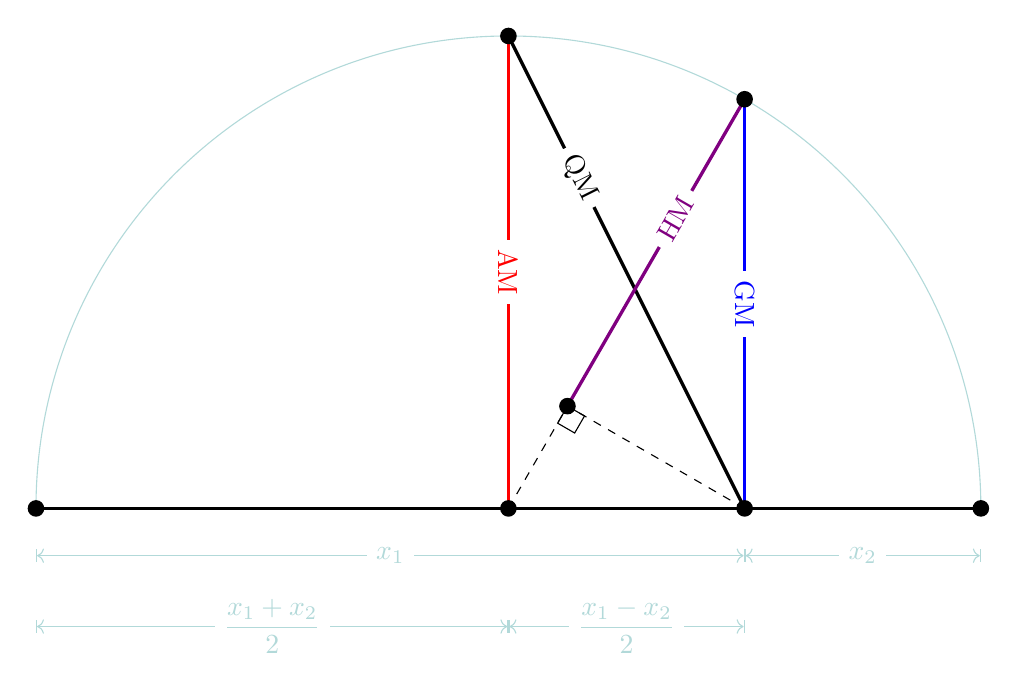
\begin{tikzpicture}[scale=1.0]
    \draw[help lines](-6,0)--(6,0) arc (0:180:6);
    \draw[help lines,|<->|](-6,-0.6)--(3,-0.6) node[midway,fill=white]{$x_1$};
    \draw[help lines,|<->|](3,-0.6)--(6,-0.6) node[midway,fill=white]{$x_2$};
    \draw[help lines,|<->|](-6,-1.5)--(0,-1.5)node[midway,fill=white]{$\dfrac{x_1+x_2}2$};
    \draw[help lines,|<->|](0,-1.5)--(3,-1.5)node[midway,fill=white]{$\dfrac{x_1-x_2}2$};
    \coordinate (G) at (60:6);
    \coordinate (H) at (60:1.5);
    \tkzDefPoint(3,0){C}
    \tkzDefPoint(0,0){O}
    \tkzMarkRightAngle[draw,fill=white](O,H,C)
    \draw[very thick, blue](G)--(C) node[sloped,midway,fill=white]{GM};
    \draw[very thick, red](0,6)--(0,0) node[midway,sloped,fill=white]{AM};
    \draw[very thick](0,6)--(C) node[sloped,pos=0.3,fill=white]{QM};
    \draw[very thick, violet](H)--(G) node[sloped,pos=0.61,fill=white]{HM};
    \draw[very thick](-6,0)--(6,0);
    \fill (-6,0) circle(3pt);
    \fill (C) circle(3pt);
    \fill (6,0) circle(3pt);
    \fill (G) circle(3pt);
    \fill (H) circle(3pt);
    \fill (0,6) circle(3pt);
    \fill (O) circle(3pt);
    \draw[dashed](0,0)--(H);
    \draw[dashed](3,0)--(H);
  \end{tikzpicture}
  \caption{$n=2$时HM,GM,AM,QM的几何示意}
  \label{fig:HM-GM-AM-QM}
\end{figure}

\begin{lemma}\label{lemma:b-1-a}
  若$b\le1\le a$,则$ab\le a+b-1$。
\end{lemma}
\begin{proof}
  由$0\le (a-1)(1-b)=a+b-ab-1$可得。此引理比较重要,被应用到很多不等式的证明过程中。
\end{proof}

\begin{lemma}\label{lemma:product-ai-ge-n}
  $\forall a_i>0$,若满足$\prod_{i=1}^n a_i=1$,则以下不等式成立
  \begin{align}
    \sum_{i=1}^n a_i\ge n
  \end{align}
  当且仅当$a_1=a_2=\cdots=a_n=1$时上述等号成立。
\end{lemma}
\begin{proof}
  对$n$作数学归纳。当$n=1$时显然。当$n\ge2$时,不妨对$a_i$重新排列使得$a_1\equiv\max(a_1,a_2,\cdots,a_n)\ge1$,$a_2\equiv\min(a_1,a_2,\cdots,a_n)\le1$,那么以下$n-1$个数的序列
  \begin{align*}
    a_1a_2, a_3, a_4, \cdots, a_n
  \end{align*}
  满足$n-1$的情况,从而有
  \begin{align*}
    a_1a_2 + a_3+ a_4+ \cdots + a_n &\ge n-1
  \end{align*}
  当且仅当$a_1a_2=a_3=a_4=\cdots=a_n=1$时等号成立,又由引理\ref{lemma:b-1-a},$a_1+a_2 - 1\ge a_1a_2$,其中等号当且仅当$a_1=1$或者$a_2=1$时成立。代入后有
  \begin{align*}
    (a_1 + a_2 - 1) + a_3+ a_4+ \cdots + a_n &\ge n-1\\
    a_1 + a_2 + \cdots + a_n\ge n
  \end{align*}
  其中等号成立,当且仅当以下两个条件同时满足:
  \begin{enumerate}
  \item $a_1a_2=a_3=a_4=\cdots=a_n=1$
  \item $a_1=1$或者$a_2=1$
  \end{enumerate}
  由此条件可知当且仅当所有的$a_i$都等于1时等号成立。
\end{proof}

下面证明AM-GM不等式。
\begin{proof}
  令$g\equiv\sqrt[n]{\prod\limits_{i=1}^n a_i}$,对序列
  \begin{align*}
    \frac{a_1}{g}, \frac{a_2}{g}, \frac{a_3}{g}, \cdots, \frac{a_n}{g}
  \end{align*}
  应用引理\ref{lemma:product-ai-ge-n},有
  \begin{align*}
    \frac{a_1}{g} + \frac{a_2}{g} + \frac{a_3}{g} + \cdots + \frac{a_n}{g}&\ge n\\
    \frac{a_1 + a_2 + a_3 + \cdots + a_n}{n}&\ge g = \sqrt[n]{a_1a_2a_3\cdots a_n} \qedhere
  \end{align*}
\end{proof}

对于三角形,HM还有以下几何意义:
\begin{example}
  对任意三角形,其内切圆的半径是三角形三条高长度的调和平均值的三分之一,即
  \begin{align*}
    r=\frac13 HM(h_a,h_b,h_c)
  \end{align*}
\end{example}
\begin{proof}
  尝试用面积来解,如图~\ref{fig:incircle}所示设三边边长分别是$a,b,c$,
  其对应的高分别为 $h_a, h_b, h_c$,则三角形面积$S=\frac12
  ah_a = \frac12 bh_b = \frac12 ch_c$,同样有$S=\frac12 r(a+b+c)$,从而
  \begin{align*}
    & S = \frac12 r\left( \frac{2S}{h_c} +\frac{2S}{h_a} + \frac{2S}{h_b} \right)
    \quad \implies\quad  r=\frac{1}{\dfrac1{h_a} + \dfrac1{h_b} + \dfrac1{h_c}} \qedhere
  \end{align*}
\end{proof}

\begin{figure}[htbp]
  \centering
  \begin{tikzpicture}[scale=1]
    \tkzDefPoint[label=below left:$A$](0,0){A}
    \tkzDefPoint[label=below right:$B$](6,0){B}
    \tkzDefPoint[label=above:$C$](5,5){C}
    
    \tkzDefCircle[in](A,B,C)\tkzGetPoint{I}\tkzGetLength{rIN}
    \tkzDrawCircle[R](I,\rIN pt);
    \tkzDrawSegments(A,B B,C C,A)
    \tkzDrawSegments[dashed](I,A I,B I,C)
    \tkzDrawCircle[fillstyle=solid,R](I,2pt)

    \coordinate(IA) at ($(B)!(I)!(C)$);
    \coordinate(IB) at ($(C)!(I)!(A)$);
    \coordinate(IC) at ($(A)!(I)!(B)$);

    \tkzDrawSegments[dashed](I,IA I,IB I,IC)
    \tkzMarkRightAngle[color=blue](B,IC,I)
    \tkzMarkRightAngle[color=blue](C,IA,I)
    \tkzMarkRightAngle[color=blue](A,IB,I)
  \end{tikzpicture}
  \caption{三角形内切圆}
  \label{fig:incircle}
\end{figure}

\begin{example}
  若任意非负数$a,b,c$满足$(a+1)(b+1)(c+1)=8$,则$abc\le 1$。
\end{example}
\begin{proof}
  若$a,b,c$均非负,则由AM-GM不等式,有$a+1\ge 2\sqrt{a}$,从而
  \begin{align*}
    8=(a+1)(b+1)(c+1)\ge 2\sqrt{a}\times 2\sqrt{b} \times 2\sqrt{c}
  \end{align*}
  即$abc\le1$。当且仅当$a=b=c=1$时等号成立。
\end{proof}

上述条件不能扩展到任意实数,$a,b,c$一负两正或者三个都是负数,则显然$abc<0$;但对
于$a,b,c$两负一正,比如$a=-2,b=-2,c=7$,则$abc>1$。



\begin{question}\label{q:1/1+a+b}
  三个正数$a,b,c$的乘积是1,求证
  \begin{align*}
    \frac1{1+a+b} + \frac1{1+b+c} + \frac1{1+c+a} \le 1
  \end{align*}
  当且仅当$a=b=c=1$时等号成立。
\end{question}

先尝试猜测每一项的上界。
\begin{align*}
  1+a+b\ge 3\sqrt[3]{ab},\quad 1+b+c \ge 3\sqrt[3]{bc},\quad 1+c+a\ge 3\sqrt[3]{ca}
\end{align*}
从而
\begin{align*}
  \frac1{1+b+c} + \frac1{1+c+a} + \frac1{1+a+b} \le
  \frac13\left( \frac1{\sqrt[3]{ab}} + \frac1{\sqrt[3]{bc}} + \frac1{\sqrt[3]{ca}} \right)
\end{align*}
令$a\to0+, b\to 0+, c=\frac1{ab}$,则上式$\le$符号右边$\to+\infty$,从而没上界,此估计无用。

% 又任意正数$x,y$,有
% \begin{align*}
%   \sqrt{xy}\ge \frac2{\dfrac1x + \dfrac1y}%
%   % \implies  \frac1{xy}\le \frac2{\dfrac1{x^2} + \dfrac1{y^2}}
% \end{align*}

% 令$a_0=\sqrt[6]a, b_0=\sqrt[6]b, c_0=\sqrt[6]c$,代入,有
% \begin{align*}
%   \frac1{\sqrt[3]{ab}} = \frac1{\sqrt{a_0b_0}}\le \frac2{\dfrac1{a_0} + \dfrac1{b_0}}
%   =\frac{2a_0b_0}{a_0+b_0}
% \end{align*}
% 同理处理$\frac1{\sqrt[3]{bc}}$和$\frac1{\sqrt[3]{ca}}$,从而有
% \begin{align*}
%   \frac1{1+b+c} + \frac1{1+c+a} + \frac1{1+a+b} \le
%   \frac23 \left(
%   \frac{a_0b_0}{a_0+b_0} + \frac{b_0c_0}{b_0+c_0} + \frac{c_0a_0}{c_0+a_0} 
%   \right)
% \end{align*}
% 其中$a_0b_0c_0=1$,且上式当且仅当$a_0=b_0=c_0=1$时等号成立。{\color{red}往下似乎不好走了,尝试换个方法。}


\begin{lemma}
对任意$a,b,c\in\mathcal{R}$,有以下恒等式:
\begin{align*}
  (a+b+c)(ab+bc+ca)&=a^2b+a^2c+b^2c+b^2a+c^2a+c^2b + 3abc\\
                   &=(a+b)(b+c)(c+a)+abc
\end{align*}
\end{lemma}
\begin{proof}
  左右分别展开可得证。
\end{proof}

令$x=b+c, y=c+a, z=a+b$,代入有
\begin{align*}
  & \frac1{1+b+c}+\frac1{1+c+a}+\frac1{1+a+b}\le 1\\
  \iff & \underline{(1+x)(1+y)} + (1+y)(1+z) + (1+z)(1+x) \le \underline{(1+x)(1+y)(1+z)}\\
  \iff & \underline{z(1+x)(1+y)} - \underline{(1+y)(1+z)} - (1+z)(1+x) \ge 0\\
  \iff & \underline{zx(1+y)} - (1+y) - 1-x-z-\underline{zx}\ge 0\\
  \iff & zxy - 2 - (x+y+z)\ge 0\\
  \iff & (a+b)(b+c)(c+a) - 2 - 2(a+b+c)\ge 0\\
  \iff & (a+b+c)(ab+bc+ca) - abc -2(a+b+c)\ge 2 \quad(\text{把}abc=1\text{代入})\\
  \iff & (a+b+c)(ab+bc+ca-2)\ge 3
  % \iff & (1+c+a)(1+a+b) + (1+b+c)(1+a+b) + (1+b+c)(1+c+a) \le (1+b+c)(1+c+a)(1+a+b)\\
  % \iff & (b+c)(1+c+a)(1+a+b) - (1+b+c)(1+a+b) - (1+b+c)(1+c+a) \ge 0\\
  % \iff & (b+c)(c+a)(1+a+b) - (1+a+b) - (1+b+c)(1+c+a) \ge 0\\
  % \iff & (b+c)(c+a)(a+b) - (1+a+b) - (1+c+a) - (b+c) \ge 0\\
  % \iff & (b+c)(c+a)(a+b) - 2(1+a+b+c)\ge 0\\
  % \iff & cab+b^2c+a^2b+ab^2 +c^2a+bc^2+a^2c+abc - 2(1+a+b+c)\ge 0\\
  % \iff & b^2c+a^2b+ab^2 +c^2a+bc^2+a^2c - 2(a+b+c)\ge 0\\
  % \iff & (a+b+c)(ab+bc+ca)-3abc -2(a+b+c)\ge 0\\
  % \iff & (a+b+c)(ab+bc+ca-2)\ge 3
\end{align*}
而由AM-GM不等式,有$a+b+c\ge 3\sqrt[3]{abc}=3, ab+bc+ca\ge 3\sqrt[3]{ab\cdot bc\cdot ca}=3$,可得。


\begin{question}
  上题中能否推广到任意正整数$n$,若正数$a_1,a_2,\cdots,a_n$的乘积是$1$,且令$S$表示其和,即
  \begin{align*}
    S\equiv\sum_{i=1}^n a_i
  \end{align*}
  则有
  \begin{align*}
    \sum_{i=1}^n \frac{1}{1 - a_i + S}\le 1
  \end{align*}
  当且仅当$a_1=a_2=\cdots=a_n=1$时等号成立?
\end{question}

当$n=1$时,$a_1=1$,有
\begin{align*}
  \sum_{i=1}^n \frac{1}{1 - a_i + S} = \frac{1}{1} = 1
\end{align*}

当$n=2$时,由$a_1a_2=1$,代入后恒有
\begin{align*}
  \sum_{i=1}^n \frac{1}{1 - a_i + S} &= \frac{1}{1+a_2} + \frac1{1+a_1}\\
                                     &= \frac{1+a_1 + 1 + a_2}{(1+a_1)(1+a_2)}\\
                                     &=1
\end{align*}

当$n=3$时,由题\ref{q:1/1+a+b}已得证。若用引理\ref{lemma:product-ai-ge-n},有$S\ge 3$,从而
\begin{align*}
  \sum_{i=1}^n \frac{1}{1 - a_i + S} &\le \sum_{i=1}^n \frac{1}{1 - a_i + 3}\\
                                     &=   \sum_{i=1}^n \frac{1}{4 - a_i}\\
\end{align*}
{\color{red}上式可不一定,比如$a_i>4$呢?这方法不一定可行。}

用数学归纳法。设$n\le k$时成立,考虑$n=k+1$的情况。考虑数列$\{a_1,a_2,\cdots, a_{k-1}, a_ka_{k+1}\}$,共$k$个数,且其乘积为$1$,从而有
\begin{align*}
  \sum_{i=1}^{k} \frac{1}{1 - a_i' + S_{k+1}'}
\end{align*}
其中
\begin{align*}
  a_i'=
  \begin{cases}
    a_i &i=1,2,\cdots,k-1\\
    a_ka_{k+1} &i=k
  \end{cases} \quad
  S_{k+1}'= a_1+a_2+\cdots +a_{k-1} + a_ka_{k+1}
\end{align*}

%%%%%%%%%%%%%%%%%%%%%%%%%%%%%%%%%%%%%%%%
%%% Basic inequality examples
%%%%%%%%%%%%%%%%%%%%%%%%%%%%%%%%%%%%%%%%
\begin{example}
  证明对$\forall a,b,c\in\mathcal{R}$,有$a^2+b^2+c^2\ge ab+bc+ca$。
\end{example}
\begin{proof}
  由AM--GM不等式,有
\begin{align*}
  a^2+b^2\ge 2ab,\quad b^2+c^2\ge 2bc,\quad c^2+a^2\ge 2ca
\end{align*}
三式相加并除以2可得。该不等式可以推广:$\forall n>1, x_i\in\mathcal{R}(i=1,2,\cdots,n)$,有
\begin{align*}
  \sum_{i=1}^n x_i^2\ge \sum_{i=1}^n x_ix_{i+1}
\end{align*}
其中$x_{n+1}=x_1$。
\end{proof}

\begin{example}
  对任意非负数$a,b$及正整数$n\ge2$,有 $(n-1)a^n + b^n\ge na^{n-1}b$。
\end{example}
对序列$a^n,a^n,\cdots,a^n,b^n$(其中有$n-1$项$a^n$应用AM-GM不等式,有)
\begin{align*}
  \underbrace{a^n + a^n + \cdots + a^n}_{n-1\text{个}} + b^n \ge
  n\times \sqrt[n]{\left(a^n\right)^{n-1} b^n}
  = na^{n-1}b
\end{align*}
当$n=3,4,5$时,有
\begin{align*}
  2a^3 + b^3&\ge 3a^2b\\
  3a^4 + b^4&\ge 4a^3b\\
  4a^5 + b^5&\ge 5a^4b
\end{align*}

\begin{example}
  若正数$a,b,c$的乘积为$1$,求$ab+bc+ca$的极值。
\end{example}
\begin{proof}[提示]
\begin{align*}
  ab+bc+ca\ge 3\times\sqrt[3]{ab\cdot bc\cdot ca}=3\times\sqrt[3]{(abc)^2}=3
\end{align*}
当且仅当$a=b=c=1$时等号成立。另一方面,令$a=b=n,c=1/n^2$,则
\begin{align*}
  ab+bc+ca>ab=n^2\to+\infty (n\to+\infty)
\end{align*}
即$ab+bc+ca$无上界。
\end{proof}


\begin{example}
  若正数$a,b,c$的乘积为$1$,求$a+b+c$的极值。
\end{example}
\begin{align*}
  a+b+c\ge 3\times\sqrt[3]{abc}=3
\end{align*}
当且仅当$a=b=c=1$时等号成立。另一方面,令$a=b=n,c=1/n^2$,则
\begin{align*}
  a+b+c>a=n\to+\infty(n\to+\infty)
\end{align*}
即$a+b+c$无上界。

\begin{example}
  找出所有满足下列等式的实数$a,b,c,d$
  \begin{align*}
    a^2+b^2+c^2+d^2=a(b+c+d)
  \end{align*}
\end{example}

$\forall a,b,c,d\in\mathcal{R}$,有
\begin{align*}
  \left(\frac a2\right)^2\ge 0,\quad \left(\frac a2\right)^2 + b^2\ge ab,
  \quad \left(\frac a2\right)^2 + c^2\ge ac, \quad \left(\frac a2\right)^2 + d^2\ge ad
\end{align*}
四式相加,有
\begin{align*}
  a^2+b^2+c^2+d^2\ge a(b+c+d)
\end{align*}
当且仅当$a=0, \frac a2=b=c=d$时即$a=b=c=d=0$时成立。即原题只有$a=b=c=d=0$这一个解。

\begin{example}
  若正数$a,b,c$的平方和为1,求下式的最小值
  \begin{align*}
    S=\frac{a^2b^2}{c^2} + \frac{b^2c^2}{a^2} + \frac{c^2a^2}{b^2}
  \end{align*}
\end{example}

由
\begin{align*}
  \frac{a^2b^2}{c^2} + \frac{b^2c^2}{a^2}\ge 2b^2,\quad
  \frac{b^2c^2}{a^2} + \frac{c^2a^2}{b^2}\ge 2c^2,\quad
  \frac{c^2a^2}{b^2} + \frac{a^2b^2}{c^2}\ge 2a^2
\end{align*}
三式相加并除以2,有
\begin{align*}
  S\ge a^2+b^2+c^2=1
\end{align*}
当且仅当$\dfrac{a^2b^2}{c^2} = \dfrac{b^2c^2}{a^2} = \dfrac{c^2a^2}{b^2}$即$a=b=c=\frac1{\sqrt3}$时等号成立。


\begin{example}
  $x,y$是小于1的正数,则
  \begin{align*}
    \frac1{1-x^2} + \frac1{1-y^2} \ge \frac2{1-xy}
  \end{align*}
\end{example}
由$x+y\ge2\sqrt{xy}$,有
\begin{align*}
  \frac1{1-x^2} + \frac1{1-y^2} &\ge \frac2{\sqrt{(1-x^2)(1-y^2)}} &&\text{等号成立}\iff x=\pm y\\
  &=\frac2{\sqrt{1+x^2y^2-x^2-y^2}} \\
  &\ge \frac2{\sqrt{1+x^2y^2-2xy}} &&\text{等号成立}\iff x=y\\
  &=\frac2{\sqrt{(1-xy)^2}} \\
  &=\frac2{1-xy}
\end{align*}
当且仅当$x=y$时等号成立。

\begin{example}
  对任意非负数$a,b$,有
  \begin{align*}
    a^3+b^3\ge a^2b+ab^2
  \end{align*}
  推广:对任意非负数$a,b,c$,有
  \begin{align*}
    a^3+b^3+c^3\ge a^2b+b^2c+c^2a
  \end{align*}
  上述结论对任意$n>1$个非负数$a_1,a_2,\cdots,a_n$是否成立,即
  \begin{align*}
    \sum_{i=1}^n a_i^3\ge a_1^2a_2 + a_2^2a_3 + \cdots + a_{n-1}^2a_n + a_n^2a_1
  \end{align*}
\end{example}
由$a^3+b^3-a^2b-ab^2=a^2(a-b)+b^2(b-a)=(a-b)^2(a+b)\ge0$可得,当且仅当$a=b$时等号成立。

由$2a^3+b^3\ge3a^2b$,轮换$a,b,c$,有
\begin{align*}
  2a^3+b^3\ge3a^2b,\quad 2b^3+c^3\ge3b^2c,\quad 2c^3+a^3\ge3c^2a
\end{align*}
三式相加并除以3可得。

\begin{theorem}[Shapiro不等式,Shapiro's Cyclic Inequalities]
  $n$是正整数,序列$\{x_1,x_2,\cdots,x_n\}$是正数序列,则
  \begin{enumerate}
  \item 若$n$是正奇数且$3\le n\le 23$,则
    \begin{align*}
      \sum_{i=1}^{n} \frac{x_i}{x_{i+1} + x_{i+2}} \ge \frac{n}{2}  
    \end{align*}
    其中$x_{n+1} = x_1, x_{n+2} = x_2$。当且仅当$x_1=x_2=\cdots=x_n$时等号成立;

  \item 若$n$且正偶数且$4\le n\le 12$,则
    \begin{align*}
      \sum_{i=1}^{n} \frac{x_i}{x_{i+1} + x_{i+2}} \ge \frac{n}{2}  
    \end{align*}
    当且仅当$x_1=x_3=x_5=\cdots=x_{n-1}$且$x_2=x_4=x_6=\cdots=x_n$时等号成立;

  \item 若$n$是大于12的偶数或者是大于23的奇数,则存在正数序列$\{x_1,x_2,\cdots,x_n\}$,使得
    \begin{align*}
      \sum_{i=1}^{n} \frac{x_i}{x_{i+1} + x_{i+2}} < \frac{n}{2}  
    \end{align*}
  \end{enumerate}
\end{theorem}
\begin{proof}[说明]
  这里仅说明一下其证明历史。B.~A.~Troesch在1989年证明了(1),P.~J.~Bushell \& J.~B.~McLeod在2002年证明了(2),而(3)则是早在1979年就被 J.~L.~Searcy \& B.~A.~Troesch所证明。
\end{proof}

\begin{example}[Nesbitt不等式]
  对任意正数$a,b,c$,有
  \begin{align*}
    \frac{a}{b+c}+\frac{b}{c+a}+\frac{c}{a+b}\ge\frac32
  \end{align*}
\end{example}
\begin{proof}[提示]
  这是Shapiro不等式在$n=3$时的情形。有多种巧妙的证明方法。下面是其中三种。
  \begin{enumerate}
  \item 利用凸函数的Jensen不等式。记$S=a+b+c$,则
    \begin{align*}
      f(x)=\frac{x}{S-x}
    \end{align*}
    在$x\in[0,S)$上是凸的,应用Jensen不等式,则有
    \begin{align*}
      \frac{f(a) + f(b) + f(c)}{3}\ge f\left(\frac{a+b+c}{3}\right)=f\left(\frac{S}{3}\right)=\frac12
    \end{align*}
  \item 用换元法,消除难处理的分母。令$x=a+b,y=b+c,z=c+a$,则$x,y,z$是正数,且有
    \begin{align*}
      a=\frac{x-y+z}2,\quad b=\frac{x+y-z}2,\quad c=\frac{-x+y+z}2
    \end{align*}
    代入,有
    \begin{align*}
      \frac{a}{b+c}+\frac{b}{c+a}+\frac{c}{a+b}
      &= \frac{x-y+z}{2y} + \frac{x+y-z}{2z} + \frac{-x+y+z}{2x}\\
      &= \frac12\left(\frac{x+z}{y} + \frac{x+y}{z} + \frac{y+z}{x}\right)-\frac32\\
      &= \frac12\left( \underbrace{\left(\frac xy + \frac yx\right)}_{\text{应用AM--GM不等式}}
        +\left(\frac zy + \frac yz\right)
        +\left(\frac xz + \frac zx\right)
        \right)-\frac32\\
      &\ge \frac12\times ( 2 + 2 + 2) - \frac32=\frac32
      % &=\frac32
    \end{align*}
    当且仅当$\dfrac xy=\dfrac yx$, $\dfrac zy=\dfrac yz$, $\dfrac xz=\dfrac zx$即$x=y=z$时等号成立,亦即$a=b=c$时等号成立。

  \item 直接利用AM--HM不等式。由
    \begin{align*}
      & \frac{(a+b)+(b+c)+(c+a)}{3}\ge \frac{3}{\dfrac1{a+b}+\dfrac1{b+c}+\dfrac1{c+a}}\\
      \iff & \big[(a+b)+(b+c)+(c+a)\big]\left(\dfrac1{a+b}+\dfrac1{b+c}+\dfrac1{c+a}\right)\ge 9\\
      \iff & 2(a+b+c)\left(\dfrac1{a+b}+\dfrac1{b+c}+\dfrac1{c+a}\right)\ge 9\\
      \iff & 2\left(1+\dfrac{c}{a+b}+1+\dfrac{a}{b+c}+1+\dfrac{b}{c+a}\right)\ge 9
    \end{align*}
    展开可得。其等号成立的充要条件是$a+b=b+c=c+a$,即$a=b=c$。$\qedhere$
  \end{enumerate}
\end{proof}

\begin{question}
  证明Shapiro不等式在$n=4$时的情况,即对任意正数$a,b,c,d$,有
  \begin{align*}
    \frac{a}{b+c}+\frac{b}{c+d}+\frac{c}{d+a}+\frac{d}{a+b}\ge 2
  \end{align*}
\end{question}
% \begin{proof}[提示]
%   应用\ref{lemma:titu}的T2引理,有
%   \begin{align*}
%          &\frac{a}{b+c}+\frac{b}{c+d}+\frac{c}{d+a}+\frac{d}{a+b}\\
%     =\   &\frac{a^2}{a(b+c)}+\frac{b^2}{b(c+d)}+\frac{c^2}{c(d+a)}+\frac{d^2}{d(a+b)}\\
%     \ge\ &\dfrac{(a+b+c+d)^2}{a(b+c) + b(c+d) + c(d+a) + d(a+b)}
%   \end{align*}

%   \begin{align*}
%        & \frac{a}{b+c}+\frac{b}{c+d}+\frac{c}{d+a}+\frac{d}{a+b}\\
%     =\ & \left(\frac{a}{b+c}+\frac{c}{d+a}\right) + \left(\frac{b}{c+d}+\frac{d}{a+b}\right)\\
%     \ge\ & \dfrac{(a+c)^2}{a(b+c)+c(d+a)} + \dfrac{(b+d)^2}{b(c+d)+d(a+b)}\\
%     =\ & \dfrac{a^2+2ac+c^2}{ab+ac+cd+da}
%   \end{align*}
% \end{proof}

% 同样应用换元法简化分母,令$w=a+b$,$x=b+c$,$y=c+d$,$z=d+a$。先反求用$w$,$x$,$y$和$z$表示$a$:
% \begin{enumerate}
% \item 先看$w$,比$a$多了个$b$;
% \item $x$有$b$,$w-x=a-c$,又多减了个$c$;
% \item $y$里有$c$,$w-x+y=a+d$,则又多加了个$d$;
% \item $z$里有$d$,$w-x+y-z=2a$,多加了个$a$。
% \end{enumerate}
% 从而有$a=(w-x+y-z)/2$。类似地,有
% \begin{align*}
%   a&=\frac{w-x+y-z}2 & b&=\frac{x-y+z-w}2\\
%   c&=\frac{y-z+w-x}2 & d&=\frac{z-w+x-y}2
% \end{align*}
% 代入,有
% \begin{align*}
%      &\frac{a}{b+c}+\frac{b}{c+d}+\frac{c}{d+a}+\frac{d}{a+b}\\
%   =\ &\frac{w-x+y-z}{2x} + \frac{x-y+z-w}{2y} + \frac{y-z+w-x}{2z} + \frac{z-w+x-y}{2w}\\
%   =\ &\frac12\left( \frac{w+y-z}{x} + \frac{x+z-w}{y} + \frac{y+w-x}{z} + \frac{z+x-y}{w} - 4\right)
% \end{align*}
% 有负号,不能直接应用AM--GM不等式。代入继续化简,要证明的不等式等价于
% \begin{align*}
%        & \frac12\left( \frac{w+y-z}{x} + \frac{x+z-w}{y} + \frac{y+w-x}{z} + \frac{z+x-y}{w} - 4\right) \ge 2\\
%   \iff & \frac{w+y-z}{x} + \frac{x+z-w}{y} + \frac{y+w-x}{z} + \frac{z+x-y}{w} \ge 8\\
%   \iff & wyz(w+y-z) + xzw(x+z-w) + ywx(y+w-x) + zxy(z+x-y) \ge 8wxyz\\
%   \iff & w^2(yz-xz+xy) + x^2(wz-wy+yz) + y^2(
% \end{align*}


% {\color{red}似乎没用?}


\begin{question}
  证明:对任意正数$a,b,c$,有
  \begin{align*}
    \frac{a^3}{a^2+ab+b^2}+\frac{b^3}{b^2+bc+c^2}+\frac{c^3}{c^2+ca+a^2}
    \ge
    \frac{a+b+c}{3}
  \end{align*}
\end{question}

\begin{question}
  对任意正数$a_1,a_2,\cdots,a_n,b_1,b_2,\cdots,b_n$,有
  \begin{align*}
    \sum_{i=1}^n\frac{a_ib_i}{a_i+b_i}\le
    \frac{\sum\limits_{i=1}^n a_i \cdot \sum\limits_{i=1}^n b_i}
         {\sum\limits_{i=1}^n a_i + \sum\limits_{i=1}^n b_i}
  \end{align*}
\end{question}
对$n$用数学归纳法。

\begin{question}
  若$a_1,a_2,\cdots,a_n,b_1,b_2,\cdots,b_n$是正数,则
  \begin{align*}
    \sum_{i=1}^n \sqrt{a_ib_i}
    \le
    \sqrt{\sum_{i=1}^n a_i \cdot \sum_{i=1}^n b_i}
  \end{align*}
\end{question}
对$n$用数学归纳法。

\begin{question}
  对正数$a,b,c$,证明
  \begin{align*}
    \frac{5a^3-ab^2}{a+b} & \ge 3a^2-b^2\\
    \frac{5a^3-ab^2}{a+b} + \frac{5b^3-bc^2}{b+c} + \frac{5c^3-ca^2}{c+a} & \ge 2(a^2+b^2+c^2)
  \end{align*}
\end{question}
只需证明第一条即可,而第一条又等价于$2a^3+b^3\ge 3a^2b$。

\begin{question}
  对大于$2$的整数$n$,及非负数$x_1,x_2,\cdots,x_n$,若$x_1=0, x_n=1$,则存在整数$j\in[1,2,\cdots,n-1]$,使得
  \begin{align*}
    \left| x_{j-1} - 2x_j + x_{j+1} \right| \ge \frac{4}{n^2}
  \end{align*}
\end{question}
令$x_0=0,x_{n+1}=1$,且对$k=0,1,2,\cdots,n$,令$y_k=x_{k+1}-x_k$,则$y_0=y_n=0$,且$y_0+y_1+y_2+\cdots+y_n=1$。用反证法。假设对所有的$j=1,2,\cdots,n$,不等式不成立,从而有
\begin{align*}
  y_j - y_{j-1} \le \left| y_j-y_{j-1} \right| = \left| x_{j-1} - 2x_j + x_{j+1} \right| < \frac{4}{n^2}
\end{align*}
对$j=1,2,\cdots,k$加起来,则有
\begin{align*}
  y_k&=y_k-y_0=(y_1-y_0) + (y_2-y_1) + \cdots + (y_k-y_{k-1})\\
  &<\underbrace{\frac{4}{n^2}+\frac{4}{n^2}+\cdots+\frac{4}{n^2}}_{k\text{个}}\\
  &=\frac{4k}{n^2}
\end{align*}
同样$y_{j-1}-y_j<\frac{4}{n^2}$,加起来,有
\begin{align*}
  y_k&=y_{k}-y_n=(y_k-y_{k+1})+(y_{k+1}-y_{k+2})+\cdots+(y_{n-1}-y_{n})\\
  &<\underbrace{ \frac{4}{n^2}+\frac{4}{n^2}+\cdots+\frac{4}{n^2}}_{n-k\text{个}}\\
  &=\frac{4(n-k)}{n^2}
\end{align*}

若$n$是奇数,则
\begin{align*}
  1&=y_0+y_1+y_2+\cdots+y_n\\
  &=\left(y_1+y_1+\cdots+y_{\frac{n-1}2}\right)
  + \left(y_{\frac{n+1}2}+y_{\frac{n+1}2+1}+\cdots+y_n\right)\\
  & <\frac4{n^2}\left(
  \left(1+2+\cdots+\frac{n-1}2\right) +
  \left( \left(n-\frac{n+1}2\right) + \left(n-\frac{n+1}2-1\right) + \cdots + 1\right)
  \right)\\
  &=2\cdot\frac4{n^2}\left(1+2+\cdots+\frac{n-1}2\right)\\
  &=\frac8{n^2}\left( \left(1+\frac{n-1}2\right)\cdot\frac{n-1}2\cdot\frac12 \right)\\
  &=\frac{n^2-1}{n^2}<1
\end{align*}
矛盾。

若$n$是偶数,则
\begin{align*}
  1&=y_0+y_1+y_2+\cdots+y_n\\
  &=\left(y_1+y_1+\cdots+y_{\frac{n}2-1}\right)
  + \left(y_{\frac{n}2+1}+y_{\frac{n}2+2}+\cdots+y_n\right)
\end{align*}
剩余略。



\chapter{勾股数}
\label{chap:pythagorean_triples}

\begin{definition}[勾股数]
  若正整数$a,b,c$满足$a^2+b^2=c^2$,则称$a,b,c$为勾股数。
\end{definition}

勾股数也称为毕达哥拉斯三元组(Pythagorean Triples)。常见的勾股数有
\begin{align*}
  (3,4,5),\quad (5,12,13)
\end{align*}

\begin{property}
  $a,b,c$是勾股数,则
  \begin{enumerate}
  \item 若$a,b,c$三者的最大公约数是1,则$a,b,c$两两互质。
  \end{enumerate}
\end{property}

\begin{proof}
  略。
\end{proof}

\begin{definition}[Primitive Pythagorean Triples]
  勾股数$a,b,c$若两两互质,则称$a,b,c$为原始毕达哥拉斯三元组。
\end{definition}

\begin{lemma}
  $\forall n\in\mathcal{Z}^+, 4n+2$不是完全平方数。
\end{lemma}

\begin{proof}
  $4n+2=2(2n+1)$,而$2n+1$是奇数,即$4n+2$的因式分解中2的幂是奇数1,从而$4n+2$不可能是完全平方数。
\end{proof}

\begin{lemma}
  若$(a,b,c)$是原始毕达哥拉斯三元组,则$a,b$必是一奇一偶。
\end{lemma}

\begin{proof}
  首先排除$a,b$都是偶数的情况,否则$c$也是偶数,这样$(a,b,c)$不互质。再次排除$a,b$都是奇数的情况。假如$a,b$都是奇数,则$a^2\equiv b^2\equiv 1(\mod 4)$,从而$c^2\equiv 1 + 1\equiv 2(\mod 4)$不是一个完全平方数,矛盾。
\end{proof}

\begin{theorem}[Euclid's Formula]
  对任意整数$m>n>0$,则以下三元组是Pythagorean三元组
  \begin{align*}
    a=m^2-n^2,\quad b=2mn,\quad c=m^2+n^2
  \end{align*}
\end{theorem}

\begin{proof}
  略。按定义立得。
\end{proof}

\begin{theorem}\label{th:pythagorean-triples}
  若$(a,b,c)$是原始勾股数,且$a$是奇数,$b$是偶数,则存在两个互质且奇偶相反的整数$m>n>0$,使得
  \begin{align*}
    a=m^2-n^2,\quad b=2mn,\quad c=m^2+n^2
  \end{align*}
\end{theorem}

由此定理可知,原始勾股数都可以由Euclid公式生成。

\begin{proof}
  由于$b$是偶数,$a,c$都是奇数,从而$c\pm a$都是偶数,且有
  \begin{align*}
    \left(\frac b2\right)^2 = \frac{c+a}2\times\frac{c-a}2
  \end{align*}
  
  先证明$\dfrac{c\pm a}2$是互质的,否则存在整数$d>1$整除两数的和(等于$c$)与差(等于$a$),从而$c$和$a$有大于1的公约数$d$,与$(a,b,c)$两两互质矛盾。从而存在$m,n\in\mathcal{Z}^+$,使得
  \begin{align*}
    \frac{c+a}2=m^2,\quad \frac{c-a}2=n^2
  \end{align*}
  由上式得到$(a,b,c)$由$m,n$的表达式,后续过程以及请自行补充完整。

  关于$m,n$的奇偶性不同,首先由$m,n$互质排除两者都是偶数;若都是奇数,则由上面的表达式,$(a,b,c)$三者均为偶数,与$(a,b,c)$两两互质矛盾。从而$m,n$奇偶性不同。
\end{proof}


\begin{example}[1965 Putnam Exam.]
  面积的数值是其周长数值的两倍,且边长是整数的直角三角形总共只有3个。
\end{example}

\begin{proof}
  由定理\ref{th:pythagorean-triples},可设满足条件的三角形边长由下式给出
  \begin{align*}
    a = (m^2-n^2)d,\quad b=2mnd,\quad c=(m^2+n^2)d
  \end{align*}
  其中$d$是三边长的最大公约数,$m,n$满足定理\ref{th:pythagorean-triples}中的条件。再由面积的数值是周长数值的两倍,从而有
  \begin{align*}
    \frac12 \times (m^2-n^2)d\times 2mnd & = 2\left( (m^2-n^2)d + 2mnd + (m^2+n^2)d \right)\\
    \implies (m-n)nd & = 4
  \end{align*}
  由于$m-n$是奇数,从而$m-n=1$,又$n$是4的因数可取$1,2,4$,从而$m,n,d$的有以下三种组合
  \begin{align*}
    (2,1,4),\quad (3,2,2),\quad (5,4,1)
  \end{align*}
  此时对应的三角边长分别是
  \begin{align*}
    (12,16,20),\quad (10,24,26),\quad (9,40,41)
  \end{align*}
  即只有上述三种三角形。
\end{proof}

\begin{example}[1975 IMO]
  证明单位圆上任意两点间距离是有理数的点的集合可以有无限个元素。
\end{example}

\hints 令$A=(1,0),B=(-1,0),O$是原点。考虑
\begin{align*}
  \mathcal{P}\equiv\{p:AP=\frac{2(m^2-n^2)}{m^2+n^2}, BP=frac{4mn}{m^2+n^2}
\end{align*}
其中$m,n$满足定理\ref{th:pythagorean-triples},求$\mathcal{P}$中任意两点距离。

\begin{example}[Wiadom. Mat.(1955/56), pp.194-5, Polish]
  求$3^x+4^y=5^z$的所有正整数解。
\end{example}

\begin{proof}
  首先证明$z$是偶数。考虑模3的余数,有
  \begin{align*}
    1 \equiv 0 + 1^y \equiv 3^x + 4^y \equiv 5^z \equiv (-1)^z \tag*{$\pmod 3$}
  \end{align*}
  从而$z$必须是偶数,设$z=2w$,其中$w\in\mathcal{Z}^+$。从而有
  \begin{align*}
    3^x = 5^{2w} - 4^y = \left(5^w\right)^2 - \left(2^y\right)^2 = \left(5^w + 2^y\right)\left(5^w - 2^y\right)
  \end{align*}
  由于$(5^w + 2^y) + (5^w - 2^y) = 2\times 5^w$不能被3整除,从而$5^w + 2^y$和$5^w - 2^y$中有一个不能被3整除,再由上式,可知
  \begin{align*}
    5^w-2^y =1,\quad 5^w+2^y =3^x
  \end{align*}
  上式对3取模,有
  \begin{align*}
    (-1)^w - (-1)^y &= 1 \tag*{$\pmod 3$}\\
    (-1)^w + (-1)^y &= 0 \tag*{$\pmod 3$}\\
  \end{align*}
  从而$w$是奇数,$y$是偶数(请自行考虑)。若$y>2$,则
  \begin{align*}
     5^w\equiv 5^w+2^y \equiv 3^x \equiv 1\text{或者}3 \tag*{$\pmod 8$}
  \end{align*}
  又$w$是奇数,从而存在非负整数$u$,使得$w=2u + 1$,从而有
  \begin{align*}
    5^w \equiv 5^{2u + 1} \equiv 5\times 25^u \equiv 5\times (24 + 1)^u \equiv 5 \tag*{$\pmod 8$}
  \end{align*}
  两个结果矛盾,从而$y=2$。而由$5^w-2^y=1$,有$w=1$,从而$z=2w=2$,$x=2$。
\end{proof}

\section{几何不等式}
\label{sec:geometric-inequality}

\subsection{基本不等式}
\label{sec:basic-geometric-inequality}

\begin{theorem}
  平面上两点间直线段长度最短。
\end{theorem}

\begin{example}
  平面上凸四边形$ABCD$,$M,N$分别是$AD$和$BC$的中点,则
  \begin{align*}
    MN\le\frac{AB+CD}{2}
  \end{align*}
  当且仅当$AB\parallel CD$时等号成立。

  \centering
  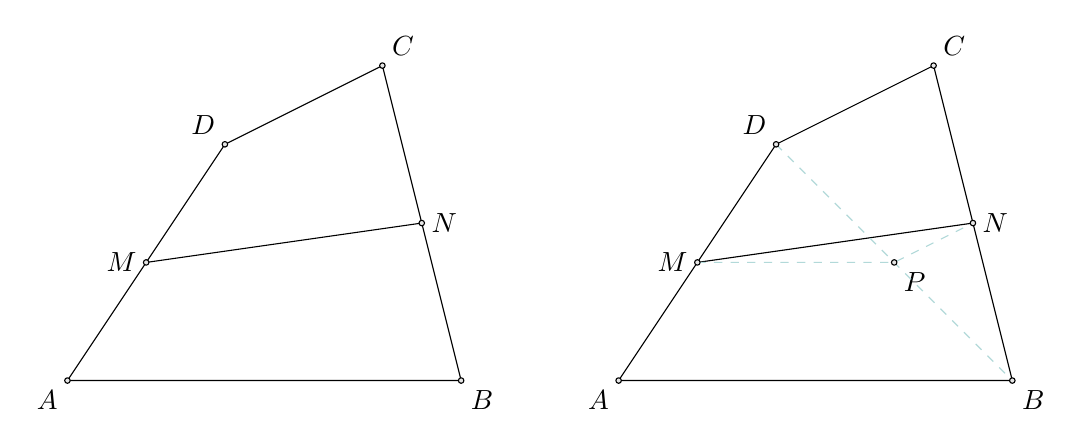
\begin{tikzpicture}[scale=1.0,line join=round]
    \begin{scope}[shift={(0,0)}]
      \coordinate[label=below left:$A$]  (A) at (0,0);
      \coordinate[label=below right:$B$] (B) at (5,0);
      \coordinate[label=above right:$C$] (C) at (4,4);
      \coordinate[label=above left:$D$]  (D) at (2,3);
      \coordinate[label=left:$M$]        (M) at ($.5*(A)+.5*(D)$);
      \coordinate[label=right:$N$]       (N) at ($.5*(B)+.5*(C)$);
      % \coordinate[label=below:$P$] (P) at ($.5*(D)+.5*(B)$);
      \draw(A)--(B)--(C)--(D)--cycle;
      \draw(M)--(N);%--(P)--cycle;
      %\draw(D)--(B);
      \tkzDrawPoints(A,B,C,D,M,N);
    \end{scope}
    \begin{scope}[shift={(7,0)}]
      \coordinate[label=below left:$A$]  (A) at (0,0);
      \coordinate[label=below right:$B$] (B) at (5,0);
      \coordinate[label=above right:$C$] (C) at (4,4);
      \coordinate[label=above left:$D$]  (D) at (2,3);
      \coordinate[label=left:$M$]        (M) at ($.5*(A)+.5*(D)$);
      \coordinate[label=right:$N$]       (N) at ($.5*(B)+.5*(C)$);
      \coordinate[label=below right:$P$] (P) at ($.5*(D)+.5*(B)$);
      \draw(A)--(B)--(C)--(D)--cycle;
      \draw(M)--(N);
      \draw[help lines, dashed](M)--(P)--(N);
      \draw[help lines, dashed](D)--(B);
      \tkzDrawPoints(A,B,C,D,M,N,P);
    \end{scope}
  \end{tikzpicture}
\end{example}
\begin{proof}
  如图取$BD$的点$P$并作辅助线,则
  \begin{align*}
    MN\le MP+NP=\frac{AB+CD}{2}
  \end{align*}
  当且仅当点$P$在$MN$上时等号成立,而$P$在$MN$上时等价于$AB\parallel CD$。
\end{proof}

\begin{theorem}[Pythagorean不等式]
  记三角形的三边分别为$a\le b\le c$,则
  \begin{enumerate}
  \item 三角形是直角三角形$\iff a^2+b^2=c^2$;
  \item 三角形是锐角三角形$\iff a^2+b^2>c^2$;
  \item 三角形是钝角三角形$\iff a^2+b^2<c^2$。
  \end{enumerate}
\end{theorem}
\begin{proof}
  由余弦定理$c^2=a^2+b^2-2ab\cos\mathrm{C}$可得。
\end{proof}


\begin{theorem}[等周不等式,Isoperimetric Inequality]
  若一个平面图形的面积与周长分别为$A$和$P$,则$4\pi A\le P^2$。也就是说在平面上用长度为$P$的线段能围成的最大面积是半径为$\dfrac{P}{2\pi}$的圆,其面积为$\dfrac{P^2}{4\pi}$。
\end{theorem}
\begin{proof}[提示]
  该定理的证明并不平凡,
\end{proof}

\begin{theorem}[三角不等式,Trigonometric Inequality]
  记三角形的三个角分别为$A,B,C$,则
  \begin{align*}
    \sin A +\sin B + \sin C&\le\frac{3\sqrt3}{2}\\
    \cos A +\cos B + \cos C&\le\phantom{3}\,\frac{3}{2}
  \end{align*}
\end{theorem}
\begin{proof}
  由$\sin(x)$及$\cos(x)$在$[0,\pi]$上是凹函数,利用Jensen不等式可得。
\end{proof}

\begin{theorem}[相交弦定理,Intersecting Chords Theorem]
  圆内的两条相交弦,被交点分成的两条线段长的积相等。
\end{theorem}
\begin{proof}
  利用相似三角形可得。
\end{proof}

\begin{theorem}[海伦公式,海伦-秦九韶公式,Heron's Formula]
  记三角形的三边边长分别为$a,b,c$,其半周长$s=\dfrac{a+b+c}2$,则三角形的面积为
  \begin{align}
    S=\sqrt{s(s-a)(s-b)(s-c)}
  \end{align}
\end{theorem}
\begin{proof}
  用余弦公式可证。或者用勾股定理证明$c$边对应的高
  \begin{align*}
    h=\frac{4s(s-a)(s-b)(s-c)}{c^2} &\qedhere
  \end{align*}
\end{proof}

\begin{theorem}
  如图~\ref{fig:r-of-incircle}所示,三角形内切圆将各边分别分割成$x,y,z$的长度,则可得到内切圆的半径公式
  \begin{align}
    r=\sqrt{\frac{xyz}{x+y+z}}=\frac{S}{s}
  \end{align}
\end{theorem}
\begin{figure}[htbp]
  \centering
  \begin{tikzpicture}[scale=1]
    \tkzDefPoint[label=below left:$A$](0,0){A}
    \tkzDefPoint[label=below right:$B$](6,0){B}
    \tkzDefPoint[label=above:$C$](5,5){C}
    
    \tkzDefCircle[in](A,B,C)\tkzGetPoint{I}\tkzGetLength{rIN}
    \tkzDrawCircle[R](I,\rIN pt);
    \tkzDrawSegments(A,B B,C C,A)
    % \tkzDrawSegments[dashed](I,A I,B I,C)

    \coordinate(IA) at ($(B)!(I)!(C)$);
    \coordinate(IB) at ($(C)!(I)!(A)$);
    \coordinate(IC) at ($(A)!(I)!(B)$);

    %\tkzDrawSegments[dashed](I,IA I,IB I,IC)
    \tkzMarkRightAngle[color=blue](B,IC,I)
    \tkzMarkRightAngle[color=blue](C,IA,I)
    \tkzMarkRightAngle[color=blue](A,IB,I)

    \foreach \p in{A,B,C,I,IA,IB,IC}{
      \tkzDrawPoint(\p)
    }
    \tkzLabelPoints[below left](I)

    \draw(A)--(IC) node[below,sloped,midway]{$x$};
    \draw(A)--(IB) node[above left,sloped,midway]{$x$};
    \draw(B)--(IC) node[below,sloped,midway]{$y$};
    \draw(B)--(IA) node[above right,sloped,midway]{$y$};
    \draw(C)--(IB) node[above left,sloped,midway]{$z$};
    \draw(C)--(IA) node[above right,sloped,midway]{$z$};
    \draw[dashed](I)--(IC);
    \draw[dashed](I)--(IA) node[above,sloped,midway]{$r$};
    \draw[dashed](I)--(IB);% node[below left,sloped,midway]{$r$};
  \end{tikzpicture}
  \caption{三角形内切圆的半径}
  \label{fig:r-of-incircle}
\end{figure}
\begin{proof}
  令$s=\dfrac{a+b+c}2$是半周长,则显然有$x=s-a, y=s-b, z=s-c$。由海伦公式可得
  \begin{align*}
    S=\sqrt{xyz(x+y+z)}
  \end{align*}
  另一方面,$S=\dfrac12r(a+b+c)=r(x+y+z)$,从而可得。
\end{proof}

\begin{theorem}[Euler定理]
  记$R,r$分别是三角形的外接圆和内切圆半径,$d$是外接圆与内切圆圆心间的距离,则$d^2=R(R-2r)$,或等价的
  \begin{align*}
    \frac1{R-d}+\frac1{R+d}=\frac1r
  \end{align*}
\end{theorem}
\begin{proof}
  记$G,I$分别是外接圆和内切圆的圆心,在过$G$和$I$的直线上找到长度分别为$R+d$和$R-d$的线段,比如直线$GI$与外接圆的交点$P$、$Q$,则线段$IP$和$IQ$分别为$R\pm d$。

  如图\ref{fig:in/circumcircle},延长$CI$得$L$,延长$LG$得$M$,延长$GI$得$P$和$Q$,则$\triangle CID\sim\triangle MLA$,且$LA=LI$,从而
  \begin{align*}
    (R+d)(R-d)&=IP\cdot IQ=IC\cdot IL=IC\cdot LA=ID\cdot LM=2Rr&\qedhere
  \end{align*}
\end{proof}

\begin{figure}[htbp]
  \centering
%\fbox{%Use \fbox to check the boundary of the tikz picture
  \begin{tikzpicture}[scale=1]
    \tkzDefPoint[label=below left:$A$](0,0){A}
    \tkzDefPoint[label=below right:$B$](6,0){B}
    \tkzDefPoint[label=above:$C$](5,5){C}
    
    \tkzDefCircle[in](A,B,C)\tkzGetPoint{I}\tkzGetLength{rIN}
    \tkzDrawCircle[R](I,\rIN pt);
    \tkzDrawSegments(A,B B,C C,A)
    % \tkzDrawSegments[dashed](I,A I,B I,C)

    % \coordinate(IA) at ($(B)!(I)!(C)$);
    \coordinate[label=above left:$D$](IB) at ($(C)!(I)!(A)$);
    % \coordinate(IC) at ($(A)!(I)!(B)$);

    % \tkzDrawSegments[dashed](I,IA I,IB I,IC)
    \tkzDrawSegments[dashed](I,IB)
    % \tkzMarkRightAngle[color=blue](B,IC,I)
    % \tkzMarkRightAngle[color=blue](C,IA,I)
    \tkzMarkRightAngle[color=blue](A,IB,I)

    % circumcircle
    \tkzCircumCenter(A,B,C)\tkzGetPoint{G}
    \tkzDrawCircle(G,A)
    \tkzInterLC(G,I)(G,A)\tkzGetPoints{P}{Q}

    \draw[dashed](A)--(I);
    \draw[dashed](I)--(P);
    \draw[dashed](I)--(Q);
    \draw[thick](G)--(I);

    \tkzInterLC(C,I)(G,A)\tkzGetPoints{}{L}
    \tkzInterLC(L,G)(G,A)\tkzGetPoints{}{M}

    \tkzLabelPoints[left](P)
    \tkzLabelPoints[right](Q,I)
    \tkzLabelPoints[below](L)
    \tkzLabelPoints[below left](G)
    \tkzLabelPoints[above](M)

    \draw[dashed](C)--(L)--(M)--(A)--(L);

    \foreach \p in{A,B,C,I,G,P,Q,IB,L,M}{
      \tkzDrawPoint(\p)
    }

    % emphasize similar triangles
    \draw[very thick](C)--(I)--(IB)--cycle;
    \draw[very thick](M)--(A)--(L)--cycle;
  \end{tikzpicture}
%}
  % Maybe due to BUG of pgfplots, there're wide space between figure
  % and caption, -3cm is measured by eye
  \vspace*{-3cm}
  \caption{三角形的外接圆与内切圆}
  \label{fig:in/circumcircle}
\end{figure}


\begin{theorem}[Euler不等式]
  记$R,r$分别是三角形$\triangle ABC$的外接圆和内切圆半径,则有$R\ge2r$。
\end{theorem}
\begin{proof}
  由Euler定理立得。
\end{proof}

\begin{theorem}\label{th:R-of-circumcircle}
  任意$\triangle ABC$,其三边边长分别为$a,b,c$,面积为$S$,则其外接圆半径为
  \begin{align}
    R=\frac{abc}{4S}
  \end{align}
\end{theorem}
\begin{figure}[htbp]
  \centering
  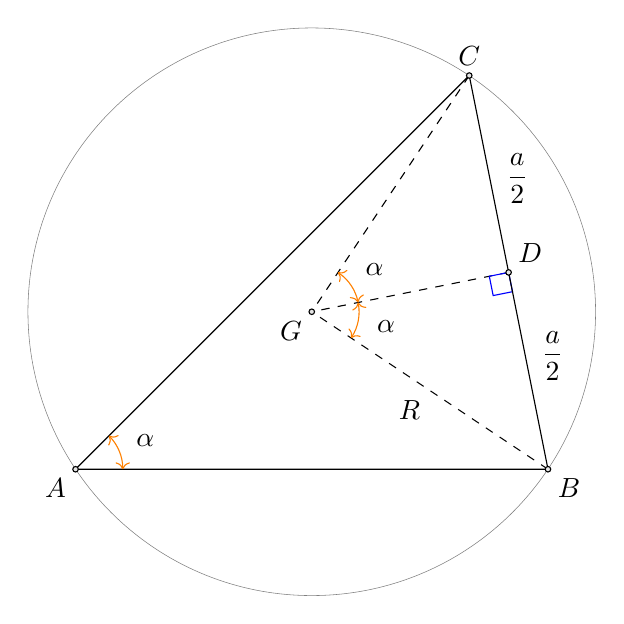
\begin{tikzpicture}[scale=1]
    \tkzDefPoint[label=below left:$A$](0,0){A}
    \tkzDefPoint[label=below right:$B$](6,0){B}
    \tkzDefPoint[label=above:$C$](5,5){C}
    
    % circumcircle
    \tkzCircumCenter(A,B,C)\tkzGetPoint{G}
    \tkzDrawCircle(G,A)
    \tkzLabelPoints[below left](G)

    \coordinate[label=above right:$D$](D) at ($(B)!(G)!(C)$);

    \draw[dashed](B)--(G) node[midway,below left]{$R$};
    \draw[dashed](C)--(G);
    \draw[dashed](D)--(G);
    \tkzMarkRightAngle[color=blue](G,D,B)
    \draw(A)--(B)--(C)
        node[pos=0.20,above right]{$\dfrac{a}2$} 
        node[pos=0.65,above right]{$\dfrac{a}2$} --cycle;

    \draw pic["$\alpha$",draw=orange,<->,angle eccentricity=1.6,angle radius=.6cm] {angle=B--A--C};
    \draw pic["$\alpha$",draw=orange,<->,angle eccentricity=1.6,angle radius=.6cm] {angle=B--G--D};
    \draw pic["$\alpha$",draw=orange,<->,angle eccentricity=1.6,angle radius=.6cm] {angle=D--G--C};

    \foreach \p in{A,B,C,D,G}{
      \tkzDrawPoint(\p)
    }
  \end{tikzpicture}    
  % Maybe due to BUG of pgfplots, there're wide space between figure
  % and caption, -3cm is measured by eye
  \vspace*{-3.5cm}
  \caption{三角形外接圆半径}
  \label{fig:R-of-circumcircle}
\end{figure}
\begin{proof}
  由图~\ref{fig:R-of-circumcircle}容易看出$\angle BAC = \angle CGD = \angle BGD$,从而有
  \begin{align*}
    S_{\triangle ABC} = \frac12 bc\cdot\sin\angle BAC
    = \frac12 bc \cdot \frac{a/2}{R} = \frac{abc}{4R}
  \end{align*}
  从而可算出$R$。
\end{proof}


\begin{theorem}
  任意$\triangle ABC$,记$a,b,c$是其三边边长,$r,R$分别是其内切圆与外接圆半径,则
  \begin{align}
    rR=\frac{abc}{2(a+b+c)}
  \end{align}
\end{theorem}
\begin{proof}
  在定理~\ref{th:R-of-circumcircle},将$r=\dfrac{S}{s}$及$a+b+c=2s$代入可得。
\end{proof}




\begin{theorem}[托勒密不等式,Ptolemy's Inequality]
  任意凸四边形$ABCD$,有
  \begin{align}
    AB\cdot CD + AD\cdot BC\ge AC\cdot BD
  \end{align}
  当且仅当$ABCD$是圆内接四边形等号成立。
\end{theorem}
\begin{proof}
  \color{red}不会呢。
\end{proof}

\begin{theorem}[鄂尔多斯—门德尔不等式,Erdos-Mordell Inequality,E-M不等式]
  $P$是三角形$ABC$内任意一点,$P$到三角形三边的距离分别为$p,q,r$,到三顶点的距离分别是$x,y,z$,则
  \begin{align}
    x+y+z\ge 2(p+q+r)
  \end{align}
\end{theorem}
\begin{proof}
  \color{red}不会呢。
\end{proof}

\section{Cauchy-Schwarz不等式}
\label{sec:cauchy-schwarz-inequalities}

% Cauchy-Schwarz
\begin{theorem}[Cauchy-Schwarz Inequality]
对 $\forall a_i, b_i\in \mathcal{R}$, $\forall n\in\mathcal{Z}^+$, 总有
\begin{align}
  \left(\sum_{i=1}^{n} a_ib_i\right)^2 \le \left(\sum_{i=1}^{n}a_i^2\right) \left(\sum_{i=1}^{n}b_i^2\right)
\end{align}
\end{theorem}

\begin{proof}
  令
  \begin{align*}
    S_n = \left(\sum_{i=1}^{n}a_i^2\right) \left(\sum_{i=1}^{n}b_i^2\right) - \left(\sum_{i=1}^{n} a_ib_i\right)^2
  \end{align*}
  则 $S_1 = a_1^2b_1^2 - (a_1b_1)^2 = 0$,且
  \begin{align*}
    S_{n+1} - S_n =& \phantom{-} \left(\sum_{i=1}^{n+1}a_i^2\right) \left(\sum_{i=1}^{n+1}b_i^2\right) - \left(\sum_{i=1}^{n+1} a_ib_i\right)^2 \\
     &- \left(\sum_{i=1}^{n}a_i^2\right) \left(\sum_{i=1}^{n}b_i^2\right) + \left(\sum_{i=1}^{n} a_ib_i\right)^2\\
  \end{align*}
  请自行证明 $S_{n+1}\ge S_n$。从而有 $S_{n+1}\ge S_n\ge\cdots S_1 = 0$。
\end{proof}

\note 令$A\equiv\left(\sum_{i=1}^{n}a_i^2\right)$, $B\equiv\left(\sum_{i=1}^{n}b_i^2\right)$,$C\equiv\left(\sum_{i=1}^{n}b_i^2\right)$,则
\begingroup\allowdisplaybreaks
\begin{align*}
  S_{n+1} - S_n &=&& (A+a_{n+1}^2)(B+b_{n+1}^2) - (C+a_{n+1}b_{n+1})^2 - AB + C^2\\
  &=&& AB + Ab_{n+1}^2 + a_{n+1}^2B + a_{n+1}^2b_{n+1}^2 - C^2 - 2a_{n+1}b_{n+1}C - a_{n+1}^2b_{n+1}^2\\
  &&&- AB + C^2\\
  &=&& Ab_{n+1}^2 + a_{n+1}^2B - 2a_{n+1}b_{n+1}C\\
  &=&& \left(\sum_{i=1}^{n}a_i^2\right) b_{n+1}^2 + \left(\sum_{i=1}^{n}b_i^2\right) a_{n+1}^2
       - \left(\sum_{i=1}^{n}a_ib_i\right) \cdot 2a_{n+1}b_{n+1}\\
  &=&& \sum_{i=1}^{n} \left( a_i^2b_{n+1}^2 + b_i^2a_{n+1}^2 - a_ib_i\cdot 2a_{n+1}b_{n+1} \right)\\
  &=&& \sum_{i=1}^{n} \left( (a_ib_{n+1})^2 + (b_ia_{n+1})^2 - 2(a_ib_{n+1})(b_ia_{n+1}) \right)\\
  &=&& \sum_{i=1}^{n} \left( (a_ib_{n+1} - b_ia_{n+1})^2 \right)\\
  &\ge&&0
\end{align*}
\endgroup


% Convex
\chapter{凸函数}
\label{chap:convex-functions}

一般英文中用Convex function和Concave function来表示凸函数与凹函数。此概念刚传入国内时,convex function被翻译为“下凹函数”,concave function被翻译成“上凸函数”,后来有些作者将其中的“下”与“上”去掉了,convex function就变成了“凹函数”,concave function就变成了“凸函数”,概念完全相反了。这就导致了有相当多的书籍中的凹凸性与concave/convex两字的含议完全相反。若阅读到此类书籍,务必要小心其定义。

%%% 未考证:
% 若你接触到经济学中的凹凸性,则可能又与数学上的定义有差别,这是因为其考虑方向不一样。数学的凹凸性是相对于$x$轴,经济学的凹凸性是相对于原点。

这里取convex/concave两词的本义,即将文献中convex function对应的称为凸函数,concave function对应的称为凹函数。

\section{凸函数的定义}
\label{sec:definition-of-convexity}

\begin{definition}[凸函数,Convex Function]\mbox{}\par
  \begin{enumerate}
  \item 函数$f(x)$被称为域$\mathcal{D}$上的凸函数,若$\forall x1,x2\in\mathcal{D}, t\in[0,1]$,下面不等式成立:
    \begin{align}\label{eq:convex-defintion}
      f\left(tx_1+(1-t)x_2\right)\le tf(x_1) + (1-t)f(x_2)
    \end{align}
  \item 函数$f(x)$被称为域$\mathcal{D}$上的严格凸函数,若$\forall x1,x2\in\mathcal{D}, t\in(0,1),x_1\ne x_2$,下面不等式成立:
    \begin{align}
      f\left(tx_1+(1-t)x_2\right)< tf(x_1) + (1-t)f(x_2)
    \end{align}
  \end{enumerate}
\end{definition}

从图形上看,凸函数对应的曲线上任意两点的连线在曲线之上。令$t\equiv 1-\lambda$代入,不等式\ref{eq:convex-defintion}还可以等价的写成以下形式
\begin{align*}
  f\left(x_1+\lambda(x_2-x_1)\right)\le f(x_1) + \lambda \left(f(x_2)-f(x_1)\right)
\end{align*}


\begin{figure}[htb]
  \centering
  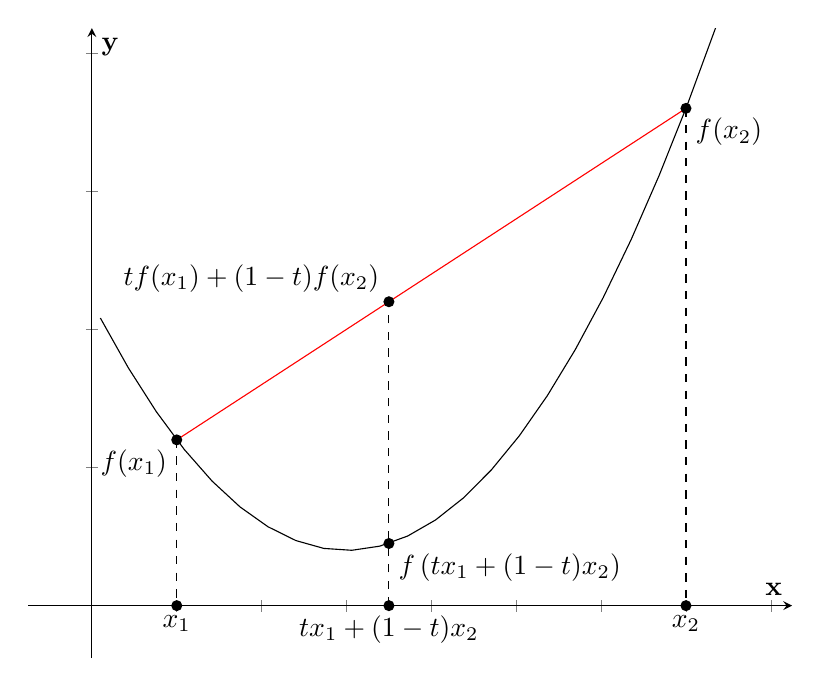
\begin{tikzpicture}[scale=1]
    \begin{axis}[
      scale only axis,
      width=0.8\textwidth,
      height=8cm,
      xmin = 0,
      xmax = 75,
      ymin = 0,
      ymax = 38, 
      axis lines = middle,
      enlargelimits = true,
      xlabel = {$\mathbf{x}$},
      ylabel = {$\mathbf{y}$},
      yticklabels={,,},
      xticklabels={,,}
      ]
      % \addplot+[mark = none] coordinates {%
      %   (0 ,40) 
      %   (20, 30)
      %   (30, 20)
      %   (35, 10)
      %   (39, 0)};
      \coordinate (A) at (axis cs:10,12);
      \coordinate (B) at (axis cs:70,36);
      \coordinate (C) at (axis cs:35,4.5);
      \coordinate (D) at (axis cs:35,22);
      \coordinate (E) at (axis cs:35,0);
      \coordinate (F) at (axis cs:10,0);
      \coordinate (G) at (axis cs:70,0);
      \addplot[domain=1:80] (\x, {0.02 * (\x * \x - 60 * \x + 900) + 4});
      \addplot[dashed](35,0)--(D);
      % \addplot[dashed](A)--(F);
      % \addplot[dashed](B)--(G);
    \end{axis}
    \draw[color=red](A)--(B);
    \fill(A) circle(2pt) node[below left] {$f(x_1)$};
    \fill(B) circle(2pt) node[below right] {$f(x_2)$};
    \fill(C) circle(2pt) node[below right] {$f\left(tx_1 + (1-t)x_2\right)$};
    \fill(D) circle(2pt) node[above left] {$tf(x_1) + (1-t)f(x_2)$};
    \fill(E) circle(2pt) node[below] {$tx_1 + (1-t)x_2$};
    \fill(F) circle(2pt) node[below] {$x_1$};
    \fill(G) circle(2pt) node[below] {$x_2$};
    \draw[dashed](A)--(F);
    \draw[dashed](B)--(G);
  \end{tikzpicture}
  \caption{凸函数}
  \label{fig:convex-function}
\end{figure}

\begin{theorem}
  若$f(x)$在$\mathcal{D}$上二次可导,那么以下条件相互等价:
  \begin{enumerate}
  \item \label{item:convex-1} $f(x)$是凸函数。
  \item \label{item:convex-2} $\forall x,y\in\mathcal{D}, f(y)\ge f(x)+f'(x)(y-x).$
  \item \label{item:convex-3} $\forall x\in\mathcal{D}, f''(x)\ge 0.$
  \end{enumerate}
\end{theorem}
\begin{proof}
  \begin{enumerate}
  \item \ref{item:convex-1}$\implies$\ref{item:convex-2}. 由于$f(x)$是凸函数,从而$\forall\lambda\in(0,1)$,有
    \begin{align*}
      &f\left(x+\lambda(y-x)\right)\le f(x)+\lambda\left(f(y)-f(x)\right)\\
      \implies & f(y)-f(x)\ge \frac{f\left(x+\lambda(y-x)\right) -  f(x)}{\lambda}\\
      \implies & f(y)-f(x)\ge \frac{f\left(x+\lambda(y-x)\right) -  f(x)}{\lambda(y-x)}\cdot(y-x)
    \end{align*}
    上式中令$\lambda\downarrow 0$,即$\Delta x\equiv\lambda(y-x)\downarrow 0$,从而有
    \begin{align*}
      f(y)-f(x)\ge \lim_{\Delta\downarrow 0}\frac{f(x+\Delta x) -  f(x)}{\Delta x}\cdot(y-x) = f'(x)(y-x)
    \end{align*}
  \item \ref{item:convex-2}$\implies$\ref{item:convex-3}.\think 请利用二阶导数定义自行证明。
  \item \ref{item:convex-3}$\implies$\ref{item:convex-1}.\think 利用中值定理自行证明。
  \end{enumerate}
  \note
  其中第\ref{item:convex-2}点说明$f$的曲线在定义域上任意一点的切线之上,
  如图~\ref{fig:convex-function-above-tangent-line}所示;
  第\ref{item:convex-3}点说明曲线的二阶导数非负,也就时说其一阶导数是单
  调增函数。
\end{proof}

\begin{figure}[htb]
  \centering
  \begin{tikzpicture}[scale=1]
    \begin{axis}[
      scale only axis,
      width=0.8\textwidth,
      height=3cm,
      xmin = 0,
      xmax = 75,
      ymin = 0,
      ymax = 27, 
      axis lines = middle,
      enlargelimits = true,
      xlabel = {$\mathbf{x}$},
      ylabel = {$\mathbf{y}$},
      yticklabels={,,},
      xticklabels={,,}
      ]
      \coordinate (A) at (axis cs:40,6);
      \addplot[domain=1:80] (\x, {0.02 * (\x * \x - 60 * \x + 900) + 4});
      \addplot[domain=10:60,color=red] (\x, {6 + 0.4 * (\x - 40)});
    \end{axis}
    \fill(A) circle(2pt) node[below left] {};
  \end{tikzpicture}
  \caption{凸函数示意:曲线位于任一点的切线之上}
  \label{fig:convex-function-above-tangent-line}
\end{figure}


% Jensen
\begin{theorem}
  如果$f(x)$是凸函数,那么对于$p_i\ge0$且$\sum_{i=1}^{n}p_i=1$,有
  \begin{align}
    f(\sum_{i=1}^{n}p_ix_i)\le \sum_{i=1}^{n}p_i f(x_i)
  \end{align}
\end{theorem}

\begin{proof}
  事实上,Jensen不等式与凸函数的定义是等价的,即若函数$f(x)$是凸函数,
  当且仅当$f(x)$满足Jensen不等式。
  \begin{enumerate}
  \item 充分性。在Jensen不等式中令$n=2$,可知$f(x)$满足凸函数定义,从而是凸函数。
  \item 必要性。设$f(x)$是凸函数,$n=2$时Jensen不等式即是凸函数定义中的条件,即Jensen不等式在$n=2$时成立。
    设Jensen不等式对$n\le K$时成立,考虑$n=K+1$的情况。关键点,把其中两项凑成一项,从而$K+1$项变成$K$项,可利用$n\le K$时成立的结论。令
    \begin{align*}
      p_K'&\equiv p_K+p_{K+1}\\
      x_K'&\equiv\frac{p_K}{p_K'}x_K + \frac{p_{K+1}}{p_K'}x_{K+1}\in[\min{(x_K, x_{K+1})}, \max{(x_K, x_{K+1})}]
    \end{align*}
    则有$p_K'x_K' = p_Kx_K + p_{K+1}x_{K+1}$,且
    \begin{align*}
      f\left(\sum_{i=1}^{K+1}p_ix_i\right) &= f\left(\sum_{i=1}^{K-1}p_ix_i  + p_K'x_K'\right)\\
      &\le \left(\sum_{i=1}^{K-1}p_if(x_i)\right) + p_K' f(x_K')\\
      &\le \left(\sum_{i=1}^{K-1}p_if(x_i)\right) + p_K'\left( \frac{p_K}{p_K'}f(x_K) + \frac{p_{K+1}}{p_K'}f(x_{K+1}) \right) \\
      &= \left(\sum_{i=1}^{K+1}p_i f(x_i)\right)
    \end{align*}
    此处没有考虑$p_K'=0$的情况,请自行补充完整。
  \end{enumerate}
  
  \note $p_K'$和$x_K'$是如何凑出来的?令$p_K'x_K' = p_Kx_K + p_{K+1}x_{K+1}$,
  且$p_K'$需满足$\sum_{i=1}^{K-1}p_i + p_K'=1$,从而可得。
\end{proof}

{\color{red}下面这个是对的吗?}
\begin{theorem}
  $f(x)$是$\mathcal{D}$上的严格凸函数,当且仅当对$\forall n\in\mathcal{Z}^+, x_i\in\mathcal{D}, p_i>0, \sum_{i=1}^{n}p_i=1$,以下不等式成立:
  \begin{align*}
    f\left(\sum_{i=1}^{n} p_i x_i\right) < \sum_{i=1}^{n} p_i f(x_i)
  \end{align*}
\end{theorem}


\begin{lemma}\label{lemma:convexity-extension}
  若$f(x)$是$[a,b]$上的连续函数,且在$(a,b]$上是凸的,则$f(x)$在$[a,b]$上是凸函数。
\end{lemma}
\begin{proof}
  下面按定义证明,即$\forall x_1,x_2\in[a,b], 0\le t\le1$,需要证明
  \begin{align*}
    f\left(tx_1 + (1-t)x_2\right) \le tf(x_1) + (1-t)f(x_2)
  \end{align*}
  若$x_1$和$x_2$都不等于$a$,那么由条件$f(x)$在$(a,b]$上严格凸可知上面不等式成立。下面不妨设$a=x_1<x_2\le b$。由连续性,可取到序列$c_i$,使得$\forall i, a=x_1<c_i\le b$,且$\lim c_i = x_1$,从而对于$c_i$和$x_2$,有
  \begin{align*}
    f\left(tc_i + (1-t)x_2\right) \le tf(c_i) + (1-t)f(x_2)
  \end{align*}
  上式中两边对$i$取极限,并由$f(x)$的连续性,有
  \begin{align*}
    \lim_{i\to\infty}f\left(tc_i + (1-t)x_2\right) &\le \lim_{i\to\infty} tf(c_i) + (1-t)f(x_2)\\
    f\left(\lim_{i\to\infty}\left(tc_i + (1-t)x_2\right)\right) &\le tf( \lim_{i\to\infty} c_i) + (1-t)f(x_2)\\
    f\left(tx_1 + (1-t)x_2\right) &\le tf(x_1) + (1-t)f(x_2)
  \end{align*}
\end{proof}

\think 上面引理对严格凸函数是否还能保持严格凸性?

\begin{lemma}\label{lemma:convexity-of-power-function}
  对$p>1$,函数$f(x)\equiv\left|x\right|^p$在$x\in\mathcal{R}$上是严格凸函数。
\end{lemma}
\begin{proof}
  函数$f(x)\equiv|x|^p$的凹凸性在图形上看是非常明显的。

  使用导数的概念证明也是非常明显的,分段考虑,$\forall x>0, f'(x) = p\left|x\right|^{p-1}>0, f''(x)=p(p-1)\left|x\right|^{(p-1)(p-2)}>0$,从而$f(x)$的一阶导数是严格单调递增的,从而$f(x)$在$(0,+\infty)$上是凸函数。同样$f(x)$在$(-\infty,0)$上也是凸函数。

  下面是初等数学的证明。

  $\forall x_1\le x_2, t\in(0,1)$,有
  \begin{align*}
    f\left(tx_1 + (1-t)x_2\right) = \left|tx_1 + (1-t)x_2\right|^p
  \end{align*}
  {\color{red}然后呢??}
\end{proof}

下面是Jensen不等式的另一种形式。
\begin{theorem}[Jensen不等式]
  若$f$是$\mathcal{D}$上的凸函数,且$\forall x_1,x_2,\cdots,x_n\in\mathcal{D}$,则
  \begin{align}
    f\left(\frac{x_1+x_2+\cdots+x_n}{n}\right)\le\frac{f(x_1)+f(x_2)+\cdots+f(x_n)}{n}
  \end{align}
  若$f$还是严格凸的,则当且仅当$x_1=x_2=\cdots=x_n$时等号成立。
\end{theorem}

\begin{proof}
  {\color{red}请证明两种形式的Jensen不等式是等价的。}
\end{proof}

\begin{example}
  对$\triangle ABC$,证明:
  \begin{align*}
    \sin A + \sin B + \sin C \le \frac{3\sqrt3}{2}
  \end{align*}
  且说明等号在何时成立。
\end{example}

\begin{proof}
  $f(x)\equiv\sin(x)$在$[0,\pi]$上是严格凹函数,由Jensen不等式有
  \begin{align*}
    \sin A + \sin B + \sin C \le 3\sin\frac{A+B+C}{3} = \frac{3\sqrt3}{2}
  \end{align*}
  当且仅当$A=B=C$时,即$A=B=C=\frac\pi3$时等号成立。
\end{proof}

\begin{example}
  若$a,b,c$是和为1的正数,求下式的最小值
  \begin{align*}
    \left(a+\frac1a\right)^{10} + 
    \left(b+\frac1b\right)^{10} + 
    \left(c+\frac1c\right)^{10}
  \end{align*}
\end{example}

\begin{proof}
  首先证明以下函数在$(0,1)$上是严格凸函数({\color{red}请用二次导数自行证明})
  \begin{align*}
    f(x)\equiv\left(x+\frac1x\right)^{10}
  \end{align*}
  其次利用Jensen不等式,有
  \begin{align*}
    &\left(a+\frac1a\right)^{10} + 
    \left(b+\frac1b\right)^{10} + 
    \left(c+\frac1c\right)^{10}\\
    ={}  & f(a) + f(b) + f(c)\\
    \ge{}& 3f\left(\frac{a+b+c}3\right)\\
    ={}  & 3f\left(\frac\13\right) = 3 \left(\frac{10}{3}\right)^{10} = \frac{10^{10}}{3^9}
  \end{align*}
  当且仅当$a=b=c=\frac13$时等号成立。
\end{proof}
% Minkowski Inequality

\chapter{Minkowski不等式}
\label{chap:minkowski-inequality}


\begin{theorem}[Minkowski不等式]
  $\forall p\ge 1$以下不等式对任意$x_i,y_i\in\mathcal{R}$成立:
  \begin{align}
    \left(\sum_{i=1}^{n}\left|x_i+y_i\right|^p\right)^\frac{1}{p}
    \le
    \left(\sum_{i=1}^{n}\left|x_i\right|^p\right)^\frac{1}{p}
    +
    \left(\sum_{i=1}^{n}\left|y_i\right|^p\right)^\frac{1}{p}
  \end{align}
  当且仅当存在不同时为零的常数$\alpha,\beta$,$\alpha x_i=\beta
  y_i$对$\forall i\in\{1,2,\cdots,n\}$都成立时等号成立。即若记
  \begin{align*}
    \vec{x}&\equiv\left[x_1,x_2,\cdots,x_n\right]\\
    \vec{y}&\equiv\left[y_1,y_2,\cdots,y_n\right]
  \end{align*}
  则当且仅当 $\vec{x}$ 和 $\vec{y}$ 线性相关时等号成立。
\end{theorem}

Minkowski不等式与函数的凸性相关。

\begin{proof}
  当$p=1$时显然不等式成立。下面考虑$p>1$的情况。由引理\ref{lemma:convexity-of-power-function},$|x|^p$是凸函数,$|x|^{\frac{1}{p}}$是凹函数,从而$\forall t\in(0,1)$,有
  \begin{align*}
    \left|x_i + y_i\right|^p &= \left|t\cdot\frac{x_i}{t} + (1-t)\cdot\frac{y_i}{1-t}\right|^p & \forall t\in (0,1)\\
    &\le t \left|\frac{x_i}{t}\right|^p + (1-t)\left|\frac{y_i}{1-t}\right|^p \\
    &= t^{1-p}|x_i|^p + (1-t)^{1-p}|y_i|^p
  \end{align*}
  求和,则有
  \begin{align*}
    \sum_{i=1}^{n}\left|x_i+y_i\right|^p \le
    t^{1-p}\sum_{i=1}^{n}|x_i|^p + (1-t)^{1-p}\sum_{i=1}^{n}|y_i|^p
  \end{align*}
  记
  \begin{align*}
    \norm{X}  \equiv\left(\sum_{i=1}^{n} |x_i|^p\right)^{\frac1p},\quad
    \norm{Y}  \equiv\left(\sum_{i=1}^{n} |y_i|^p\right)^{\frac1p},\quad
    \norm{X+Y}\equiv\left(\sum_{i=1}^{n} |x_i+y_i|^p\right)^{\frac1p}
  \end{align*}
  并令$t\equiv\frac{\norm{X}}{\norm{X}+\norm{Y}}$(显然 $t\in[0,1]$ 。
  若$t=0$或者$t=1$,则$\norm{X}=0$或者$\norm{Y}=0$,从而Minkowski等号成
  立,所以下面只考虑$t\in(0,1)$的情况),代入则有
  \begin{align*}
    \norm{X + Y}^p &= \sum_{i=1}^{n}\left|x_i+y_i\right|^p\\
    &\le t^{1-p}\sum_{i=1}^{n}|x_i|^p + (1-t)^{1-p}\sum_{i=1}^{n}|y_i|^p\\
    &= \left(\frac{\norm{X}}{\norm{X}+\norm{Y}}\right)^{1-p} \norm{X}^p +
      \left(\frac{\norm{Y}}{\norm{X}+\norm{Y}}\right)^{1-p} \norm{Y}^p\\
    &=\frac{\norm{X}+\norm{Y}}{\left(\norm{X}+\norm{Y}\right)^{1-p}}\\
    &= \left(\norm{X}+\norm{Y}\right)^{p}
  \end{align*}
  从而有$\norm{X+Y}\le\norm{X}+\norm{Y}$,即Minkowski不等式成立。
\end{proof}


\chapter{无字证明}
\label{chap:proofs-without-words}

\epigraph{一图胜千言,一表胜万卷。}{}

无字证明(Proof without Words)是指仅用图像而无需文字解释就能不证自明的数学命题。然而无字证明并不是严格的数学证明,只是帮助直观理解。

\section{代数}
\label{sec:pww-algebra}

\begin{example}
  前$n$个奇数的和等于$n^2$,即
  \begin{align}
    \underbrace{1 + 3 + 5 + \cdots + (2n-1)}_{n\text{个}} = n^2
  \end{align}
\end{example}

\begin{center}
  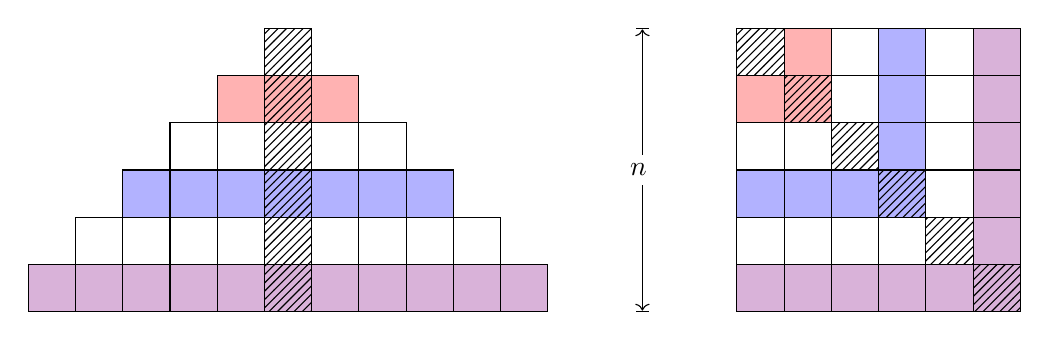
\begin{tikzpicture}[scale=0.6]
    \begin{scope}[shift={(0,0)}]
      \foreach \r/\f in{1/white,2/red!30,3/white,4/blue!30,5/white,6/violet!30}{
        \draw[fill=\f](-\r,-\r) rectangle(\r-1,1-\r);
        \draw(-\r,-\r)grid(\r-1,1-\r);
        \draw[pattern=north east lines, pattern color=black](-1,-\r) rectangle(0,1-\r);
      }    
    \end{scope}
    \begin{scope}[shift={(7,0)}]
      \draw[|<->|](0,0)--(0,-6) node[midway,fill=white]{$n$层};
    \end{scope}
    \begin{scope}[shift={(9,0)}]
      \foreach \r/\f in{1/white,2/red!30,3/white,4/blue!30,5/white,6/violet!30}{
        \draw[fill=\f](0,-\r) rectangle(\r,1-\r);
        \draw(0,-\r)grid(\r,1-\r);
        \draw[fill=\f](\r,0) rectangle(\r-1,-\r);
        \draw(\r,0) grid(\r-1,-\r);
        \draw[pattern=north east lines, pattern color=black](\r-1,1-\r) rectangle(\r,-\r);
      }
    \end{scope}
  \end{tikzpicture}
\end{center}

\begin{example}
  前$n$个数的和是$\dfrac{(n+1)}{2}$,即
  \begin{align}
    1+2+3+\cdots+n=\frac{n(n+1)}{2}
  \end{align}
\end{example}
\begin{center}
  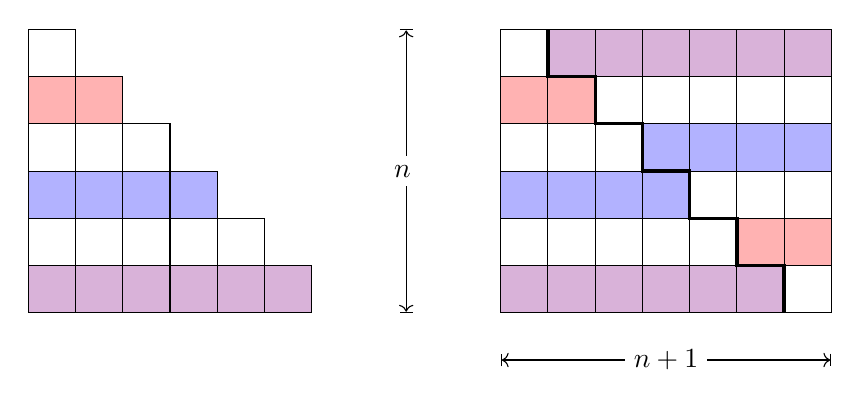
\begin{tikzpicture}[scale=0.6]
    \begin{scope}[shift={(0,0)}]
      \foreach \r/\f in{1/white,2/red!30,3/white,4/blue!30,5/white,6/violet!30}{
        \draw[fill=\f](0,1-\r) rectangle(\r, -\r);
        \draw(0,1-\r) grid(\r, -\r);
      }    
    \end{scope}
    \begin{scope}[shift={(8,0)}]
      \draw[|<->|](0,0)--(0,-6) node[midway,fill=white]{$n$层};
    \end{scope}
    \begin{scope}[shift={(10,0)}]
      \foreach \r/\f in{1/white,2/red!30,3/white,4/blue!30,5/white,6/violet!30}{
        \draw[fill=\f](0,1-\r) rectangle(\r, -\r);
        \draw(0,1-\r) grid(\r, -\r);
      }
      \foreach \r/\f in{1/violet!30,2/white,3/blue!30,4/white,5/red!30,6/white}{
        \draw[fill=\f](\r,1-\r) rectangle(7, -\r);
        \draw(\r,1-\r) grid(7, -\r);
      }
      \draw[very thick](1,0)--(1,-1)--(2,-1)--(2,-2)--(3,-2)--(3,-3)
                     --(4,-3)--(4,-4)--(5,-4)--(5,-5)--(6,-5)--(6,-6);
      \draw[|<->|](0,-7)--(7,-7) node[midway,fill=white]{$n+1$};      
    \end{scope}
  \end{tikzpicture}
\end{center}

\begin{example}
  \begin{align*}
    1+2+3+\cdots+(n-1)=\binom n2
  \end{align*}
  \begin{center}
    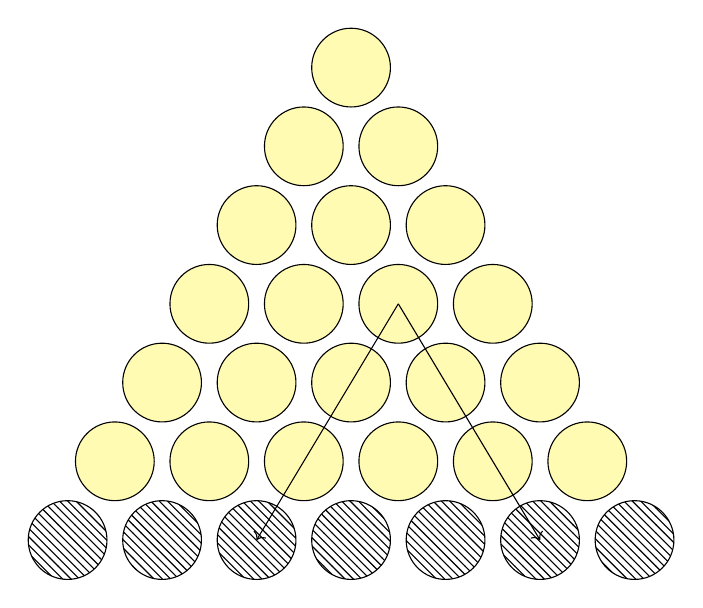
\begin{tikzpicture}[scale=1.0]
      \begin{scope}[shift={(0,0)}]
        \foreach \x/\y in {
          0/0,
          -.6/-1,.6/-1,
          -1.2/-2,0/-2,1.2/-2,
          -1.8/-3,-.6/-3,.6/-3,1.8/-3,
          -2.4/-4,-1.2/-4,0/-4,1.2/-4,2.4/-4,
          -3.0/-5,-1.8/-5,-.6/-5,.6/-5,1.8/-5,3.0/-5
          }{
            \draw[fill=yellow!30](\x,\y)circle(.5);
          }
          \foreach \x/\y in {
            -3.6/-6,-2.4/-6,-1.2/-6,0/-6,1.2/-6,2.4/-6,3.6/-6
          }{
            \draw[pattern=north west lines](\x,\y)circle(.5);
          }
          \draw[->](.6,-3)--(-1.2,-6);
          \draw[->](.6,-3)--(2.4,-6);
      \end{scope}
    \end{tikzpicture}
  \end{center}

  如图,在$7$个带阴影的圆中选$2$个,每种选法与其上某个圆圈一一对应,即三个圆圆心组成一个等腰三角形。
\end{example}

\pagebreak
\newcommand{\fixedcirclenode}[3]{\draw #1 circle(#2) node {#3};}
\begin{example}
  \begin{align*}
    1^2+2^2+3^2+\cdots=\frac{n(n+1)(2n+1)}6
  \end{align*}
  \centering
  \begin{tikzpicture}[scale=.6]
    \begin{scope}[shift={(0,0)}]
      \fixedcirclenode{(0,0)}{.5}{1};
      \fixedcirclenode{(-.5,-1)}{.5}{2}; \fixedcirclenode{(.5,-1)}{.5}{2};
      \fixedcirclenode{(-1,-2)}{.5}{3};  \fixedcirclenode{(0,-2)}{.5}{3};  \fixedcirclenode{(1,-2)}{.5}{3}; 
      \fixedcirclenode{(-1.5,-3)}{.5}{4};  \fixedcirclenode{(-.5,-3)}{.5}{4};  \fixedcirclenode{(.5,-3)}{.5}{4}; \fixedcirclenode{(1.5,-3)}{.5}{4}; \fixedcirclenode{(-2,-4)}{.5}{$\cdots$};
      \fixedcirclenode{(-1,-4)}{.5}{$\cdots$};  \fixedcirclenode{(0,-4)}{.5}{$\cdots$}; \fixedcirclenode{(1,-4)}{.5}{$\cdots$}; \fixedcirclenode{(2,-4)}{.5}{$\cdots$}; 
      \fixedcirclenode{(-2.5,-5)}{.5}{$n$}; \fixedcirclenode{(-1.5,-5)}{.5}{$n$};  \fixedcirclenode{(-.5,-5)}{.5}{$\cdots$};  \fixedcirclenode{(.5,-5)}{.5}{$\cdots$}; \fixedcirclenode{(1.5,-5)}{.5}{$n$}; \fixedcirclenode{(2.5,-5)}{.5}{$n$}; 
    \end{scope}
    
    \begin{scope}[shift={(3.5,0)}]
      \node at (0,-2) {{\huge $+$}};
    \end{scope}

    \begin{scope}[shift={(7,0)}]
      \fixedcirclenode{(0,0)}{.5}{$n$};
      \fixedcirclenode{(-.5,-1)}{.5}{$\cdots$}; \fixedcirclenode{(.5,-1)}{.5}{$n$};
      \fixedcirclenode{(-1,-2)}{.5}{4};  \fixedcirclenode{(0,-2)}{.5}{$\cdots$};  \fixedcirclenode{(1,-2)}{.5}{$\cdots$}; 
      \fixedcirclenode{(-1.5,-3)}{.5}{3}; \fixedcirclenode{(-.5,-3)}{.5}{4}; \fixedcirclenode{(.5,-3)}{.5}{$\cdots$}; \fixedcirclenode{(1.5,-3)}{.5}{$\cdots$}; 
      \fixedcirclenode{(-2,-4)}{.5}{2};  \fixedcirclenode{(-1,-4)}{.5}{3};  \fixedcirclenode{(0,-4)}{.5}{4}; \fixedcirclenode{(1,-4)}{.5}{$\cdots$}; \fixedcirclenode{(2,-4)}{.5}{$n$}; 
      \fixedcirclenode{(-2.5,-5)}{.5}{1}; \fixedcirclenode{(-1.5,-5)}{.5}{2};  \fixedcirclenode{(-.5,-5)}{.5}{3};  \fixedcirclenode{(.5,-5)}{.5}{4}; \fixedcirclenode{(1.5,-5)}{.5}{$\cdots$}; \fixedcirclenode{(2.5,-5)}{.5}{$n$}; 
    \end{scope}

    \begin{scope}[shift={(10.5,0)}]
      \node at (0,-2) {{\huge $+$}};
    \end{scope}
    
    \begin{scope}[shift={(14,0)}]
      \fixedcirclenode{(0,0)}{.5}{$n$};
      \fixedcirclenode{(-.5,-1)}{.5}{$n$}; \fixedcirclenode{(.5,-1)}{.5}{$\cdots$};
      \fixedcirclenode{(-1,-2)}{.5}{$\cdots$}; \fixedcirclenode{(0,-2)}{.5}{$\cdots$};  \fixedcirclenode{(1,-2)}{.5}{4}; 
      \fixedcirclenode{(-1.5,-3)}{.5}{$\cdots$};  \fixedcirclenode{(-.5,-3)}{.5}{$\cdots$};  \fixedcirclenode{(.5,-3)}{.5}{4}; \fixedcirclenode{(1.5,-3)}{.5}{3};
      \fixedcirclenode{(-2,-4)}{.5}{$n$};  \fixedcirclenode{(-1,-4)}{.5}{$\cdots$};  \fixedcirclenode{(0,-4)}{.5}{4}; \fixedcirclenode{(1,-4)}{.5}{3}; \fixedcirclenode{(2,-4)}{.5}{2}; 
      \fixedcirclenode{(-2.5,-5)}{.5}{$n$}; \fixedcirclenode{(-1.5,-5)}{.5}{$\cdots$};  \fixedcirclenode{(-.5,-5)}{.5}{4};  \fixedcirclenode{(.5,-5)}{.5}{3}; \fixedcirclenode{(1.5,-5)}{.5}{2}; \fixedcirclenode{(2.5,-5)}{.5}{1}; 
    \end{scope}
  \end{tikzpicture}

  \vspace*{2cm}
  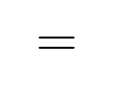
\begin{tikzpicture}[scale=1.4]
    \node at (-3,-2) {{\huge $=$}};
    \begin{scope}[shift={(0,0)}]
      \fixedcirclenode{(0,0)}{.5}{$2n+1$};
      \fixedcirclenode{(-.5,-1)}{.5}{$2n+1$}; \fixedcirclenode{(.5,-1)}{.5}{$2n+1$};
      \fixedcirclenode{(-1,-2)}{.5}{$2n+1$};  \fixedcirclenode{(0,-2)}{.5}{$2n+1$};  \fixedcirclenode{(1,-2)}{.5}{$2n+1$}; 
      \fixedcirclenode{(-1.5,-3)}{.5}{$2n+1$};  \fixedcirclenode{(-.5,-3)}{.5}{$2n+1$};  \fixedcirclenode{(.5,-3)}{.5}{$2n+1$}; \fixedcirclenode{(1.5,-3)}{.5}{$2n+1$}; \fixedcirclenode{(-2,-4)}{.5}{$\cdots$};
      \fixedcirclenode{(-1,-4)}{.5}{$\cdots$};  \fixedcirclenode{(0,-4)}{.5}{$\cdots$}; \fixedcirclenode{(1,-4)}{.5}{$\cdots$}; \fixedcirclenode{(2,-4)}{.5}{$\cdots$}; 
      \fixedcirclenode{(-2.5,-5)}{.5}{$2n+1$}; \fixedcirclenode{(-1.5,-5)}{.5}{$2n+1$};  \fixedcirclenode{(-.5,-5)}{.5}{$\cdots$};  \fixedcirclenode{(.5,-5)}{.5}{$\cdots$}; \fixedcirclenode{(1.5,-5)}{.5}{$2n+1$}; \fixedcirclenode{(2.5,-5)}{.5}{$2n+1$}; 
    \end{scope}
  \end{tikzpicture}
  \begin{align*}
    \text{从而有}\quad 3\left(1^2+2^2+3^2+\cdots+n^2\right) = (2n+1)\cdot \frac{n(n+1)}2
  \end{align*}
\end{example}

\pagebreak
\begin{example}[维维亚尼定理,Viviani's Theorem]
  记等边三角形的高为$h$,三角形内任意一点$P$到三边的距离分别为$l,m,n$,则
  \begin{align}
    h=l+m+n
  \end{align}
\end{example}
\begin{center}
  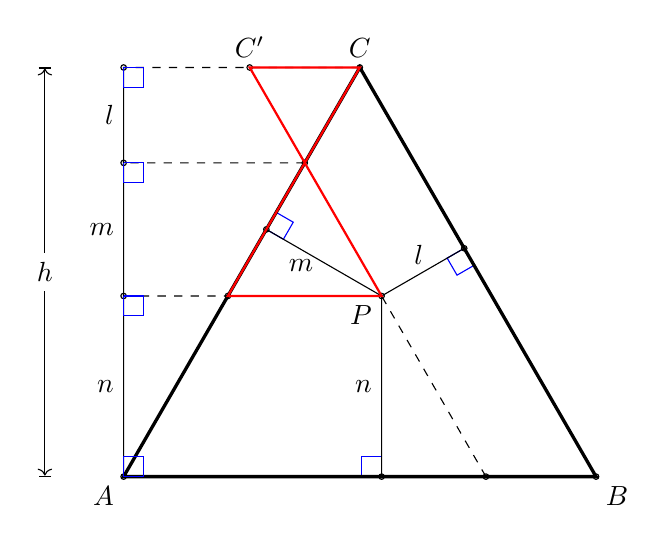
\begin{tikzpicture}[scale=1]
    \tkzDefPoint[label=below left:$A$](0,0){A}
    \tkzDefPoint[label=below right:$B$](6,0){B}
    \tkzDefPoint[label=above:$C$](60:6){C} %polar coordinate
    \tkzDefPoint[label=below left:$P$](35:4){P}
    \coordinate(D) at ($(B)!(P)!(C)$);
    \coordinate(E) at ($(C)!(P)!(A)$);
    \coordinate(F) at ($(A)!(P)!(B)$);

    \coordinate(Q) at (0,6);
    \coordinate(C'') at ($(A)!(C)!(Q)$);
    \coordinate(P'') at ($(A)!(P)!(Q)$);
    \coordinate(MN) at($(P) + (120:6)$);
    \tkzInterLL(P,MN)(A,C)\tkzGetPoint{M};
    \tkzInterLL(P,MN)(A,B)\tkzGetPoint{N};
    \tkzInterLL(P,MN)(C,C'')\tkzGetPoint{C'};
    \tkzInterLL(P,P'')(A,C)\tkzGetPoint{P'};
    
    \coordinate(M'') at($(A)!(M)!(Q)$);

    % the altitude
    \coordinate(H) at (-1,0);
    \coordinate(H') at (-1,6);
    \coordinate(H'') at ($(H)!(C)!(H')$);
    \draw[|<->|](H)--(H'') node[midway,fill=white]{$h$};

    \tkzMarkRightAngle[color=blue](B,D,P)
    \tkzMarkRightAngle[color=blue](C,E,P)
    \tkzMarkRightAngle[color=blue](A,F,P)

    \tkzDrawPoints(A,B,C,P,D,E,F,C',C'',P',P'',M,M'',N);
    \tkzLabelPoints[above](C')

    \draw[very thick](A)--(B)--(C)--cycle;
    \draw(P)--(D) node[pos=0.45,above]{$l$}
         (P)--(E) node[pos=0.7, below]{$m$}
         (P)--(F) node[midway, left]{$n$}
         (A)--(P'') node[midway, left]{$n$}
         (P'')--(M'') node[midway,left]{$m$}
         (M'')--(C'') node[midway,left]{$l$};
    \draw[dashed](P)--(P'') (M)--(M'') (C)--(C'') (N)--(C');
    \tkzMarkRightAngle[color=blue](P,P'',A)
    \tkzMarkRightAngle[color=blue](M,M'',A)
    \tkzMarkRightAngle[color=blue](C,C'',A)
    \tkzMarkRightAngle[color=blue](Q,A,B)

    \draw[red,thick](P)--(P')--(C)--(C')--cycle;
  \end{tikzpicture}
\end{center}

\begin{center}
  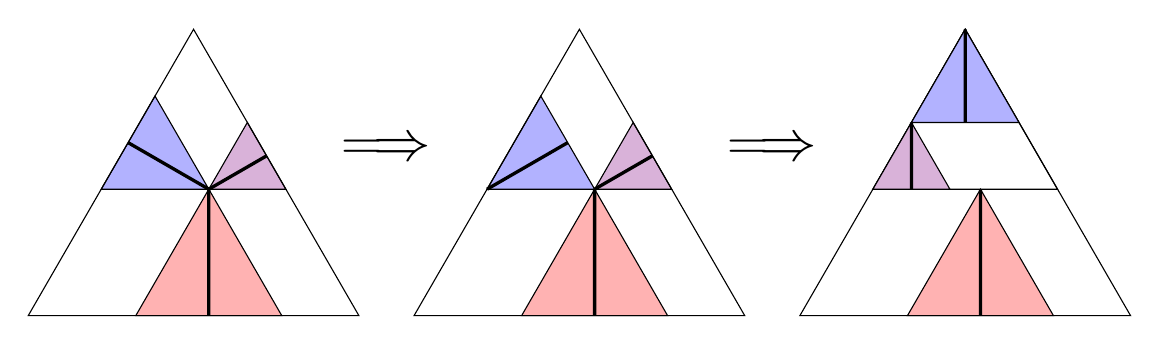
\begin{tikzpicture}[scale=.7]
    \begin{scope}[shift={(0,0)}]
      \tkzDefPoint(0,0){A}
      \tkzDefPoint(6,0){B}
      \tkzDefPoint(60:6){C} %polar coordinate
      \tkzDefPoint(35:4){P}
      \coordinate(D) at ($(B)!(P)!(C)$);
      \coordinate(E) at ($(C)!(P)!(A)$);
      \coordinate(F) at ($(A)!(P)!(B)$);
      
      \coordinate(F1) at ($(P)!sqrt(4/3)!30:(F)$);
      \coordinate(F2) at ($(P)!sqrt(4/3)!-30:(F)$);

      \coordinate(E1) at ($(P)!sqrt(4/3)!30:(E)$);
      \coordinate(E2) at ($(P)!sqrt(4/3)!-30:(E)$);

      \coordinate(D1) at ($(P)!sqrt(4/3)!30:(D)$);
      \coordinate(D2) at ($(P)!sqrt(4/3)!-30:(D)$);
      
      \coordinate(O) at ($1/3*(P)+1/3*(E1)+1/3*(E2)$);
      \calcLength(O,E1){r}
      \centerarc[->](O)(75:-15:\r pt);
      \centerarc[->](O)(-45:-135:\r pt);
      \centerarc[->](O)(-165:-255:\r pt);

      \draw[fill=red!30] (P)--(F1)--(F2)--cycle;
      \draw[fill=violet!30] (P)--(D1)--(D2)--cycle;
      \draw[fill=blue!30]  (P)--(E1)--(E2)--cycle;
      \draw (A)--(B)--(C)--cycle;
      \draw[very thick] (P)--(D) (P)--(E) (P)--(F);
    \end{scope}
    \begin{scope}[shift={(6.5,3)}]
      \node at (0,0) {\huge $\implies$};
    \end{scope}
    \begin{scope}[shift={(7,0)}]
      \tkzDefPoint(0,0){A}
      \tkzDefPoint(6,0){B}
      \tkzDefPoint(60:6){C} %polar coordinate
      \tkzDefPoint(35:4){P}
      \coordinate(D) at ($(B)!(P)!(C)$);
      \coordinate(E) at ($(C)!(P)!(A)$);
      \coordinate(F) at ($(A)!(P)!(B)$);
      
      \coordinate(F1) at ($(P)!sqrt(4/3)!30:(F)$);
      \coordinate(F2) at ($(P)!sqrt(4/3)!-30:(F)$);

      \coordinate(E1) at ($(P)!sqrt(4/3)!30:(E)$);
      \coordinate(E2) at ($(P)!sqrt(4/3)!-30:(E)$);

      \coordinate(D1) at ($(P)!sqrt(4/3)!30:(D)$);
      \coordinate(D2) at ($(P)!sqrt(4/3)!-30:(D)$);

      \coordinate(E') at ($(E2)!(E1)!(P)$);
      
      \draw[fill=red!30] (P)--(F1)--(F2)--cycle;
      \draw[fill=violet!30] (P)--(D1)--(D2)--cycle;
      \draw[fill=blue!30]  (P)--(E1)--(E2)--cycle;
      \draw (A)--(B)--(C)--cycle;
      \draw[very thick] (P)--(D) (E1)--(E') (P)--(F);

      \coordinate(O) at ($1/3*(C)+1/3*(E1)+1/3*(D2)$);
      \calcLength(O,E1){r}
      \centerarc[->](O)(75:-15:\r pt);
      \centerarc[->](O)(-45:-135:\r pt);
      \centerarc[->](O)(-165:-255:\r pt);
    \end{scope}
    \begin{scope}[shift={(13.5,3)}]
      \node at (0,0) {\huge $\implies$};
    \end{scope}
    \begin{scope}[shift={(14,0)}]
      \tkzDefPoint(0,0){A}
      \tkzDefPoint(6,0){B}
      \tkzDefPoint(60:6){C} %polar coordinate
      \tkzDefPoint(35:4){P}
      \coordinate(D) at ($(B)!(P)!(C)$);
      \coordinate(E) at ($(C)!(P)!(A)$);
      \coordinate(F) at ($(A)!(P)!(B)$);
      
      \coordinate(F1) at ($(P)!sqrt(4/3)!30:(F)$);
      \coordinate(F2) at ($(P)!sqrt(4/3)!-30:(F)$);

      \coordinate(E1) at ($(P)!sqrt(4/3)!30:(E)$);
      \coordinate(E2) at ($(P)!sqrt(4/3)!-30:(E)$);

      \coordinate(D1) at ($(P)!sqrt(4/3)!30:(D)$);
      \coordinate(D2) at ($(P)!sqrt(4/3)!-30:(D)$);

      \coordinate(E') at ($(E2)!(E1)!(P)$);
      
      \draw[fill=red!30] (P)--(F1)--(F2)--cycle;
      \draw (A)--(B)--(C)--cycle;
      \draw[very thick] (P)--(F);
      \draw (C)--(E1)--(D2)--cycle;

      \coordinate(O) at ($1/3*(C)+1/3*(E1)+1/3*(D2)$);
      \coordinate(P) at ($(O)!1!-120:(P)$);
      \coordinate(D1) at ($(O)!1!-120:(D1)$);
      \coordinate(D2) at ($(O)!1!-120:(D2)$);
      \coordinate(D)  at ($(O)!1!-120:(D)$);
      \coordinate(E1) at ($(O)!1!-120:(E1)$);
      \coordinate(E2) at ($(O)!1!-120:(E2)$);
      \coordinate(E') at ($(O)!1!-120:(E')$);
      % \draw(C)--(O);
      % \begin{scope}[rotate around={-60:(O)}]
        \draw[rotate around={-120:(O)},fill=violet!30] (P)--(D1)--(D2)--cycle;
        \draw[rotate around={-120:(O)},fill=blue!30] (P)--(E1)--(E2)--cycle;
        \draw[rotate around={-120:(O)},very thick] (P)--(D) (E1)--(E');
      % \end{scope}
    \end{scope}
  \end{tikzpicture}
\end{center}

\pagebreak
\begin{example}%\mbox{}\par\nopagebreak
  \begin{align*}
    \sum\limits_{n=1}^\infty \left(\dfrac14\right)^n = \dfrac13
  \end{align*}
\centering
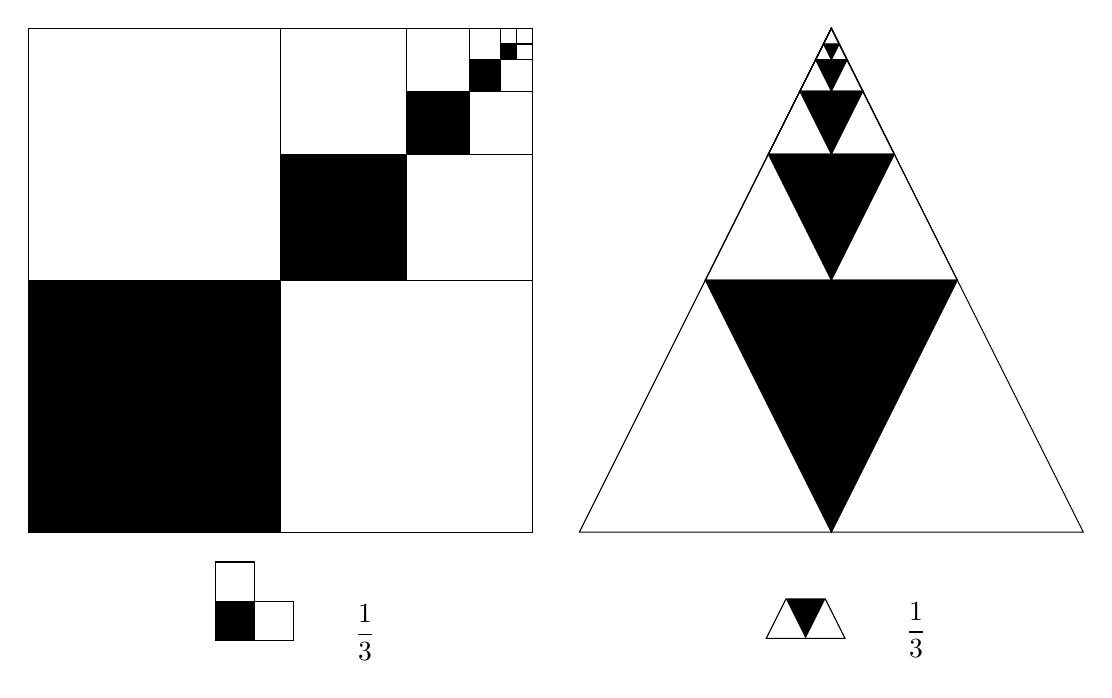
\begin{tikzpicture}[scale=0.2]
  \begin{scope}[shift={(0,0)}]
    % \node[left] at (-40,-16) {$\sum\limits_{n=1}^\infty \left(\dfrac14\right)^n = \dfrac13$};
    \draw(0,-1)rectangle(-1,0) rectangle(-2,-1)rectangle(-1,-2)rectangle(0,-1);
    \fill(-1,-1)rectangle(-2,-2);

    \draw[scale=2](0,-1)rectangle(-1,0) rectangle(-2,-1)rectangle(-1,-2)rectangle(0,-1);
    \fill[scale=2](-1,-1)rectangle(-2,-2);

    \draw[scale=4](0,-1)rectangle(-1,0) rectangle(-2,-1)rectangle(-1,-2)rectangle(0,-1);
    \fill[scale=4](-1,-1)rectangle(-2,-2);

    \draw[scale=8](0,-1)rectangle(-1,0) rectangle(-2,-1)rectangle(-1,-2)rectangle(0,-1);
    \fill[scale=8](-1,-1)rectangle(-2,-2);

    \draw[scale=16](0,-1)rectangle(-1,0)rectangle(-2,-1)rectangle(-1,-2)rectangle(0,-1);
    \fill[scale=16](-1,-1)rectangle(-2,-2);

    \node at(-16,-37) {每个\hskip5pt\tikz[scale=0.5]{\fill(0,0)rectangle(1,1);\draw(0,1)rectangle(1,2) (1,0)rectangle(2,1);}\hskip5pt 中阴影部分占$\dfrac13$};
  \end{scope}

  \begin{scope}[shift={(19,0)}]
    \draw(0,0)--(-1,-2)--(1,-2)--cycle;
    \fill[draw](-.5,-1)--(0,-2)--(.5,-1)--cycle;

    \draw[scale=2](0,0)--(-1,-2)--(1,-2)--cycle;
    \fill[scale=2,draw](-.5,-1)--(0,-2)--(.5,-1)--cycle;

    \draw[scale=4](0,0)--(-1,-2)--(1,-2)--cycle;
    \fill[scale=4,draw](-.5,-1)--(0,-2)--(.5,-1)--cycle;

    \draw[scale=8](0,0)--(-1,-2)--(1,-2)--cycle;
    \fill[scale=8,draw](-.5,-1)--(0,-2)--(.5,-1)--cycle;

    \draw[scale=16](0,0)--(-1,-2)--(1,-2)--cycle;
    \fill[scale=16,draw](-.5,-1)--(0,-2)--(.5,-1)--cycle;

    \node at(0,-38.1) {每个\hskip5pt\tikz[scale=0.5]{\fill(-.5,-1)--(0,-2)--(.5,-1)--cycle;\draw(-.5,-1)--(-1,-2)--(1,-2)--(.5,-1)--cycle;}\hskip5pt 中阴影部分占$\dfrac13$};
  \end{scope}
\end{tikzpicture}


\end{example}

\begin{example}
  证明:$3<\pi<4$。

\begin{center}
  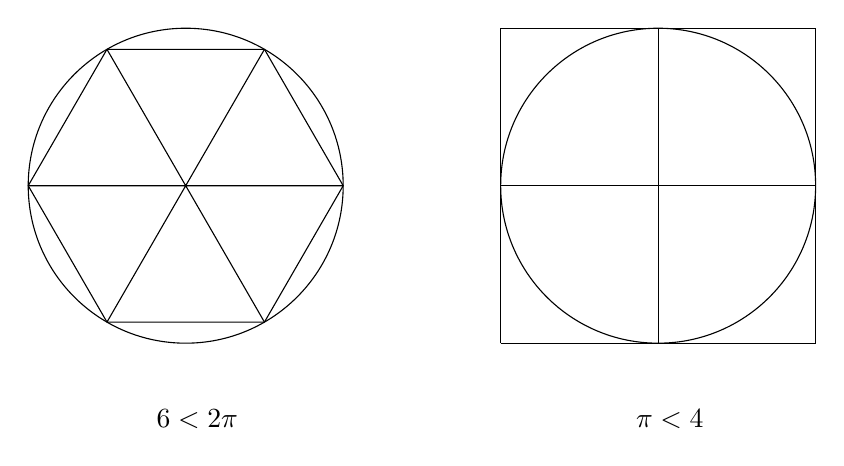
\begin{tikzpicture}[scale=2]
    \begin{scope}[shift={(0,0)}]
      \draw(0,0)circle(1);
      \draw(0:1)\foreach \x in {60,120,...,360} {  -- (\x:1) } --cycle;
      \draw(0:1)--(180:1) (60:1)--(240:1) (120:1)--(300:1);
      \node[label=below:{比周长$6<2\pi$}] at (0,-1.3) {};
    \end{scope}
    \begin{scope}[shift={(3,0)}]
      \draw(0,0)circle(1);
      \draw(-1,-1)grid(1,1);
      \node[label=below:{比面积$\pi<4$}] at (0,-1.3) {};
    \end{scope}
  \end{tikzpicture}
\end{center}
\end{example}


\pagebreak
\begin{example}
  正方形$ABCD$和直角三角形$ABE$,则$\angle AEB$的角平分线将正方形$ABCE$分为两个全等的部分。\nopagebreak

  % \nopagebreak has no effect before a \begin{center} environment
\centering
  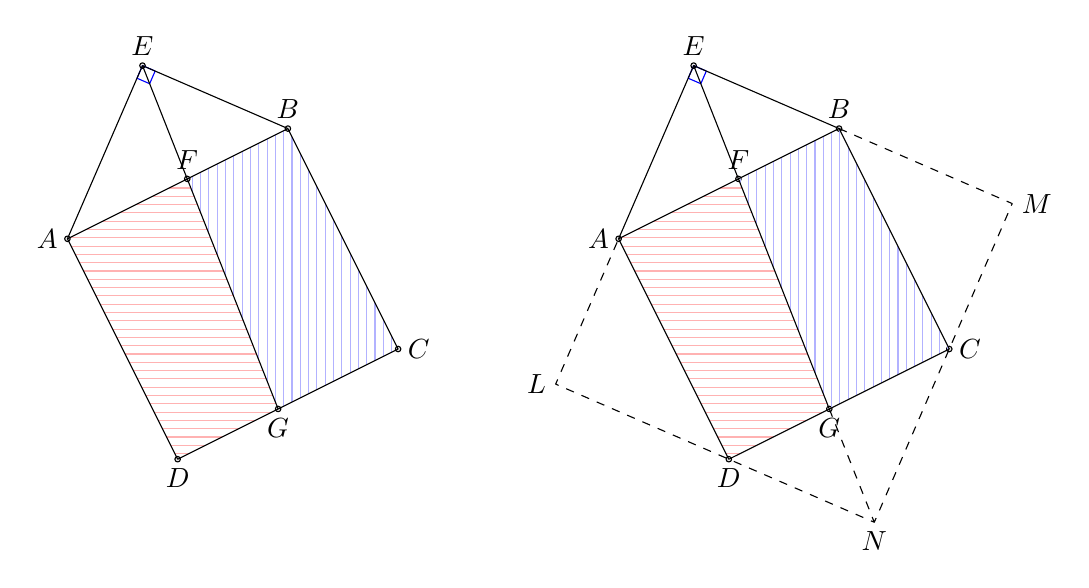
\begin{tikzpicture}[scale=.7,line join=round]
    \begin{scope}[shift={(0,0)}]
      \coordinate[label=left:$A$](A) at (0,0);
      \coordinate[label=above:$B$](B) at (4,2);
      \coordinate[label=right:$C$](C) at ($(B)!1!90:(A)$);
      \coordinate[label=below:$D$](D) at ($(C)!1!90:(B)$);
      \coordinate(E') at ($(B)!0.2!-50:(A)$);
      \coordinate[label=above:$E$](E) at ($(B)!(A)!(E')$);

      % middle of AB
      % \coordinate[label=above right:$F$](F) at ($(A)!.5!(B)$);
      % bisector of AEB
      \tkzDefLine[bisector](A,E,B)\tkzGetPoint{f}
      \tkzInterLL(A,B)(E,f)\tkzGetPoint{F}\tkzLabelPoints[above](F)

      \tkzInterLL(E,F)(C,D)\tkzGetPoint{G}\tkzLabelPoints[below](G)
      \tkzDrawPoints(A,B,C,D,E,F,G)

      \tkzMarkRightAngle[color=blue](B,E,A);
      \fill[pattern=horizontal lines,pattern color=red!30](A)--(F)--(G)--(D)--cycle;
      \fill[pattern=vertical lines,pattern color=blue!30](F)--(G)--(C)--(B)--cycle;
      \draw(A)--(B)--(C)--(D)--cycle;
      \draw(A)--(E)--(B) (E)--(F)--(G);
    \end{scope}

    \begin{scope}[shift={(10,0)}]
      \coordinate[label=left:$A$](A) at (0,0);
      \coordinate[label=above:$B$](B) at (4,2);
      \coordinate[label=right:$C$](C) at ($(B)!1!90:(A)$);
      \coordinate[label=below:$D$](D) at ($(C)!1!90:(B)$);
      \coordinate(E') at ($(B)!0.2!-50:(A)$);
      \coordinate[label=above:$E$](E) at ($(B)!(A)!(E')$);

      % middle of AB
      % \coordinate[label=above right:$F$](F) at ($(A)!.5!(B)$);
      % bisector of AEB
      \tkzDefLine[bisector](A,E,B)\tkzGetPoint{f}
      \tkzInterLL(A,B)(E,f)\tkzGetPoint{F}\tkzLabelPoints[above](F)

      \tkzInterLL(E,F)(C,D)\tkzGetPoint{G}\tkzLabelPoints[below](G)
      \tkzDrawPoints(A,B,C,D,E,F,G)

      \tkzMarkRightAngle[color=blue](B,E,A);
      \fill[pattern=horizontal lines,pattern color=red!30](A)--(F)--(G)--(D)--cycle;
      \fill[pattern=vertical lines,pattern color=blue!30](F)--(G)--(C)--(B)--cycle;
      \draw(A)--(B)--(C)--(D)--cycle;
      \draw(A)--(E)--(B) (E)--(F)--(G);

      \coordinate[label=left:$L$](L) at ($(E)!(D)!(A)$);
      \coordinate[label=right:$M$](M) at ($(E)!(C)!(B)$);
      \tkzInterLL(M,C)(L,D)\tkzGetPoint{N}\tkzLabelPoints[below](N)
      \draw[dashed](B)--(M)--(C)--(N)--(D)--(L)--(A) (G)--(N);
    \end{scope}
  \end{tikzpicture}
\end{example}

\pagebreak
\begin{example}
  将$x^2+ax$配方,有
  \begin{align*}
    x^2+ax=\left(x+\frac a2\right)^2-\left(\frac a2\right)^2
  \end{align*}
\end{example}\nopagebreak
\begin{center}
  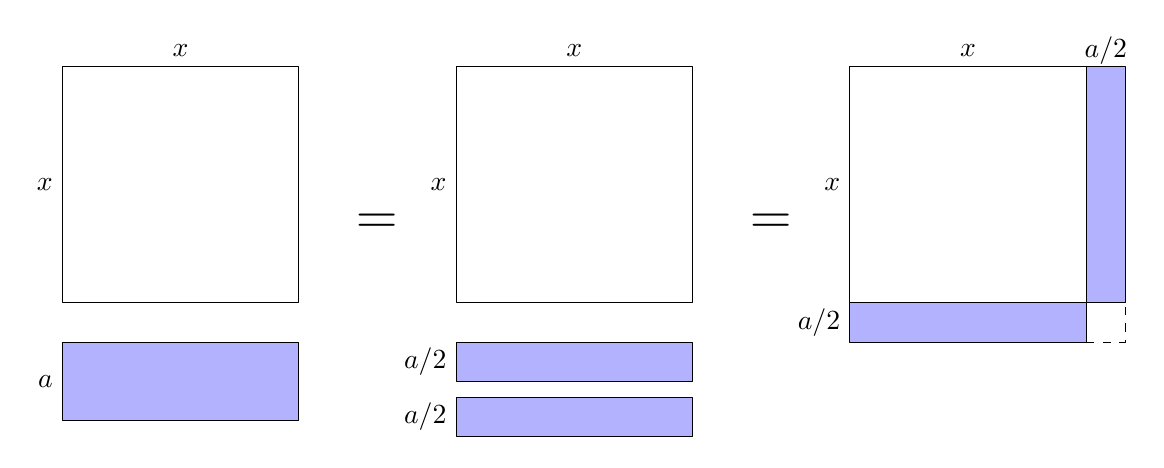
\begin{tikzpicture}[scale=1,line join=round]
    \begin{scope}[shift={(0,0)}]
      \draw (0,0)rectangle(3,3);
      \draw[fill=blue!30] (0,-.5) rectangle(3,-1.5);
      \node at (0,1.5)[left]{$x$};
      \node at (1.5,3)[above]{$x$};
      \node at (0,-1)[left]{$a$};
    \end{scope}
    
    \begin{scope}[shift={(4,0)}]
      \node at (0,1) {\huge $=$};
    \end{scope}
    
    \begin{scope}[shift={(5,0)}]
      \draw (0,0)rectangle(3,3);
      \draw[fill=blue!30] (0,-.5) rectangle(3,-1);
      \draw[fill=blue!30] (0,-1.2) rectangle(3,-1.7);
      \node at (0,1.5)[left]{$x$};
      \node at (1.5,3)[above]{$x$};
      \node at (0,-.75)[left]{$a/2$};
      \node at (0,-1.45)[left]{$a/2$};
    \end{scope}

    \begin{scope}[shift={(9,0)}]
      \node at (0,1) {\huge $=$};
    \end{scope}

    \begin{scope}[shift={(10,0)}]
      \draw (0,0)rectangle(3,3);
      \draw[fill=blue!30] (0,0) rectangle(3,-.5);
      \draw[fill=blue!30] (3,0) rectangle(3.5,3);
      \draw[dashed](3,-.5)--(3.5,-.5)--(3.5,0);
      \node at (0,1.5)[left]{$x$};
      \node at (1.5,3)[above]{$x$};
      \node at (0,-.25)[left]{$a/2$};
      \node at (3.25,2.9)[above]{$a/2$};
    \end{scope}
  \end{tikzpicture}
\end{center}

\begin{example}
  \begin{align*}
    (a+b)^2+(a-b)^2=2(a^2+b^2)
  \end{align*}
  \centering
  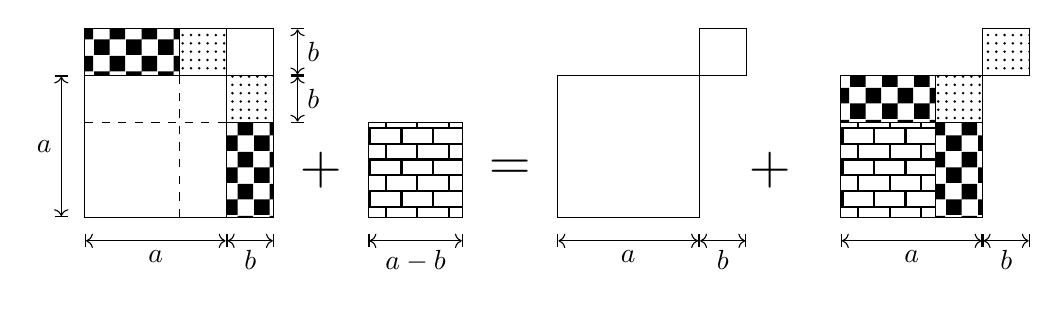
\begin{tikzpicture}[scale=.30]
    \begin{scope}[shift={(0,0)}]
      \draw(0,0)rectangle(8,8);
      \draw[pattern=checkerboard](6,0)rectangle(8,4) (0,6)rectangle(4,8);
      \draw[pattern=dots](6,4)rectangle(8,6) (4,6)rectangle(6,8);
      \draw[dashed](0,4)--(8,4) (4,0)--(4,8);
      \draw[|<->|](0,-1)--(6,-1)node[midway,below]{$a$};
      \draw[|<->|](6,-1)--(8,-1)node[midway,below]{$b$};
      \draw[|<->|](9,6)--(9,8)node[midway,right]{$b$};
      \draw[|<->|](9,6)--(9,4)node[midway,right]{$b$};
      \draw[|<->|](-1,0)--(-1,6)node[midway,left]{$a$};
    \end{scope}
    \node at(10,2) {\huge$+$};
    \begin{scope}[shift={(12,0)}]
      \draw[pattern=bricks](0,0)rectangle(4,4);
      \draw[|<->|](0,-1)--(4,-1)node[midway,,below]{$a-b$};
    \end{scope}
    \node at(18,2) {\huge$=$};
    \begin{scope}[shift={(20,0)}]
      \draw(0,0)rectangle(6,6)rectangle(8,8);
      \draw[|<->|](0,-1)--(6,-1)node[midway,,below]{$a$};
      \draw[|<->|](6,-1)--(8,-1)node[midway,,below]{$b$};
    \end{scope}
    \node at(29,2) {\huge$+$};
    \begin{scope}[shift={(32,0)}]
      \draw[pattern=bricks](0,0)rectangle(4,4);
      \draw[pattern=checkerboard](4,0)rectangle(6,4) (0,4)rectangle(4,6);
      \draw[pattern=dots](4,4)rectangle(6,6) rectangle(8,8);
      \draw[dashed](4,6)--(4,4)--(6,4);
      \draw[|<->|](0,-1)--(6,-1)node[midway,,below]{$a$};
      \draw[|<->|](6,-1)--(8,-1)node[midway,below]{$b$};
    \end{scope}
  \end{tikzpicture}
\end{example}

\pagebreak
\begin{example}[半角正切公式]\mbox{}\par\nopagebreak %to mandatorily make it break line
  \centering
    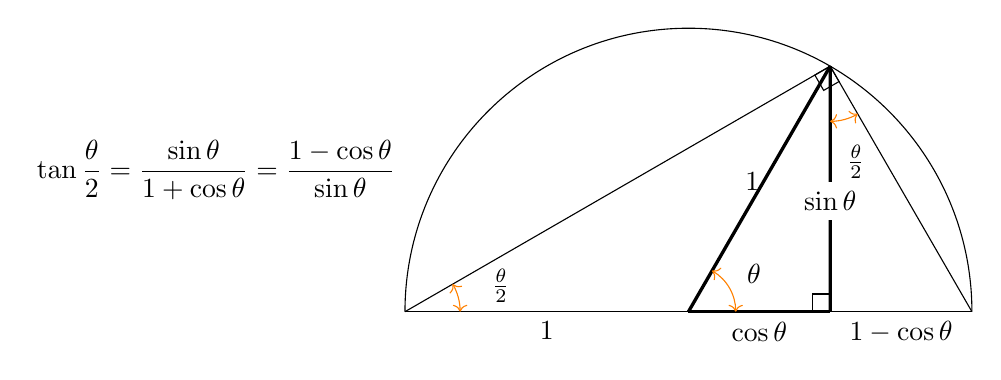
\begin{tikzpicture}[scale=.9]
      \coordinate (A) at (-4,0);
      \coordinate (O) at (0,0);
      \coordinate (B) at (4,0);
      \coordinate (C) at ($4*(.5, {sqrt(3)*.5})$);
      \coordinate (D) at ($(A)!(C)!(B)$);
      \tkzMarkRightAngle(B,C,A)\tkzMarkRightAngle(C,D,A)
      \draw(O)--(A) node[midway,below]{1};
      \draw[very thick](O)--(C) node[pos=.45,above]{1};
      \draw[very thick](C)--(D) node[pos=.55,fill=white]{$\sin\theta$};
      \draw[very thick](O)--(D) node[midway,below]{$\cos\theta$};
      \draw(D)--(B) node[midway,below]{$1-\cos\theta$};
      \draw(A)--(C)--(B);
      \draw(B)arc(0:180:4);
      \draw pic["$\theta$",<->,draw=orange,angle eccentricity=1.6,angle radius=.6cm]{angle=D--O--C};
      \draw pic["$\frac\theta2$",<->,draw=orange,angle eccentricity=1.8,angle radius=.7cm]{angle=O--A--C};
      \draw pic["$\frac\theta2$",<->,draw=orange,angle eccentricity=1.8,angle radius=.7cm]{angle=D--C--B};
      % \draw (C)--(A)--(B)--cycle--(D);
      \node[left] at (-4,2){$\tan\dfrac\theta2=\dfrac{\sin\theta}{1+\cos\theta}=\dfrac{1-\cos\theta}{\sin\theta}$};
    \end{tikzpicture}
\end{example}

\pagebreak
\begin{example}[反正切求和]\mbox{}\par\nopagebreak
\centering
  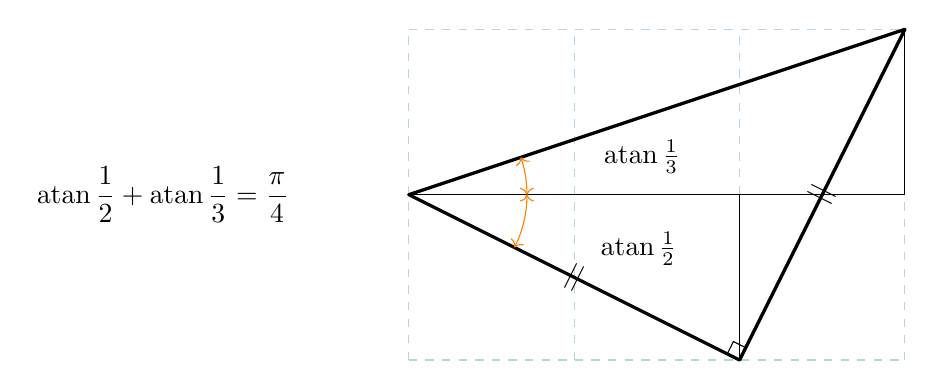
\begin{tikzpicture}[scale=0.7]
    \node[left] at (-2,3) {$\atan\dfrac12+\atan\dfrac13=\dfrac\pi4$};
    \coordinate (A) at (0,3);
    \coordinate (B) at (6,0);
    \coordinate (C) at (9,6);
    \coordinate (D) at (6,3);
    \coordinate (E) at (9,3);
    \draw[help lines,dashed](0,0)grid[step=3](9,6);
    \draw[very thick, line join=round](A)--(B)node[midway,sloped]{||}--(C)node[midway,sloped]{||}--cycle;
    \draw(A)--(E)--(C) (D)--(B);
    \draw pic["$\atan\frac12$",<->,draw=orange,angle eccentricity=2,angle radius=1.5cm]{angle=B--A--D};
    \draw pic["$\atan\frac13$",<->,draw=orange,angle eccentricity=2,angle radius=1.5cm]{angle=D--A--C};
    \tkzMarkRightAngle(A,B,C);
  \end{tikzpicture}

  \vspace*{2cm}

  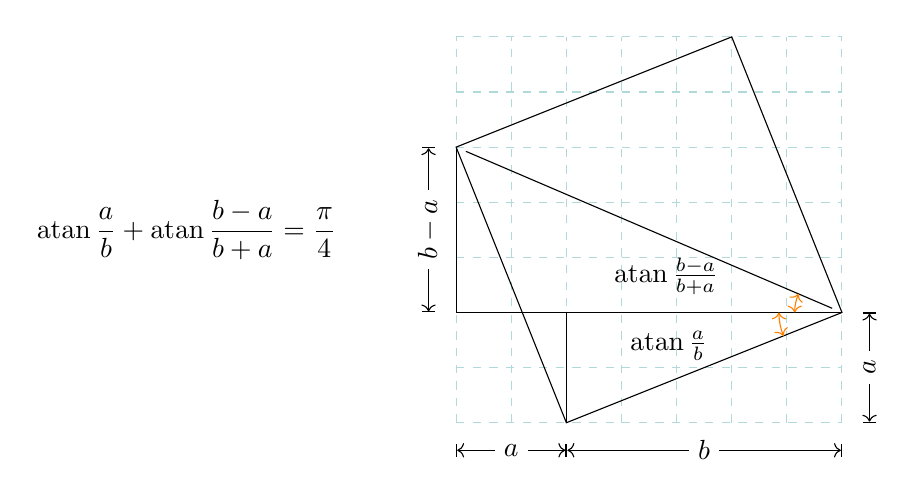
\begin{tikzpicture}[scale=0.7]
    \node[left] at (-2,3.5) {$\atan\dfrac ab+\atan\dfrac{b-a}{b+a}=\dfrac\pi4$};
    \draw[help lines,dashed](0,0)grid(7,7);
    \draw (2,0) node (A){} --(7,2) node (B){} --(5,7) node (C){} --(0,5)node (D){}--cycle;
    \draw (B)--(D);
    \draw (0,5)--(0,2)--(7,2) (2,2) node (E){} --(2,0);
    \draw pic["$\atan\frac ab$",<->,draw=orange,angle eccentricity=2.8,angle radius=.8cm]{angle=E--B--A};
    \draw pic["$\atan\frac {b-a}{b+a}$",<->,draw=orange,angle eccentricity=3.8,angle radius=.6cm]{angle=D--B--E};
    \draw[|<->|] (0,-.5)--(2,-.5)node[midway,fill=white]{$a$};
    \draw[|<->|] (2,-.5)--(7,-.5)node[midway,fill=white]{$b$};
    \draw[|<->|] (7.5,0)--(7.5,2)node[midway,fill=white,sloped]{$a$};
    \draw[|<->|] (-.5,2)--(-.5,5)node[midway,fill=white,sloped]{$b-a$};
  \end{tikzpicture}

  \vspace*{2cm}

  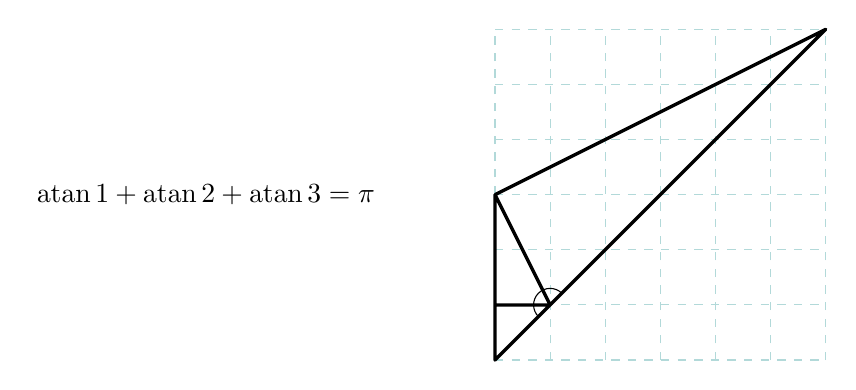
\begin{tikzpicture}[scale=0.7]
    \node[left] at(-2,3) {$\atan1+\atan2+\atan3=\pi$};
    \draw[help lines,dashed](0,0)grid(6,6);
    \draw[very thick, line join=round](0,1)--(1,1)--(0,0)--(0,3)--(1,1)--(6,6)--(0,3);
    % use coordinate transform to draw the arc: ([shift=(t:r)] x, y),
    % where (x,y) is the center and (t:r) is the polar coordinate of
    % starting point.
    \draw([shift=(225:0.3)] 1,1) arc(225:45:0.3);
  \end{tikzpicture}
\end{example}



\chapter{洞察}
\label{chap:insight}

{\bfseries\large 这里的内容,很多都是错误有误导的,如果你是容易被人误导的人,那么建议你不要继续看本节的内容,不要看,不要看,千万不要看。}\clearpage\pagebreak

\section{错误的证明}
\label{sec:wrong-proof}


\begin{example}[消失的方块]证明:$31.5=32.5$。

  \centering
  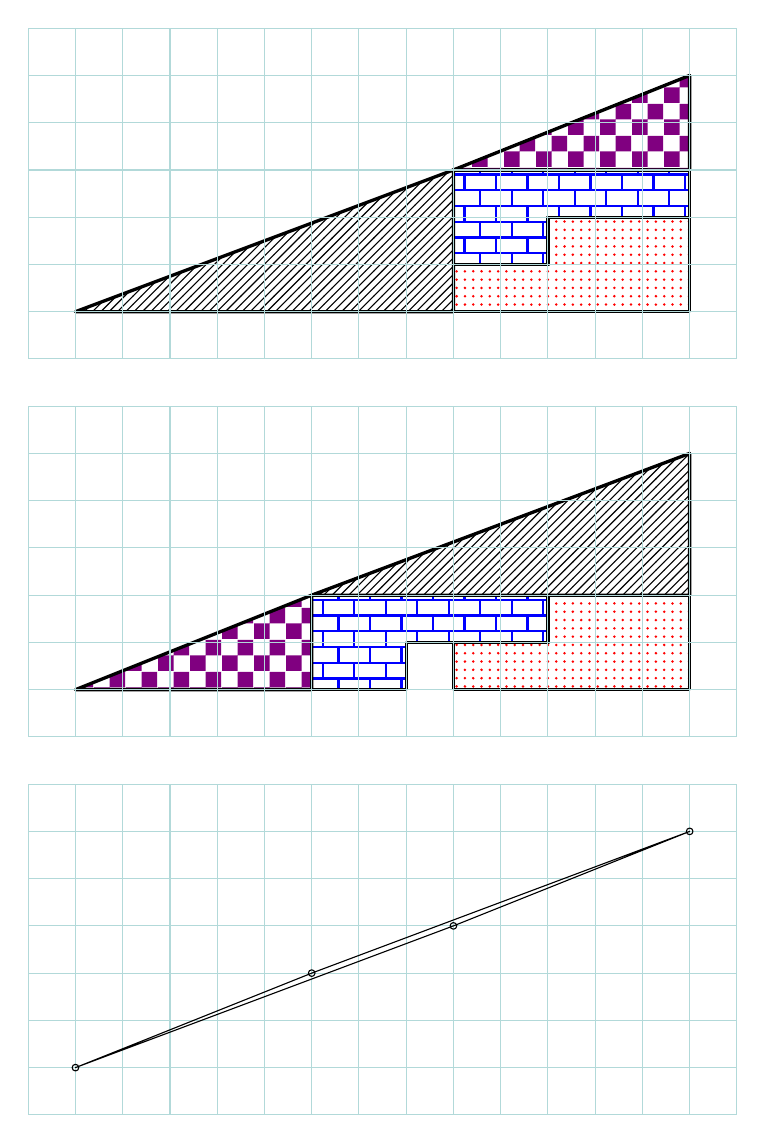
\begin{tikzpicture}[scale=0.6,line join=round]
    \begin{scope}[shift={(0,0)}]
      \draw[very thick,pattern=north east lines, pattern color=black](1,1)--(9,1)--(9,4)--cycle;
      \draw[very thick,pattern=dots, pattern color=red](9,1)--(14,1)--(14,3)--(11,3)--(11,2)--(9,2)--cycle;
      \draw[very thick,pattern=bricks, pattern color=blue](14,3)--(11,3)--(11,2)--(9,2)--(9,4)--(14,4)--cycle;
      \draw[very thick,pattern=checkerboard, pattern color=violet](9,4)--(14,4)--(14,6)--cycle;
      % \draw[very thick](1,1)--(14,1)--(14,6)--(9,4)--cycle;
      \draw[help lines](0,0)grid(15,7);
    \end{scope}
    \begin{scope}[shift={(0,-8)}]
      \draw[very thick,xshift=5cm,yshift=2cm,pattern=north east lines, pattern color=black](1,1)--(9,1)--(9,4)--cycle;
      \draw[very thick,pattern=dots, pattern color=red](9,1)--(14,1)--(14,3)--(11,3)--(11,2)--(9,2)--cycle;
      \draw[very thick,xshift=-3cm,yshift=-1cm,pattern=bricks, pattern color=blue](14,3)--(11,3)--(11,2)--(9,2)--(9,4)--(14,4)--cycle;
      \draw[very thick,xshift=-8cm,yshift=-3cm,pattern=checkerboard, pattern color=violet](9,4)--(14,4)--(14,6)--cycle;
      \draw[help lines](0,0)grid(15,7);
      % \draw[very thick](1,1)--(14,1)--(14,6)--(6,3)--cycle;
    \end{scope}
    \begin{scope}[shift={(0,-16)}]
      % \draw[very thick,xshift=5cm,yshift=2cm,pattern=north east lines, pattern color=black](1,1)--(9,1)--(9,4)--cycle;
      % \draw[very thick,pattern=dots, pattern color=red](9,1)--(14,1)--(14,3)--(11,3)--(11,2)--(9,2)--cycle;
      % \draw[very thick,xshift=-3cm,yshift=-1cm,pattern=bricks, pattern color=blue](14,3)--(11,3)--(11,2)--(9,2)--(9,4)--(14,4)--cycle;
      % \draw[very thick,xshift=-8cm,yshift=-3cm,pattern=checkerboard, pattern color=violet](9,4)--(14,4)--(14,6)--cycle;
      \draw[help lines](0,0)grid(15,7);
      \draw(1,1)--(6,3)--(14,6)--(9,4)--cycle;
      %\draw(1,1)--(14,6);
      %\draw[very thick](1,1)--(14,1)--(14,6)--(6,3)--cycle;
      \foreach \x/\y in {1/1,6/3,9/4,14/6}{%
        \draw(\x,\y)circle(2pt);
      }
    \end{scope}
  \end{tikzpicture}
\end{example}

\begin{proof}
  考虑阴影部分总面积,由上图,其面积为$\dfrac12\times13\times5=32.5$;由下图,其面积为$32.5-1=31.5$。而上下两图都是由相同组件组成,其面积应相同,从而有$32.5=31.5$。

  然而结论显然是错误的,也就是证明也是错误的。注意最后一图中四个点并不在一条直线上,所以根本原因在于最大的“三角形”并不是真正的三角形。差出来的一个格子的面积,就是图中四个点组成的四边形的面积\footnote{如果看不清的话,在电子文档上放大看。}。
\end{proof}


\fbox{\bfseries\noindent
  \begin{minipage}{.9\linewidth}
    注意!以下大多数的的求和“方法”在通常定义下都是错误的,请注意分辩。
  \end{minipage}
}

\begin{definition}[交错级数,Alternating Series]
  若$a_n\ge 0$,则$\sum(-1)^n a_n$称为交错级数,即正负相间的级数。
\end{definition}

\begin{theorem}[莱布尼茨定理]
  若交错级数中各项非负数列单调且趋于0,则级数收敛。即$\forall n$,$a_n\ge0$且$a_n\ge a_{n+1}$,则$\sum (-1)^n a_n$收敛,且其和$s\le a_1$(设$a_1$是第一个非0项),其余项$r_n$满足$|r_n|\le a_{n+1}$。
\end{theorem}
\begin{proof}[提示]
  $S_{n+1}-S_n=(-1)^{n+1} a_{n+1}$,从而$|S_n| - a_{n+1} \le |S_{n+1}|\le |S_n| + a_{n+1}$。
\end{proof}

\begin{definition}[阿贝尔和]
  $A(s)\equiv\lim\limits_{z\to1^{-}}\sum\limits_{n=1}^\infty a_nz^n$称为数列$s=\{a_1,a_2,\cdots\}$的阿贝尔和。
\end{definition}
\begin{example}[交错级数,Alternating Series]
  $1-2+3-4+5-6+\cdots$的阿贝尔和为$\frac14$。

  欧拉也曾研究过这个级数,他的设想与阿贝尔求和相似,他应用了如下的等式:
  \begin{align*}
    \frac1{(1+x)^2} = 1 - 2x + 3x^2 - 4x^3 + \cdots 
  \end{align*}
  至少这个等式在$|x|<1$时是成立,有很多种证明方法,比如泰勒展开,比如多项式长除。从而令$x$从左侧趋向于1,则可得级数的阿贝尔和为$\lim\limits_{x\to1^-}\dfrac{1}{(1+x)^2}=\frac14$。

  %\fbox{\noindent\begin{minipage}{.9\textwidth}
      也可以用一种直观的移位方式求出此交错级数的和。令
      \begin{align*}
        S_0 = 1 - 2 + 3 - 4 + \cdots
      \end{align*}
      将4个$S_0$相加,移位,上下对应位置数字相加,可得
      \begin{align*}\setlength\arraycolsep{2pt}
        \begin{array}{rccccccccccccc}
          4S_0 = &   &  &  &  &  &1 & -&2 & +&3 & -&4 & \cdots\\
                 & + &  &  &1  & -&2 & +&3 & -&4 & +&5 & \cdots\\
                 & + &  &  &1  & -&2 & +&3 & -&4 & +&5 & \cdots\\
                 & + &1 & -&2 & +&3 & -&4 & +&5 & -&6 & \cdots\\
               = &   &1 & +&0 & +&0 & +&0 & +&0 & +&0 & \cdots\\
               = &   &1
        \end{array}
      \end{align*}
      从而有$S_0=\frac14$。按这种方式,也可以得到$1-1+1-1+1-1+\cdots=\frac12$。问题出在哪里呢?如果序列是有限的,方法也许是可行的,然而对于无限的序列,特别是和是发散的无限级数,其和的定义都是不明确的,得出的结论自然也就与常识不符合。
    %\end{minipage}
  %}
\end{example}


\begin{example}
  所有正整数的和是$-\frac1{12}$。

  虽然这是个明显错误的结论,但下面的“证明”却“表明”了它是正确的,你能想明白为什么吗?

  \fbox{\small\begin{minipage}{.9\textwidth}
    令
    \begin{align*}
      S\phantom{_0}   =1+2+3+4+5+6+\cdots\\
      S_0 =1-2+3-4+5-6+\cdots
    \end{align*}
    那么
    \begin{align*}
      S - S_0 = 0 + 4 + 0 + 8 + 0 + 12 + 0 + \cdots = 4S
    \end{align*}
    从而$3S=-S_0$,由上面的交错级数和例子,有$S=-\frac1{12}$。
  \end{minipage}}
\end{example}

\section{数数}
\label{sec:count}


\begin{example}数一数,下面的图中有多少个三角形?
  \begin{center}
    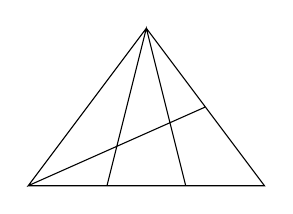
\begin{tikzpicture}[scale=1.0]
      \coordinate(A) at (0,0);
      \coordinate(B) at (1,0);
      \coordinate(C) at (2,0);
      \coordinate(D) at (3,0);
      \coordinate(F) at (1.5,2);
      \coordinate(E) at ($.5*(D)+.5*(F)$);
      \coordinate(G) at ($.75*(B)+.25*(F)$);
      \coordinate(H) at ($.6*(C)+.4*(F)$);
      \draw(A)--(D)--(F)--(A)--(G)--(H)--(E) (B)--(F)--(C);
    \end{tikzpicture}
  \end{center}
\end{example}
\begin{proof}[提示]
  单个格子组成的三角形:
  \begin{center}
    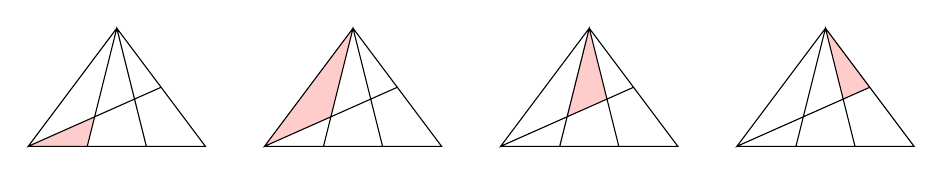
\begin{tikzpicture}[scale=.75]
      \foreach \dx/\dy/\VA/\VB/\VC in {%
        0/0/A/B/G,
        4/0/A/F/G,
        8/0/F/G/H,
        12/0/F/H/E}{%
          \begin{scope}[shift={(\dx,\dy)}]
            \coordinate(A) at (0,0);
            \coordinate(B) at (1,0);
            \coordinate(C) at (2,0);
            \coordinate(D) at (3,0);
            \coordinate(F) at (1.5,2);
            \coordinate(E) at ($.5*(D)+.5*(F)$);
            \coordinate(G) at ($.75*(B)+.25*(F)$);
            \coordinate(H) at ($.6*(C)+.4*(F)$);
            \fill[color=red!20](\VA)--(\VB)--(\VC)--cycle;
            \draw(A)--(D)--(F)--(A)--(G)--(H)--(E) (B)--(F)--(C);
          \end{scope}
        }
    \end{tikzpicture}
  \end{center}

  两个格子组成的三角形:
  \begin{center}
    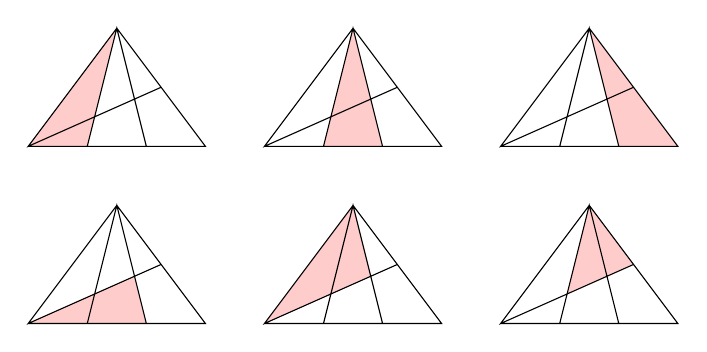
\begin{tikzpicture}[scale=.75]
      \foreach \dx/\dy/\VA/\VB/\VC in {%
        0/0/A/B/F,
        4/0/B/C/F,
        8/0/C/D/F,
        0/-3/A/C/H,
        4/-3/A/H/F,
        8/-3/G/E/F}{%
          \begin{scope}[shift={(\dx,\dy)}]
            \coordinate(A) at (0,0);
            \coordinate(B) at (1,0);
            \coordinate(C) at (2,0);
            \coordinate(D) at (3,0);
            \coordinate(F) at (1.5,2);
            \coordinate(E) at ($.5*(D)+.5*(F)$);
            \coordinate(G) at ($.75*(B)+.25*(F)$);
            \coordinate(H) at ($.6*(C)+.4*(F)$);
            \fill[color=red!20](\VA)--(\VB)--(\VC)--cycle;
            \draw(A)--(D)--(F)--(A)--(G)--(H)--(E) (B)--(F)--(C);
          \end{scope}
        }
    \end{tikzpicture}
  \end{center}

  其余3个格子、4个格子、5个格子和6个格子组成的三角形请自行考虑。
\end{proof}
\begin{proof}[另外一种数法]
  将所有的小格子排序,数出包含第一个格子所有的三角形。然后将图形挖掉第一个格子后,再数出包含第二个格子的所有的三角形。然后再继续挖掉第二个小格子,再数出包含第三个小格子的所有的三角形。依次下去可得。

  首先对小格子编号。
    \begin{center}
    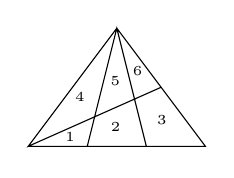
\begin{tikzpicture}[scale=.75]
      \begin{scope}[shift={(0,0)}]
        \coordinate(A) at (0,0);
        \coordinate(B) at (1,0);
        \coordinate(C) at (2,0);
        \coordinate(D) at (3,0);
        \coordinate(F) at (1.5,2);
        \coordinate(E) at ($.5*(D)+.5*(F)$);
        \coordinate(G) at ($.75*(B)+.25*(F)$);
        \coordinate(H) at ($.6*(C)+.4*(F)$);
        \draw(A)--(D)--(F)--(A)--(G)--(H)--(E) (B)--(F)--(C);
        \foreach \x/\y/\z/\v in {A/B/G/1,A/G/F/4,H/G/F/5,H/E/F/6}{%
          \node at($1/3*(\x)+1/3*(\y)+1/3*(\z)$){\tiny \v};
        }
        \foreach \x/\y/\z/\w/\v in {B/C/G/H/2,C/D/E/H/3}{%
          \node at($1/4*(\x)+1/4*(\y)+1/4*(\z)+1/4*(\w)$){\tiny \v};
        }
      \end{scope}
    \end{tikzpicture}
  \end{center}
  数出含格子1的三角形。
  \begin{center}
    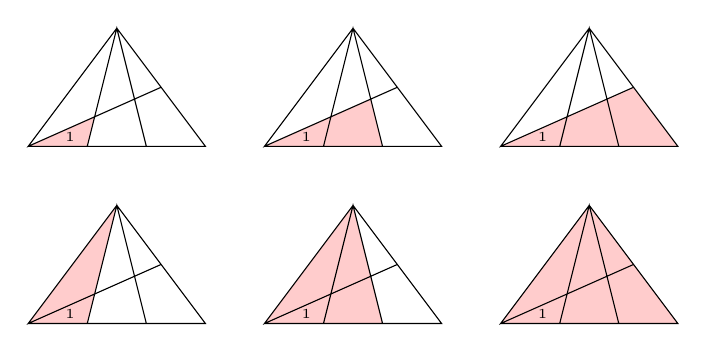
\begin{tikzpicture}[scale=.75]
      \foreach \dx/\dy/\VA/\VB/\VC in {%
        0/0/A/B/G,
        4/0/A/C/H,
        8/0/A/D/E,
        0/-3/A/B/F,
        4/-3/A/C/F,
        8/-3/A/D/F}{%
          \begin{scope}[shift={(\dx,\dy)}]
            \coordinate(A) at (0,0);
            \coordinate(B) at (1,0);
            \coordinate(C) at (2,0);
            \coordinate(D) at (3,0);
            \coordinate(F) at (1.5,2);
            \coordinate(E) at ($.5*(D)+.5*(F)$);
            \coordinate(G) at ($.75*(B)+.25*(F)$);
            \coordinate(H) at ($.6*(C)+.4*(F)$);
            \fill[color=red!20](\VA)--(\VB)--(\VC)--cycle;
            \draw(A)--(D)--(F)--(A)--(G)--(H)--(E) (B)--(F)--(C);
            \node at($1/3*(A)+1/3*(B)+1/3*(G)$){\tiny 1};
          \end{scope}
        }
    \end{tikzpicture}
  \end{center}
  挖掉格子1,找出所有包含格子2的三角形,有2个。
    \begin{center}
    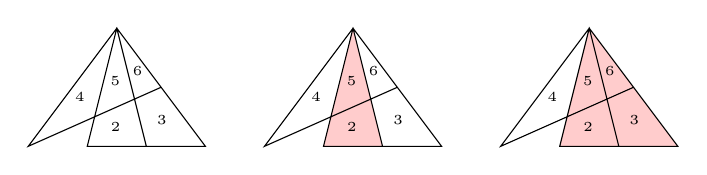
\begin{tikzpicture}[scale=.75]
      \foreach \dx/\dy/\VA/\VB/\VC in {%
        0/0/B/B/B,
        4/0/B/C/F,
        8/0/B/D/F}{%
          \begin{scope}[shift={(\dx,\dy)}]
            \coordinate(A) at (0,0);
            \coordinate(B) at (1,0);
            \coordinate(C) at (2,0);
            \coordinate(D) at (3,0);
            \coordinate(F) at (1.5,2);
            \coordinate(E) at ($.5*(D)+.5*(F)$);
            \coordinate(G) at ($.75*(B)+.25*(F)$);
            \coordinate(H) at ($.6*(C)+.4*(F)$);
            \fill[color=red!20](\VA)--(\VB)--(\VC)--cycle;
            \draw(B)--(D)--(F)--cycle (E)--(A)--(F)--(C);
            \foreach \x/\y/\z/\v in {A/G/F/4,H/G/F/5,H/E/F/6}{%
              \node at($1/3*(\x)+1/3*(\y)+1/3*(\z)$){\tiny \v};
            }
            \foreach \x/\y/\z/\w/\v in {B/C/G/H/2,C/D/E/H/3}{%
              \node at($1/4*(\x)+1/4*(\y)+1/4*(\z)+1/4*(\w)$){\tiny \v};
            }
          \end{scope}
        }
    \end{tikzpicture}
  \end{center}
  继续挖掉格子2,找出所有包含格子3的三角形,也只有1个。
    \begin{center}
    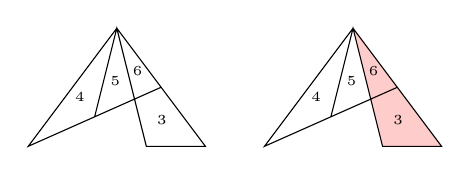
\begin{tikzpicture}[scale=.75]
      \foreach \dx/\dy/\VA/\VB/\VC in {%
        0/0/C/C/C,
        4/0/D/C/F}{%
          \begin{scope}[shift={(\dx,\dy)}]
            \coordinate(A) at (0,0);
            \coordinate(B) at (1,0);
            \coordinate(C) at (2,0);
            \coordinate(D) at (3,0);
            \coordinate(F) at (1.5,2);
            \coordinate(E) at ($.5*(D)+.5*(F)$);
            \coordinate(G) at ($.75*(B)+.25*(F)$);
            \coordinate(H) at ($.6*(C)+.4*(F)$);
            \fill[color=red!20](\VA)--(\VB)--(\VC)--cycle;
            \draw(E)--(A)--(F)--(D)--(C)--(F)--(G);
            \foreach \x/\y/\z/\v in {A/G/F/4,H/G/F/5,H/E/F/6}{%
              \node at($1/3*(\x)+1/3*(\y)+1/3*(\z)$){\tiny \v};
            }
            \foreach \x/\y/\z/\w/\v in {C/D/E/H/3}{%
              \node at($1/4*(\x)+1/4*(\y)+1/4*(\z)+1/4*(\w)$){\tiny \v};
            }
          \end{scope}
        }
    \end{tikzpicture}
  \end{center}
  继续挖掉格子3,找出所有包含格子4的三角形。
    \begin{center}
    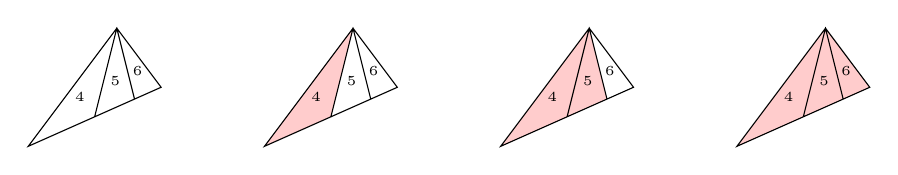
\begin{tikzpicture}[scale=.75]
      \foreach \dx/\dy/\VA/\VB/\VC in {%
        0/0/A/A/A,
        4/0/A/G/F,
        8/0/A/H/F,
        12/0/A/E/F}{%
          \begin{scope}[shift={(\dx,\dy)}]
            \coordinate(A) at (0,0);
            \coordinate(B) at (1,0);
            \coordinate(C) at (2,0);
            \coordinate(D) at (3,0);
            \coordinate(F) at (1.5,2);
            \coordinate(E) at ($.5*(D)+.5*(F)$);
            \coordinate(G) at ($.75*(B)+.25*(F)$);
            \coordinate(H) at ($.6*(C)+.4*(F)$);
            \fill[color=red!20](\VA)--(\VB)--(\VC)--cycle;
            \draw(G)--(F)--(E)--(A)--(F)--(H);
            \foreach \x/\y/\z/\v in {A/G/F/4,H/G/F/5,H/E/F/6}{%
              \node at($1/3*(\x)+1/3*(\y)+1/3*(\z)$){\tiny \v};
            }
          \end{scope}
        }
    \end{tikzpicture}
  \end{center}
  继续挖掉格子4,找出所有包含格子5的三角形,有2个。
    \begin{center}
    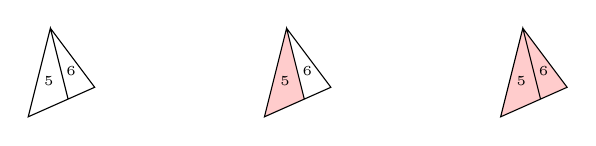
\begin{tikzpicture}[scale=.75]
      \foreach \dx/\dy/\VA/\VB/\VC in {%
        0/0/F/F/F,
        4/0/H/G/F,
        8/0/E/G/F}{%
          \begin{scope}[shift={(\dx,\dy)}]
            \coordinate(A) at (0,0);
            \coordinate(B) at (1,0);
            \coordinate(C) at (2,0);
            \coordinate(D) at (3,0);
            \coordinate(F) at (1.5,2);
            \coordinate(E) at ($.5*(D)+.5*(F)$);
            \coordinate(G) at ($.75*(B)+.25*(F)$);
            \coordinate(H) at ($.6*(C)+.4*(F)$);
            \fill[color=red!20](\VA)--(\VB)--(\VC)--cycle;
            \draw(H)--(F)--(G)--(E)--(F);
            \foreach \x/\y/\z/\v in {H/G/F/5,H/E/F/6}{%
              \node at($1/3*(\x)+1/3*(\y)+1/3*(\z)$){\tiny \v};
            }
          \end{scope}
        }
    \end{tikzpicture}
  \end{center}
  继续挖掉格子5,找出所有包含格子6的三角形,只有1个,就是格子6。
    \begin{center}
    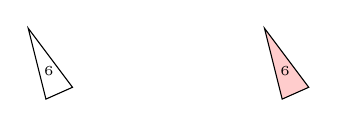
\begin{tikzpicture}[scale=.75]
      \foreach \dx/\dy/\VA/\VB/\VC in {%
        0/0/F/F/F,
        4/0/H/E/F}{%
          \begin{scope}[shift={(\dx,\dy)}]
            \coordinate(A) at (0,0);
            \coordinate(B) at (1,0);
            \coordinate(C) at (2,0);
            \coordinate(D) at (3,0);
            \coordinate(F) at (1.5,2);
            \coordinate(E) at ($.5*(D)+.5*(F)$);
            \coordinate(G) at ($.75*(B)+.25*(F)$);
            \coordinate(H) at ($.6*(C)+.4*(F)$);
            \fill[color=red!20](\VA)--(\VB)--(\VC)--cycle;
            \draw(E)--(F)--(H)--cycle;
            \foreach \x/\y/\z/\v in {H/E/F/6}{%
              \node at($1/3*(\x)+1/3*(\y)+1/3*(\z)$){\tiny \v};
            }
          \end{scope}
        }
    \end{tikzpicture}
  \end{center}
  所以所有的三角形总数是$6+2+1+3+2+1=15$。
\end{proof}

\begin{example}数一数,下面的图形中有多少个四边形?
  \begin{center}
    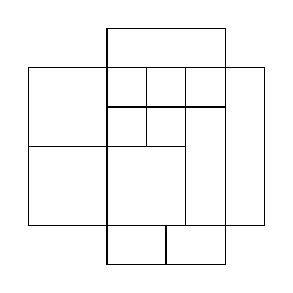
\begin{tikzpicture}[scale=.5]
      \draw(0,1)rectangle(6,5);
      \draw(2,0)rectangle(5,6);
      \draw(0,3)--(4,3)
           (3.5,0)--(3.5,1)
           (4,1)--(4,5)
           (2,4)--(5,4)
           (3,3)--(3,5);
    \end{tikzpicture}
  \end{center}
\end{example}
\begin{proof}[提示]首先最小的由单个四边形组成的共有13个。
  \begin{center}
    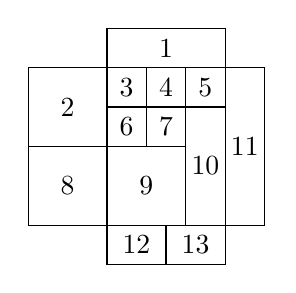
\begin{tikzpicture}[scale=.5]
      \draw(0,1)rectangle(6,5);
      \draw(2,0)rectangle(5,6);
      \draw(0,3)--(4,3)
           (3.5,0)--(3.5,1)
           (4,1)--(4,5)
           (2,4)--(5,4)
           (3,3)--(3,5);
           \foreach \n/\x/\y in{%
             1/3.5/5.5, 2/1/4, 3/2.5/4.5, 4/3.5/4.5, 5/4.5/4.5, 6/2.5/3.5, 7/3.5/3.5,
             8/1/2, 9/3/2, 10/4.5/2.5, 11/5.5/3, 12/2.75/.5, 13/4.25/.5}{%
             \node at(\x,\y){\n};
           }
    \end{tikzpicture}
  \end{center}

  由两个小四边形组成的共有9个:
  \begin{center}
    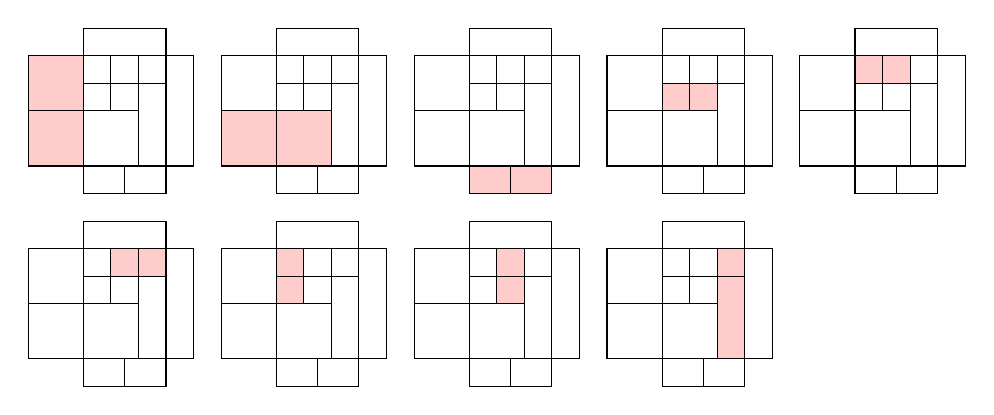
\begin{tikzpicture}[scale=.35]
      \foreach \dx/\dy/\x/\y/\xx/\yy in {%
        0/0/0/1/2/5, 7/0/0/1/4/3, 14/0/2/0/5/1, 21/0/2/3/4/4, 28/0/2/4/4/5, 
        0/7/3/4/5/5, 7/7/2/3/3/5, 14/7/3/3/4/5, 21/7/4/1/5/5
      }{
        \begin{scope}[shift={(\dx,-\dy)}]
          \fill[color=red!20](\x,\y)rectangle(\xx,\yy);
          \draw(0,1)rectangle(6,5);
          \draw(2,0)rectangle(5,6);
          \draw(0,3)--(4,3) (3.5,0)--(3.5,1) (4,1)--(4,5) (2,4)--(5,4) (3,3)--(3,5);
        \end{scope}
      }
    \end{tikzpicture}    
  \end{center}

  由三个小四边形组成的共有4个:
  \begin{center}
    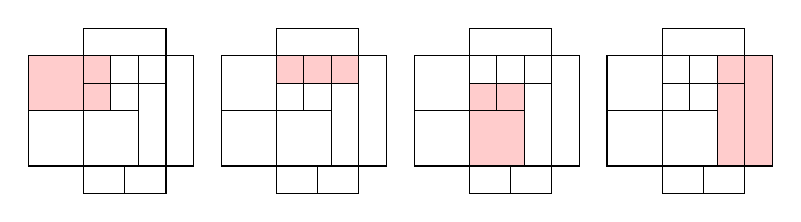
\begin{tikzpicture}[scale=.35]
      \foreach \dx/\dy/\x/\y/\xx/\yy in {%
        0/0/0/3/3/5, 7/0/2/4/5/5, 14/0/2/1/4/4, 21/0/4/1/6/5
      }{
        \begin{scope}[shift={(\dx,-\dy)}]
          \fill[color=red!20](\x,\y)rectangle(\xx,\yy);
          \draw(0,1)rectangle(6,5);
          \draw(2,0)rectangle(5,6);
          \draw(0,3)--(4,3) (3.5,0)--(3.5,1) (4,1)--(4,5) (2,4)--(5,4) (3,3)--(3,5);
        \end{scope}
      }
    \end{tikzpicture}    
  \end{center}
  
  由四个小四边形组成的共有3个:
  \begin{center}
    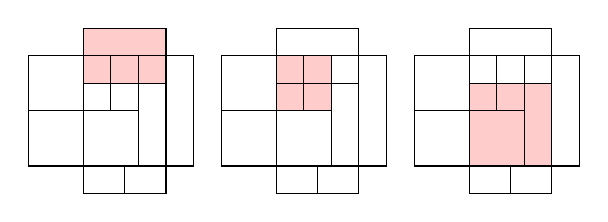
\begin{tikzpicture}[scale=.35]
      \foreach \dx/\dy/\x/\y/\xx/\yy in {%
        0/0/2/4/5/6, 7/0/2/3/4/5, 14/0/2/1/5/4
      }{
        \begin{scope}[shift={(\dx,-\dy)}]
          \fill[color=red!20](\x,\y)rectangle(\xx,\yy);
          \draw(0,1)rectangle(6,5);
          \draw(2,0)rectangle(5,6);
          \draw(0,3)--(4,3) (3.5,0)--(3.5,1) (4,1)--(4,5) (2,4)--(5,4) (3,3)--(3,5);
        \end{scope}
      }
    \end{tikzpicture}    
  \end{center}

  其余的自行考虑。
\end{proof}
\end{document}

